\subsection{Distributed approach with communication}
\label{subsec:ex1comm}

\subsubsection{Model training}
\label{subsubsec:learnedcomm}
An alternative to the previous approach involves the possibility of training a 
new distributed network that exploits a communication protocol between 
agents to decide more reliably the output control. 
Thus, using the same data collected before we build a model that at each time 
step takes as input for each robot an array containing the response values of the 
sensors – \texttt{prox\_values}, \texttt{prox\_comm} or \texttt{all\_sensors} – and 
the message received in the previous time step, communicated by the nearest 
agents (on the left and on the right), and produces as output an array of 2 floats, 
the first one is the control, which, as before, is the speed of the wheels, and the 
second one is the communication, i.e. the message transmitted by the robot to the 
nearest agents.

Also for this purpose, the model is independent of the number of agents in 
the simulations. Instead, now is important to keep track of the time steps order 
since the input of the network requires the communication received in the 
actual time step which corresponds to the messages transmitted in the previous 
one. To do so, a preprocessing is applied to the dataset to combine consecutive 
time steps into a set of sequences. Therefore, we divide each simulation in 
sequences of length $2$, composed of two successive observations for each 
robot, using a stride of $1$.   
Accordingly, the shape of the model input has been transformed from $1 \times 
\mathtt{input\_size}$ to $\mathtt{seq\_length} \times \mathtt{N} \times 
\mathtt{input\_size}$, where \texttt{seq\_length} is fixed at $2$, $N$ is variable 
and \texttt{input\_size} can be $7$ or $14$.

It is important to notice that the communication is not yet in the input since 
it is not contained in the original dataset, instead is treated as a hidden 
variable to be inferred. 
At the beginning of each sequence there are no previous time steps to 
consider since no messages have been received yet. Therefore, a placeholder 
is randomly initialised, filled with float values in the range $[0, 1]$. 
The size of this array corresponds to the number of agents plus two 
elements, one at the beginning and one at the end of the vector, always set 
to $0$, since they are used to store the fact that the two extreme robots 
never receive messages respectively from the left or from the right. 
The random initialisation of this vector is essential to increase the 
generalization capabilities of the network during its training, showing it 
different starting situations.

Another crucial aspect to consider when using communication is the type of   
updated protocol to choose. As we have already said in section 
\ref{subsec:thymiocomm}, each robot transmits a message every 0.1\gls{s} 
and likewise receives one for each of the sensors. In our case, we expect 
each agent to receive two communications, one for each of its respective 
neighbours. 
With real robots, but also in simulation, what we want to attain is a 
synchronous communication update protocol. Formally, each robot $n$, 
given the observations at time $t$, that corresponds to the sensor readings 
$S_n(t)$, and the communications at time $t-1$, in particular $C_{n-1}(t-1)$ 
and $C_{n+1}(t-1)$, calculates the control $V_n(t)$ and the message to 
transmit $C_n(t)$. 
Adopting this policy it is not important to keep track of the order of the 
robots and it is as if the agents operate simultaneously. 
Ideally, the frequency of updates must be lower than that with which the 
robots exchange messages, however it can happen that due to delays or 
noise in the sensor readings the communication of some robots is not 
received or transmitted. In this case, the array is not updated and the last 
message received is keep instead. 

As a consequence, we define a recurrent structure of the communication 
network, shown in Figure \ref{fig:commnet1}. It is composed by two nested 
modules: in the high-level operates the \texttt{CommNet} that handle the 
sensing of all the agents, while in the low-level the \texttt{SingleNet} that 
works on the sensing and the communication received by a single agent in a 
certain time step, producing as output the control and the communication to 
transmit. 
\begin{figure}[!htb]
	\centering
	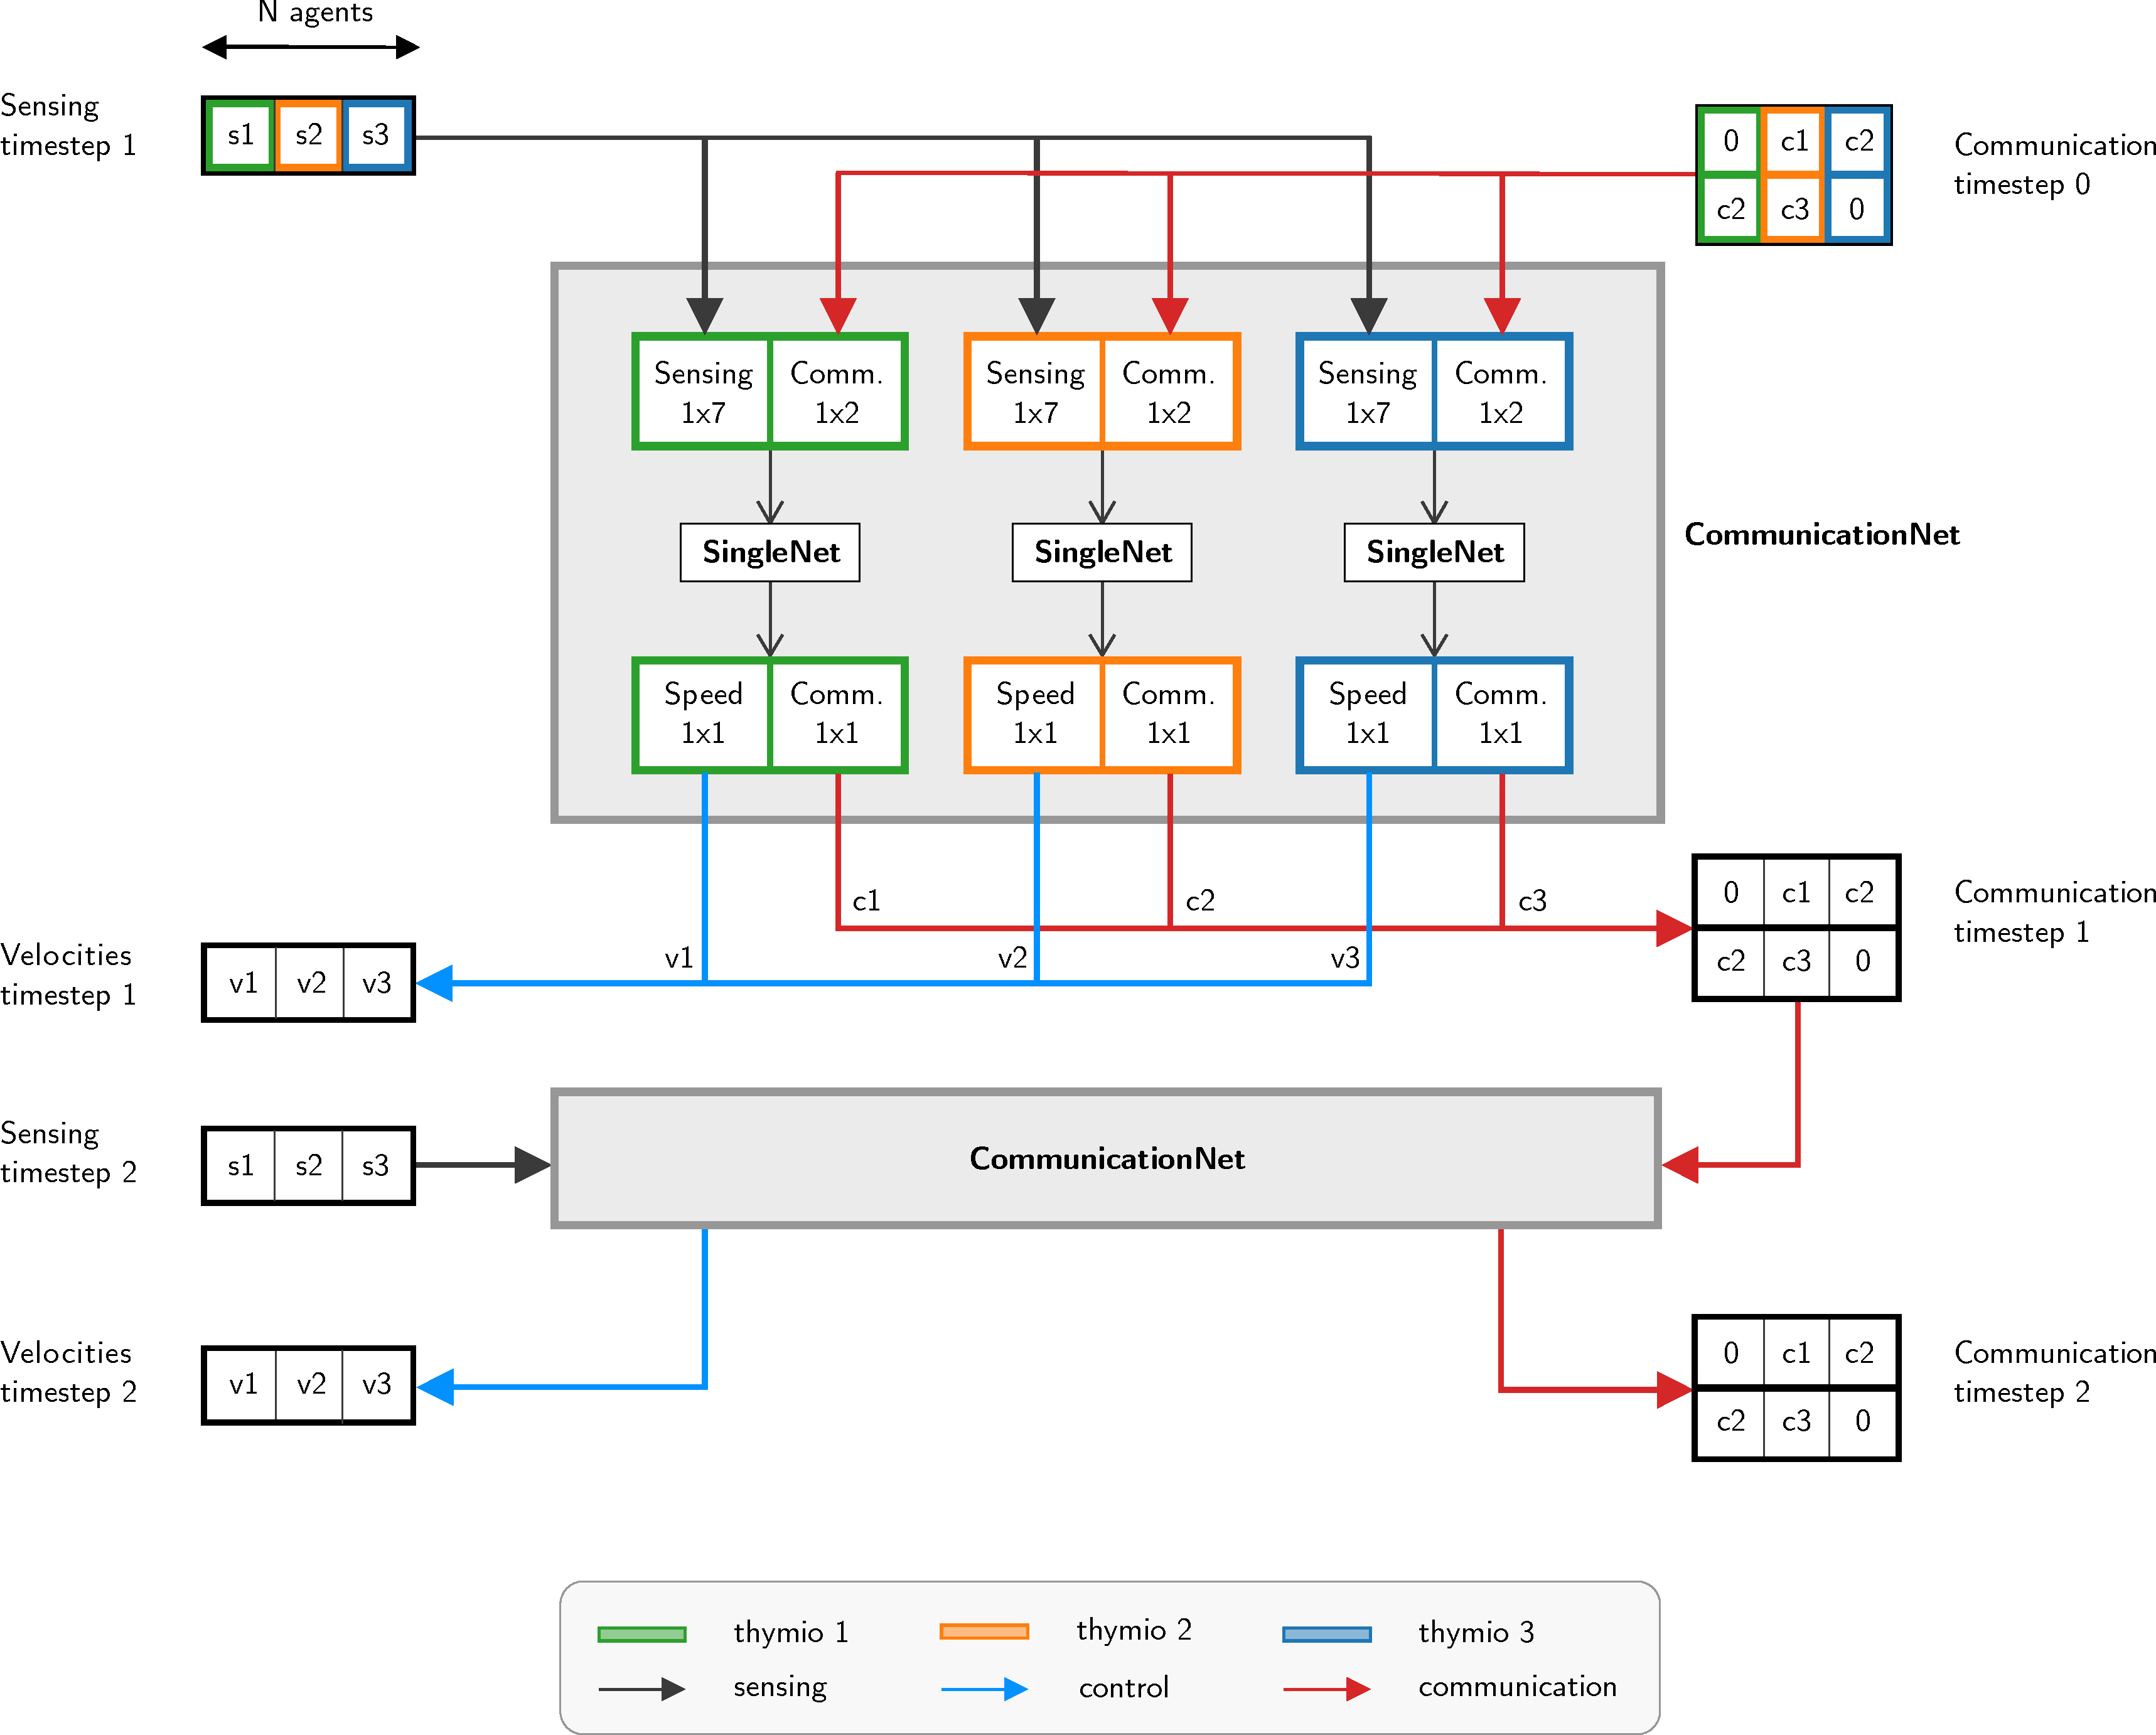
\includegraphics[width=\textwidth]{contents/images/commnet2}
	\caption[Communication network.]{Visualisation of the forward pass of the 
		communication network with three agents and a sequence composed by two 
		time steps.}
	\label{fig:commnet1}
\end{figure}

The architecture of the \texttt{SingleNet}, displayed in Figure 
\ref{fig:singlenetcomm1}, is almost the same as the one of the distributed 
model without communication: there are three linear layers each of size 
$\langle\mathtt{input\_size}, 10\rangle$,  $\langle 10, 10\rangle$ and $\langle 
10, 2\rangle$, where \texttt{input\_size} is the sum of the shape of the sensing 
and the two communication values received, one from the left and one from the 
right.

\begin{figure}[!htb]
	\centering
	\begin{subfigure}[h]{0.495\textwidth}
		\centering
		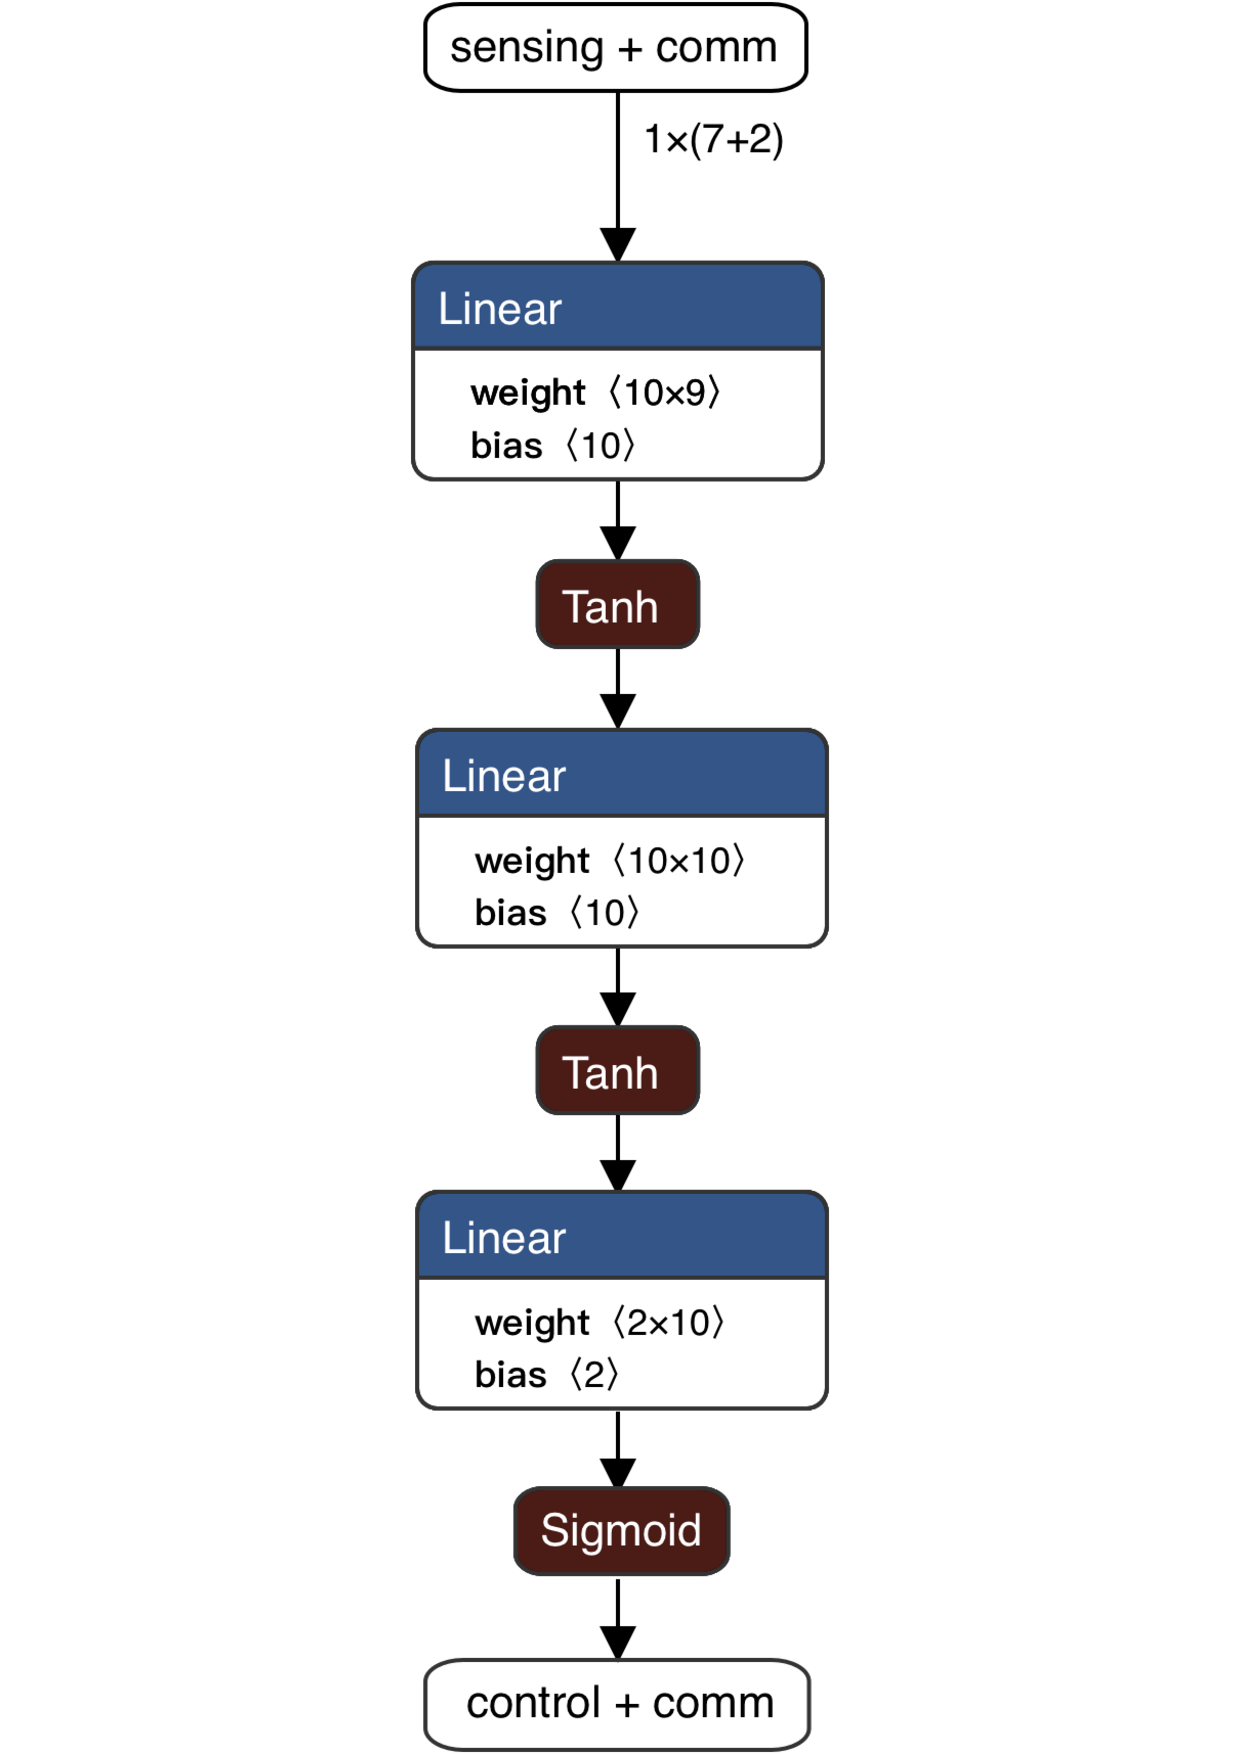
\includegraphics[width=.8\textwidth]{contents/images/task1distributedcomm@4x}%
		\caption{\texttt{SingleNet} with $7$ input sensing.}
	\end{subfigure}
	\hfill
	\begin{subfigure}[h]{0.495\textwidth}
		\centering
		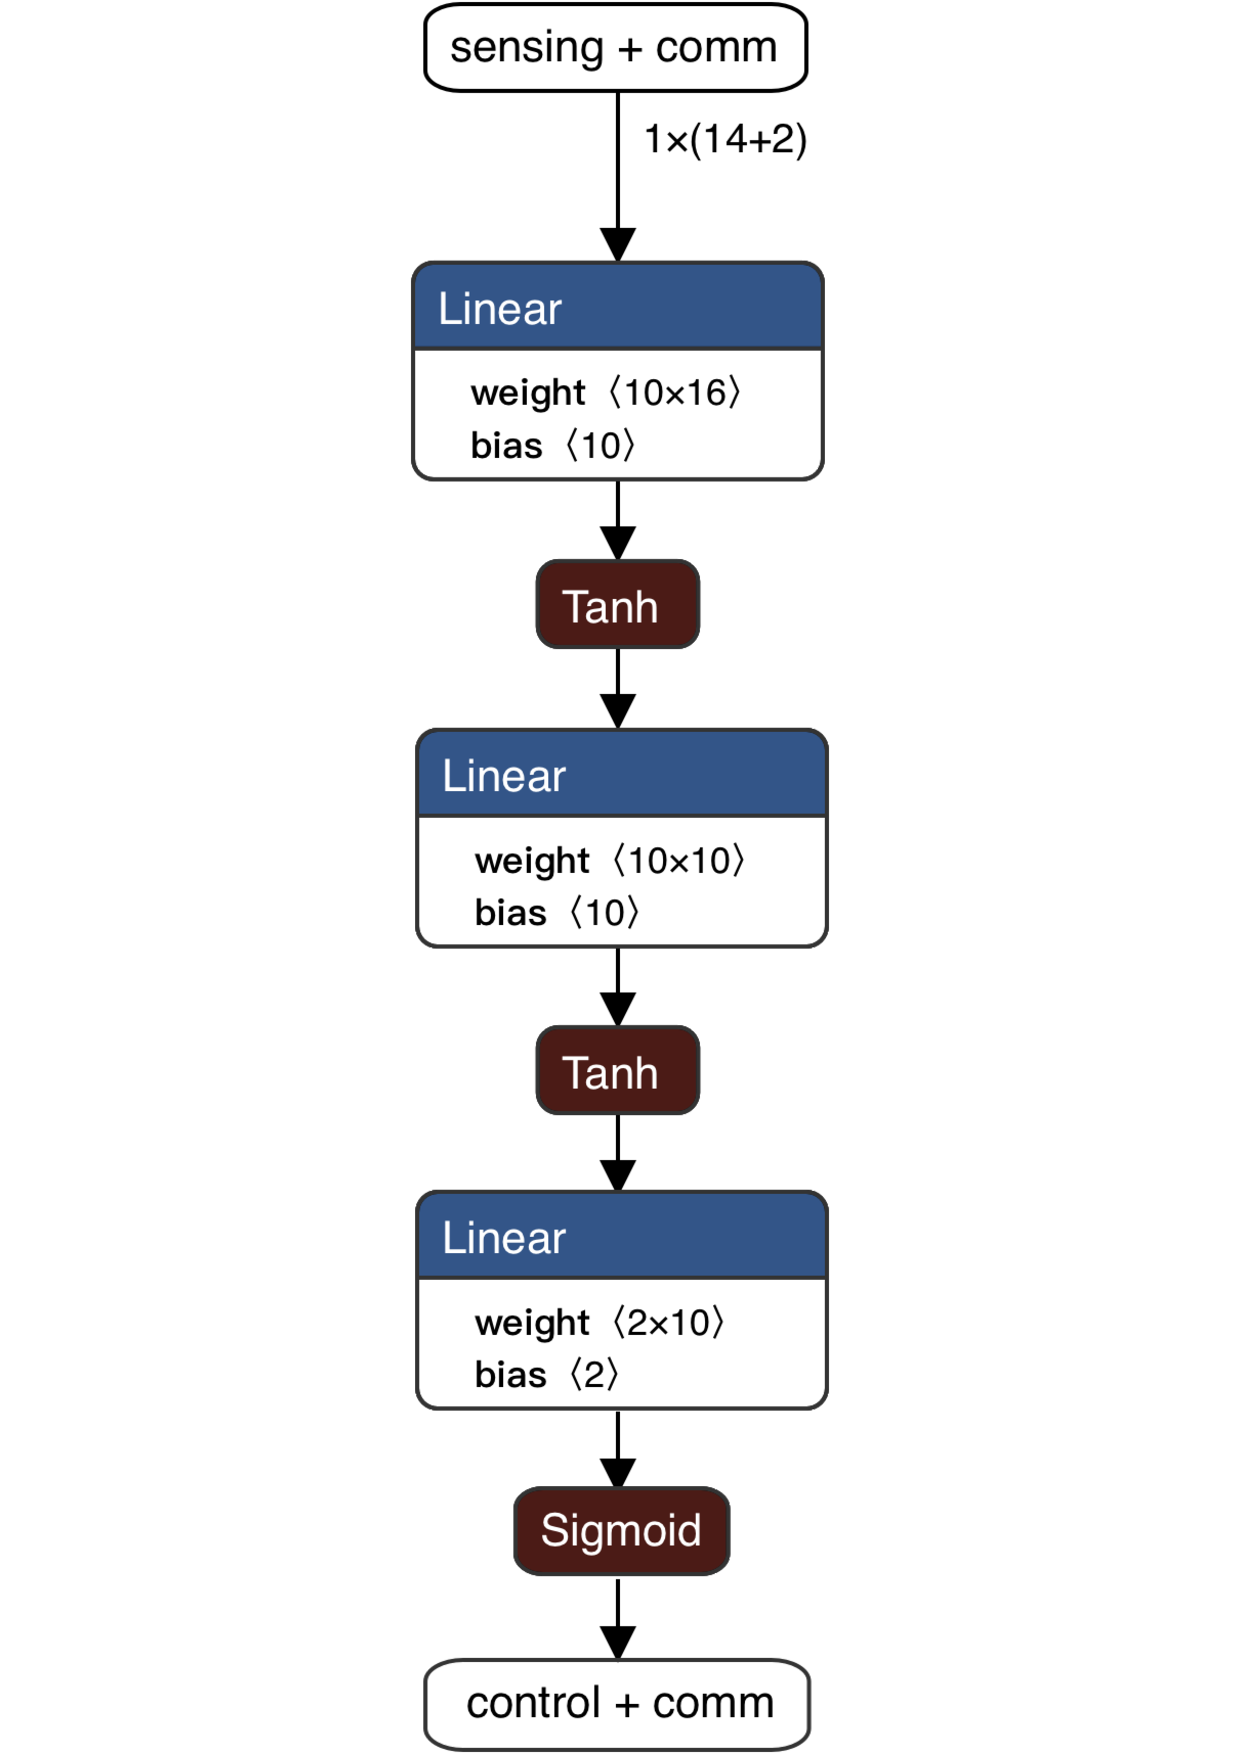
\includegraphics[width=.8\textwidth]{contents/images/task1distributed_allcomm@4x}
		\caption{\texttt{SingleNet} with $14$ input sensing.}
	\end{subfigure}
	\caption[Network architectures for the distributed approach with 
	communication.]{Visualisation of the network architecture chosen for the 
	distributed approach with communication in case of 7 or 14 inputs.}
	\label{fig:singlenetcomm1}
\end{figure}

As before, to the first and second layer is applied a Tanh non-linear 
activation function, while a sigmoid \cite[see][]{han1995influence}, shown in 
Figure \ref{fig:sigmoid}, is applied to the second dimension of the output, 
that is the value of the communication to transmit, in order to normalise it in 
the range $[0, 1]$ and its output is given by
\begin{Equation}[H]
	\centering
	\begin{equation}
	\sigma(x)= \frac{1}{1 + e - x}
	\end{equation}
	\caption{Sigmoid Function.}
	\label{eq:sigmoid}
\end{Equation}

\begin{figure}[!htb]
	\centering
	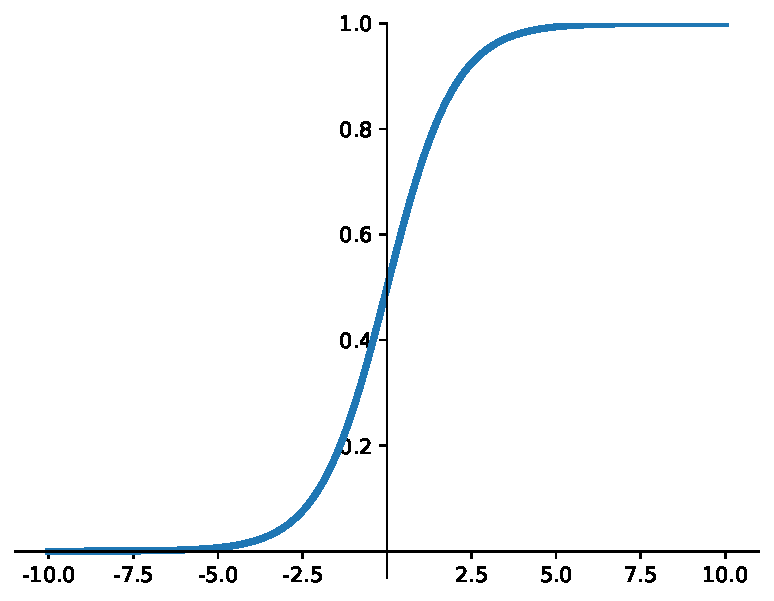
\includegraphics[width=.5\textwidth]{contents/images/sigmoid2}%
	\caption[Trend of the Sigmoid activation function.]{Trend of the Sigmoid 
	Function applied as a non-linear activation to the second output of the 
	network.}
	\label{fig:sigmoid}
\end{figure}

As before, we use Adam optimiser but with a smaller learning rate, $0.001$. 
We split the dataset in mini-batches, this time of size $10$ and then we train 
the models for $500$ epochs. 
Finally we evaluate the goodness of the predicted control using the \gls{mse} 
loss function, while the communication is learned in an unsupervised way.
Since the network is fully connected, the communication affects directly the 
output, and consequently, the error minimised, even if it is computed using 
only the control. Improving the loss has an impact also on the 
communication latent variable: since the error is propagated through the 
internal network, in order to update the weight during the back-propagation 
step, that influences the communication.

\subsubsection{Experiments}
\label{subsubsec:expcomm}

In this section we explore the same experiments carried out for the distributed 
approach without communication, paying more attention to the cases with 
variable gaps and robots. 
The first analysis, summarised in Table \ref{tab:modeln5comm}, also in this case  
concerns the behaviour of the learned controllers in case of the three different 
inputs, \texttt{prox\_values}, \texttt{prox\_comm} or 
\texttt{all\_sensors}, for a number of robots $N$ and an \texttt{avg\_gap} both 
fixed respectively at $5$ and the second chosen between $8$, $13$ and $24$.
\begin{figure}[!htb]
	\centering
	\begin{tabular}{cccc}
		\toprule
		\textbf{Model} \quad & \textbf{\texttt{network\_input}} & 
		\textbf{\texttt{input\_size}} &
		\textbf{\texttt{avg\_gap}} \\
		\midrule
		\texttt{net-c1} 				 & \texttt{prox\_values}	&  $  7$  &  $  8$  \\
		\texttt{net-c2} 			 	 & \texttt{prox\_values}	&  $  7$  &  $13$ \\
		\texttt{net-c3} 				 & \texttt{prox\_values}	&  $  7$  &  $24$  \\
		\texttt{net-c4} 				 & \texttt{prox\_comm}	  &  $  7$  &  $  8$  \\
		\texttt{net-c5} 				 & \texttt{prox\_comm}	  &  $  7$  &  $13$  \\
		\texttt{net-c6} 				 & \texttt{prox\_comm}	  &  $  7$  &  $24$  \\
		\texttt{net-c7} 				 & \texttt{all\_sensors}	  &  $14$  &  $  8$  \\
		\texttt{net-c8} 				 & \texttt{all\_sensors}	  &  $14$  &  $13$ 	\\
		\texttt{net-c9} 				 & \texttt{all\_sensors}	  &  $14$  &  $24$ 	\\
		\bottomrule
	\end{tabular}
	\captionof{table}[Experiments with $5$ agents (communication).]{List of the 
	experiments carried out with $5$ agents using communication.}
	\label{tab:modeln5comm}
\end{figure}

We start by briefly summarising in Figure \ref{fig:commlossallt} the performances 
of these model in terms of train and validation losses.
\begin{figure}[!htb]
	\centering
	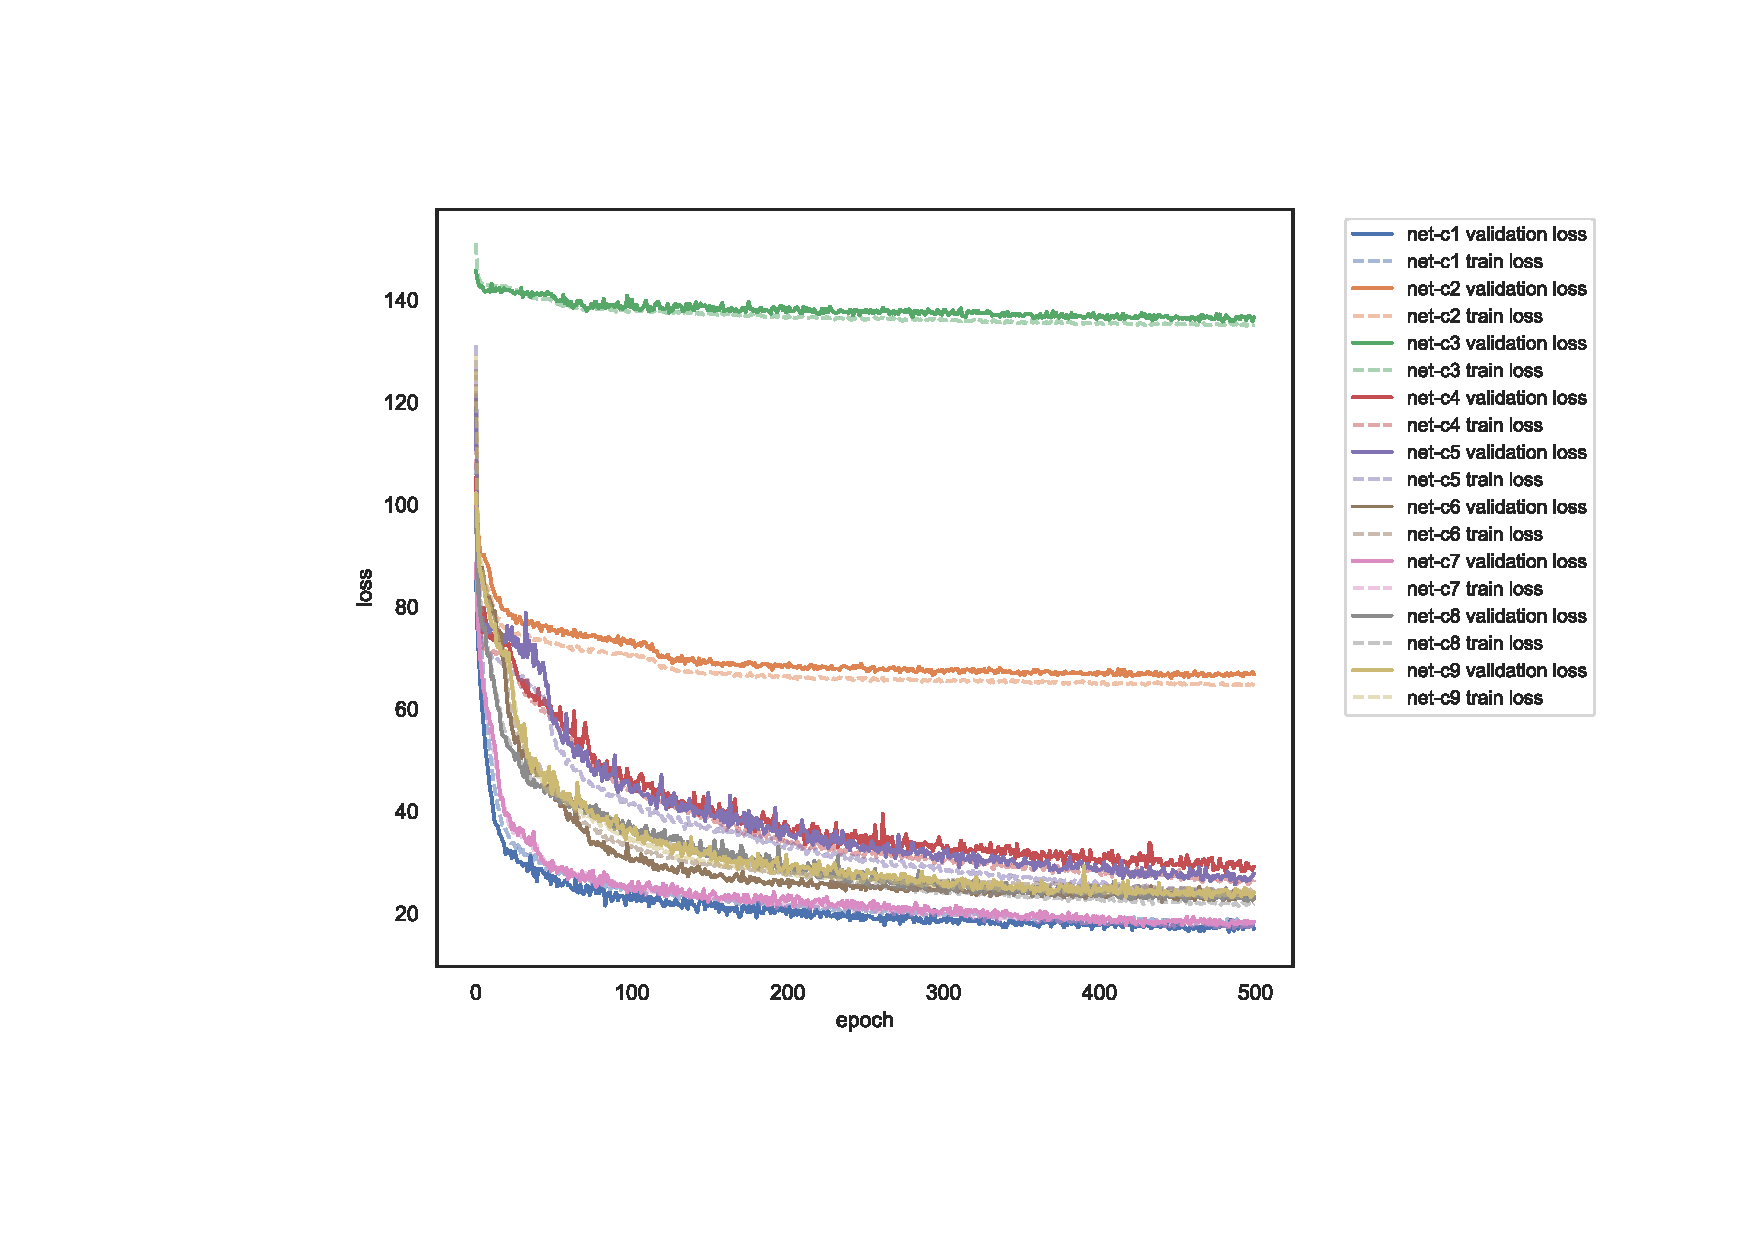
\includegraphics[width=.8\textwidth]{contents/images/task1-comm/loss-communication-all@}%
	\caption[Comparison of losses of the second set of experiments.]{Comparison 
	of the losses of the models carried out using a variable number of agents and of 
	average gap.}
	\label{fig:commlossallt}
\end{figure}
It is immediately evident that the trend of the curves are very similar to that 
obtained with the distributed approach. 

We continue by analysing and then comparing the performances obtained from 
the same experiments of the previous approach with the current one.

In Figure \ref{fig:commlossprox_values} is shown an overview of the performance, 
in terms of loss, of the models trained using \texttt{prox\_values} and varying the 
average gap: the blue, orange and green lines represent respectively gaps of $8$, 
$13$ and $24$\gls{cm}.
The loss in case of the smaller gap is decreased from $40$ to $20$, meaning an 
improvement over the previous approach.
\begin{figure}[!htb]
	\begin{center}
		\begin{subfigure}[h]{0.49\textwidth}
			\centering
			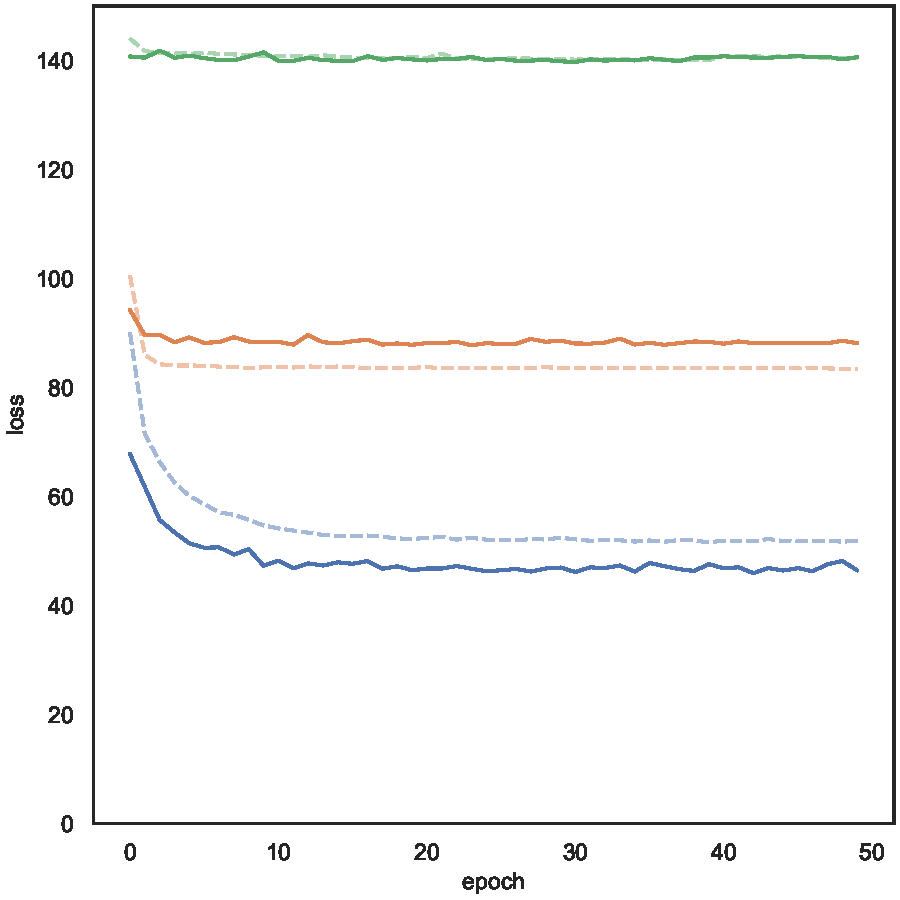
\includegraphics[width=.65\textwidth]{contents/images/task1-comm/loss-distributed-prox_values@copy}
			\caption{Distributed approach.}
		\end{subfigure}
		\hfill
		\begin{subfigure}[h]{0.49\textwidth}
			\centering
			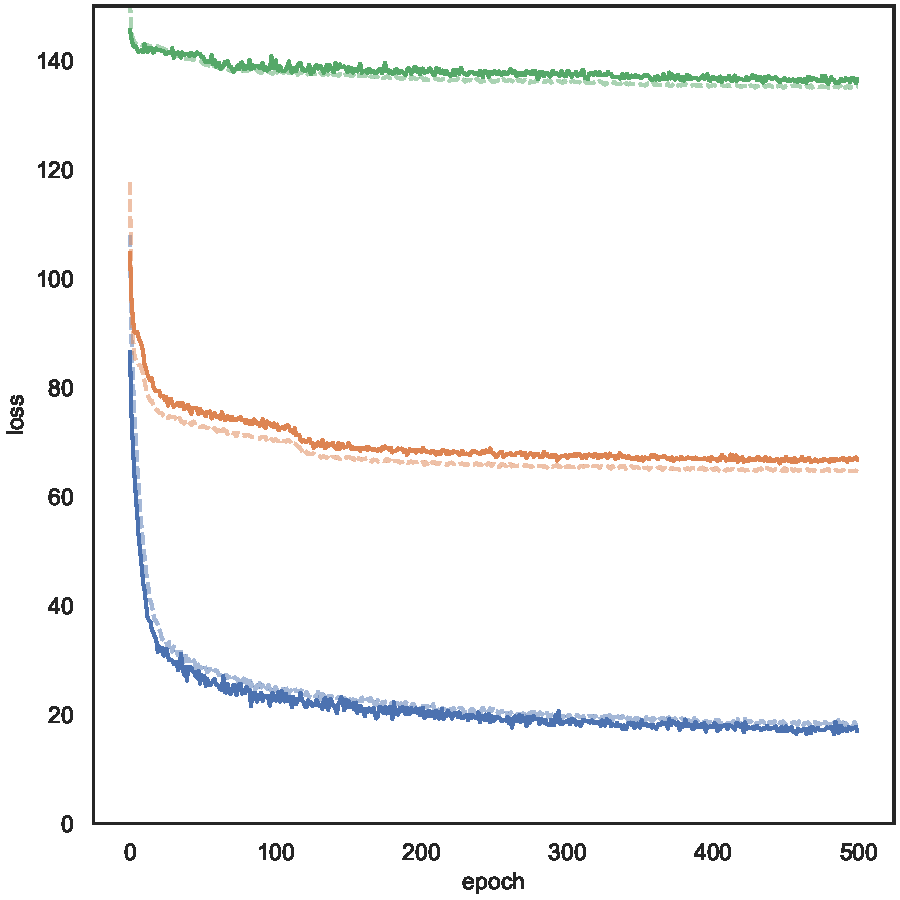
\includegraphics[width=.7\textwidth]{contents/images/task1-comm/loss-communication-prox_values@copy}
			\caption{Distributed approach with communication.}
		\end{subfigure}	
	\end{center}
\vspace{-0.5cm}
	\caption{Comparison of the losses of the models that use \texttt{prox\_values} 
		readings.}
	\label{fig:commlossprox_values}
\end{figure}

Focusing on the models that use the \texttt{prox\_values} readings as input and 
the dataset generated using $8$\gls{cm} as average gap, in Figure 
\ref{fig:net-c1r2} we observe the \gls{r2} of the manual and the learned 
controllers, in both cases, i.e. with and without communication, on the validation 
sets.
From these figures, as previously mentioned, we expect that the behaviour of the 
robots using the distributed controller instead of the manual one is better, even if 
far from the expert. On the other hand, adding the communication to the model 
produces an increase in the coefficient \gls{r2} from $0.59$ to $0.85$, thus 
promising superior performance and an attitude more similar to that of the 
omniscient controller.

\begin{figure}[!htb]
	\begin{center}
		\begin{subfigure}[h]{0.49\textwidth}
			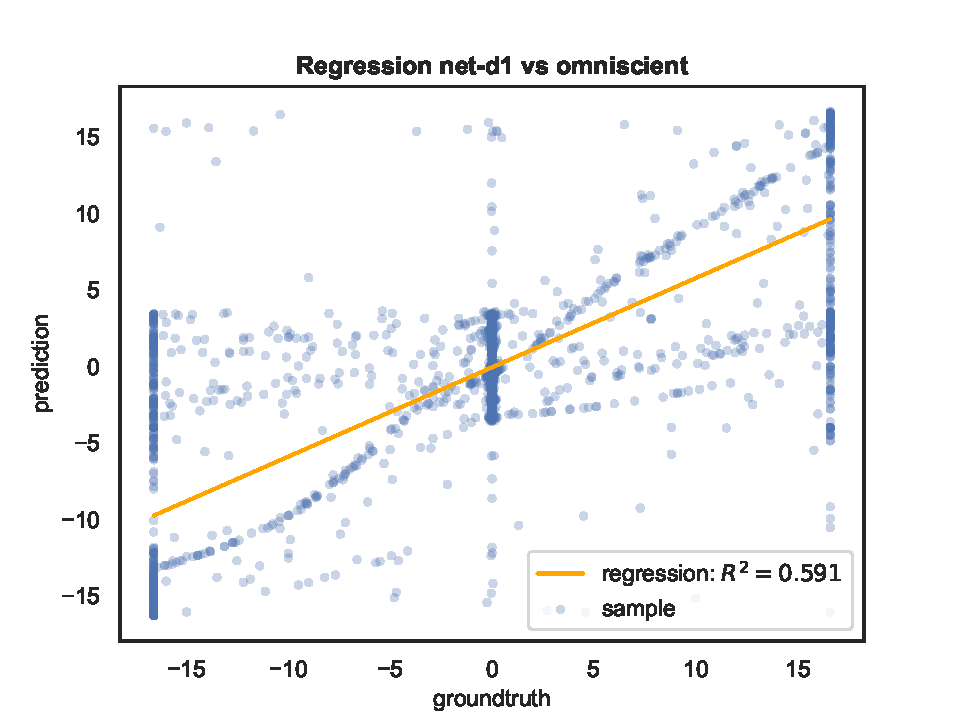
\includegraphics[width=\textwidth]{contents/images/net-d1/regression-net-d1-vs-omniscient}%
		\end{subfigure}
		\hfill\vspace{-0.5cm}
		\begin{subfigure}[h]{0.49\textwidth}
			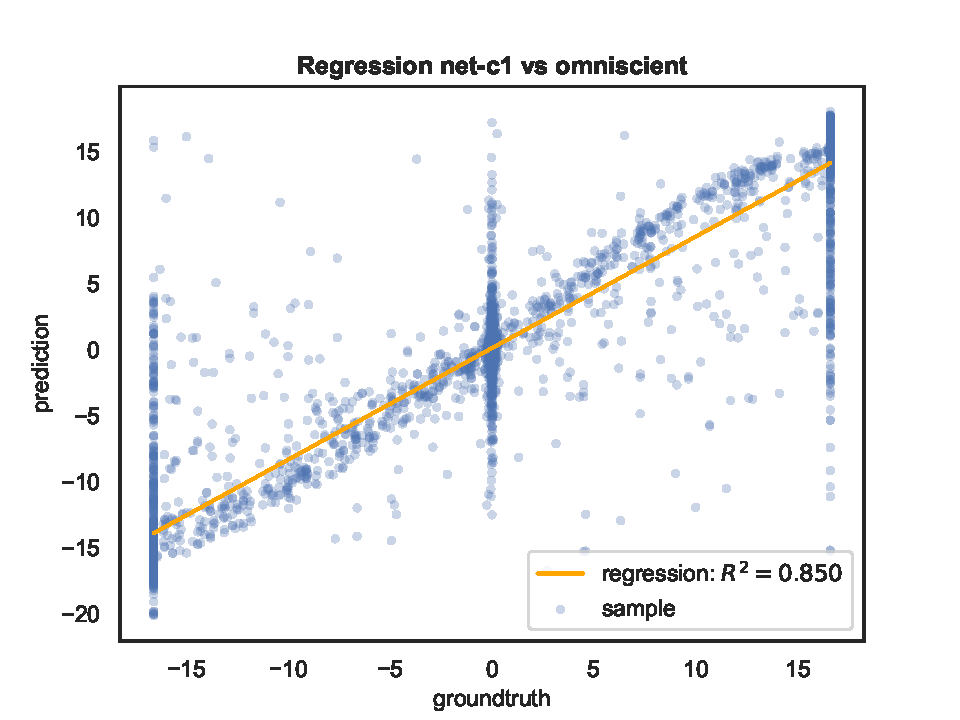
\includegraphics[width=\textwidth]{contents/images/net-c1/regression-net-c1-vs-omniscient}%
		\end{subfigure}
	\end{center}
	\caption[Evaluation of the \gls{r2} coefficients of \texttt{net-c1}.]{Comparison 
		of the \gls{r2} coefficients of the controllers learned from \texttt{net-d1} and 
		\texttt{net-c1}, with respect to the omniscient one.}
	\label{fig:net-c1r2}
\end{figure}
\begin{figure}[H]
	\begin{center}
		\begin{subfigure}[h]{0.49\textwidth}
			\centering
			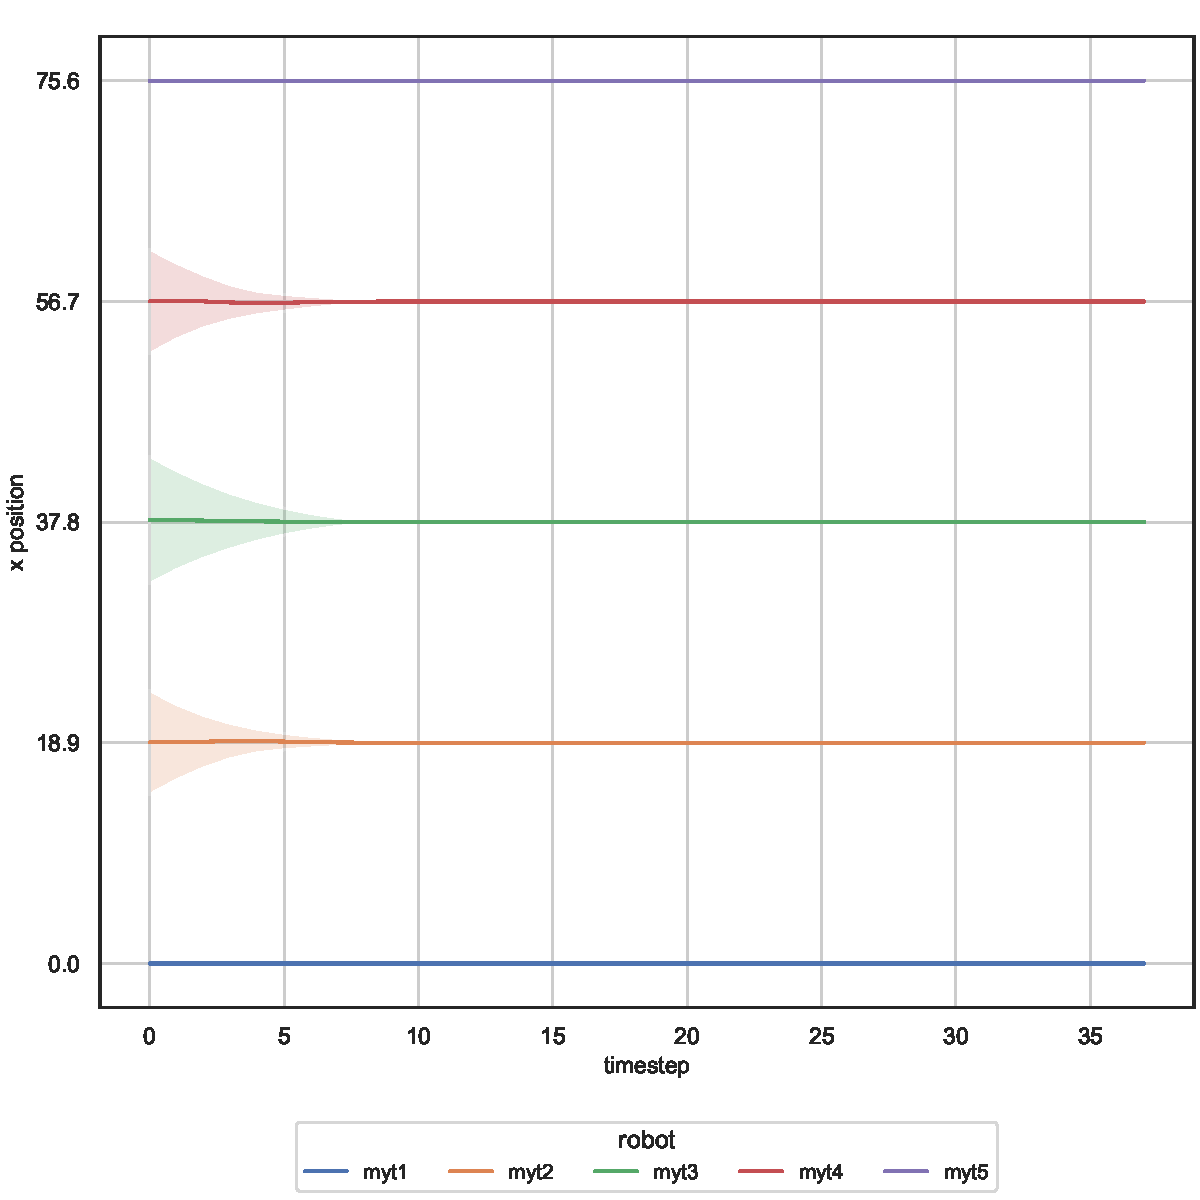
\includegraphics[width=.9\textwidth]{contents/images/net-d1/position-overtime-omniscient}%
			\caption{Expert controller trajectories.}
		\end{subfigure}
		\hfill
		\begin{subfigure}[h]{0.49\textwidth}
			\centering
			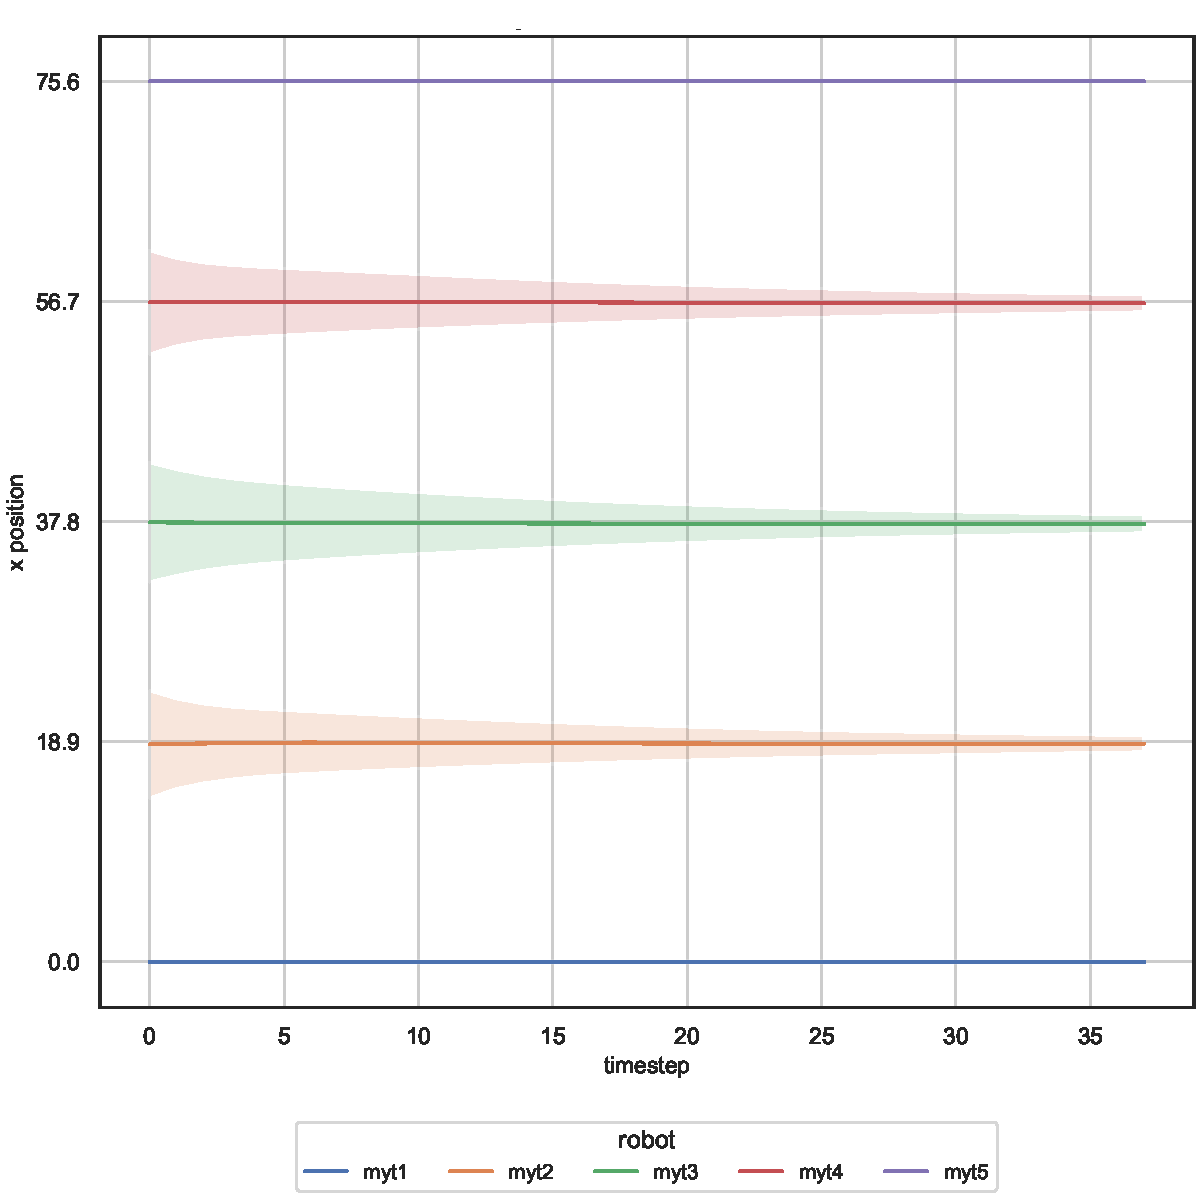
\includegraphics[width=.9\textwidth]{contents/images/net-d1/position-overtime-learned_distributed}
			\caption{Distributed controller trajectories.}
		\end{subfigure}
	\end{center}
	\begin{center}
		\begin{subfigure}[h]{0.49\textwidth}
			\centering			
			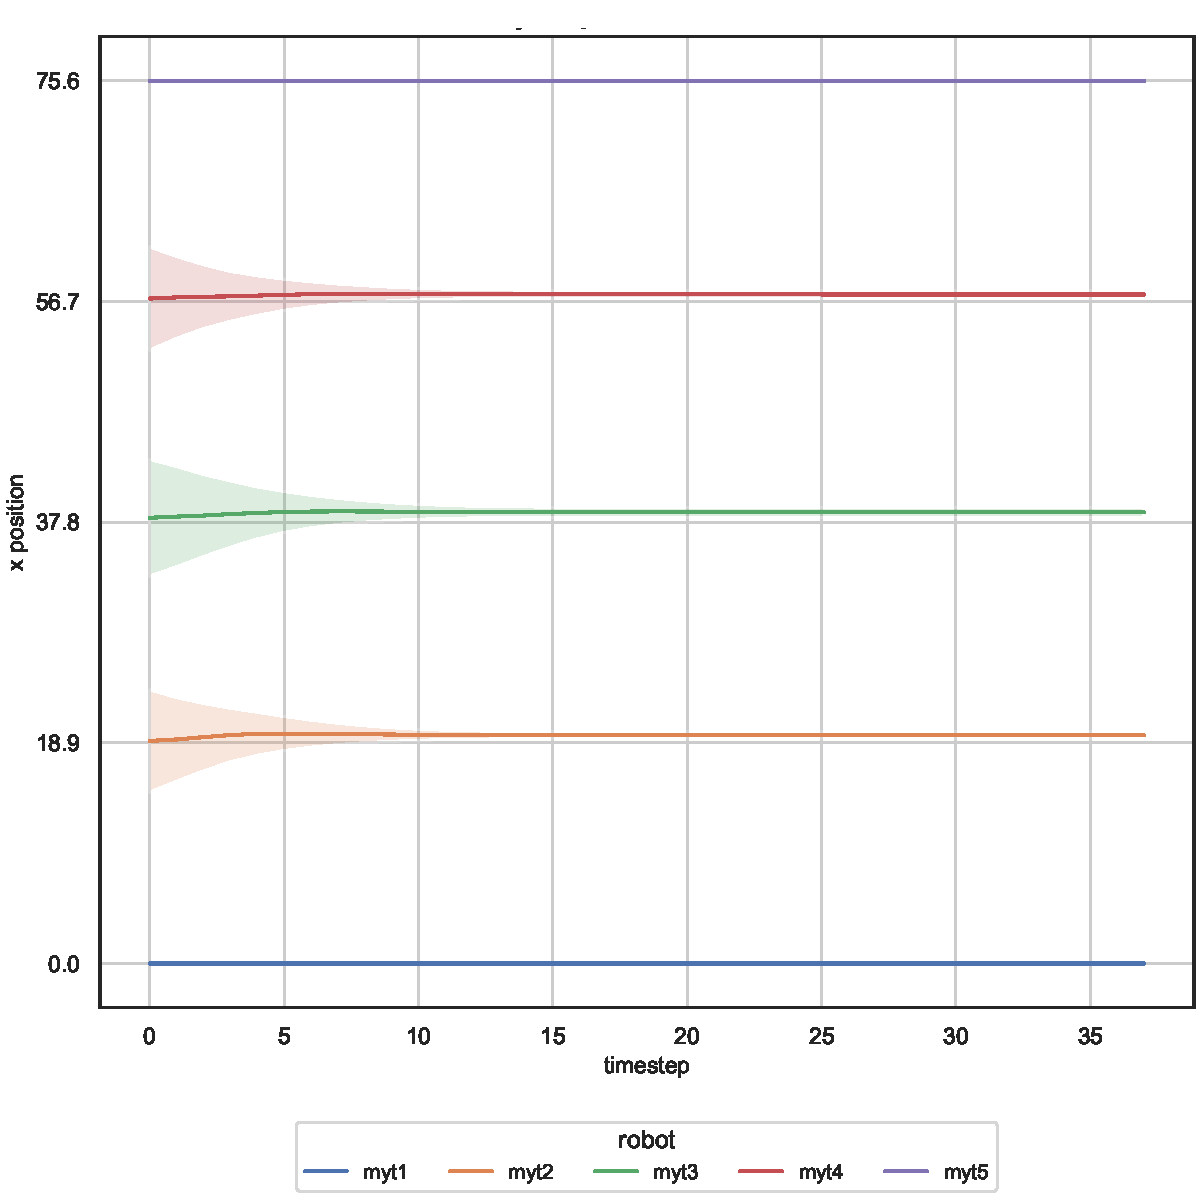
\includegraphics[width=.9\textwidth]{contents/images/net-d1/position-overtime-manual}%
			\caption{Manual controller trajectories.}
		\end{subfigure}
		\hfill
		\begin{subfigure}[h]{0.49\textwidth}
			\centering
			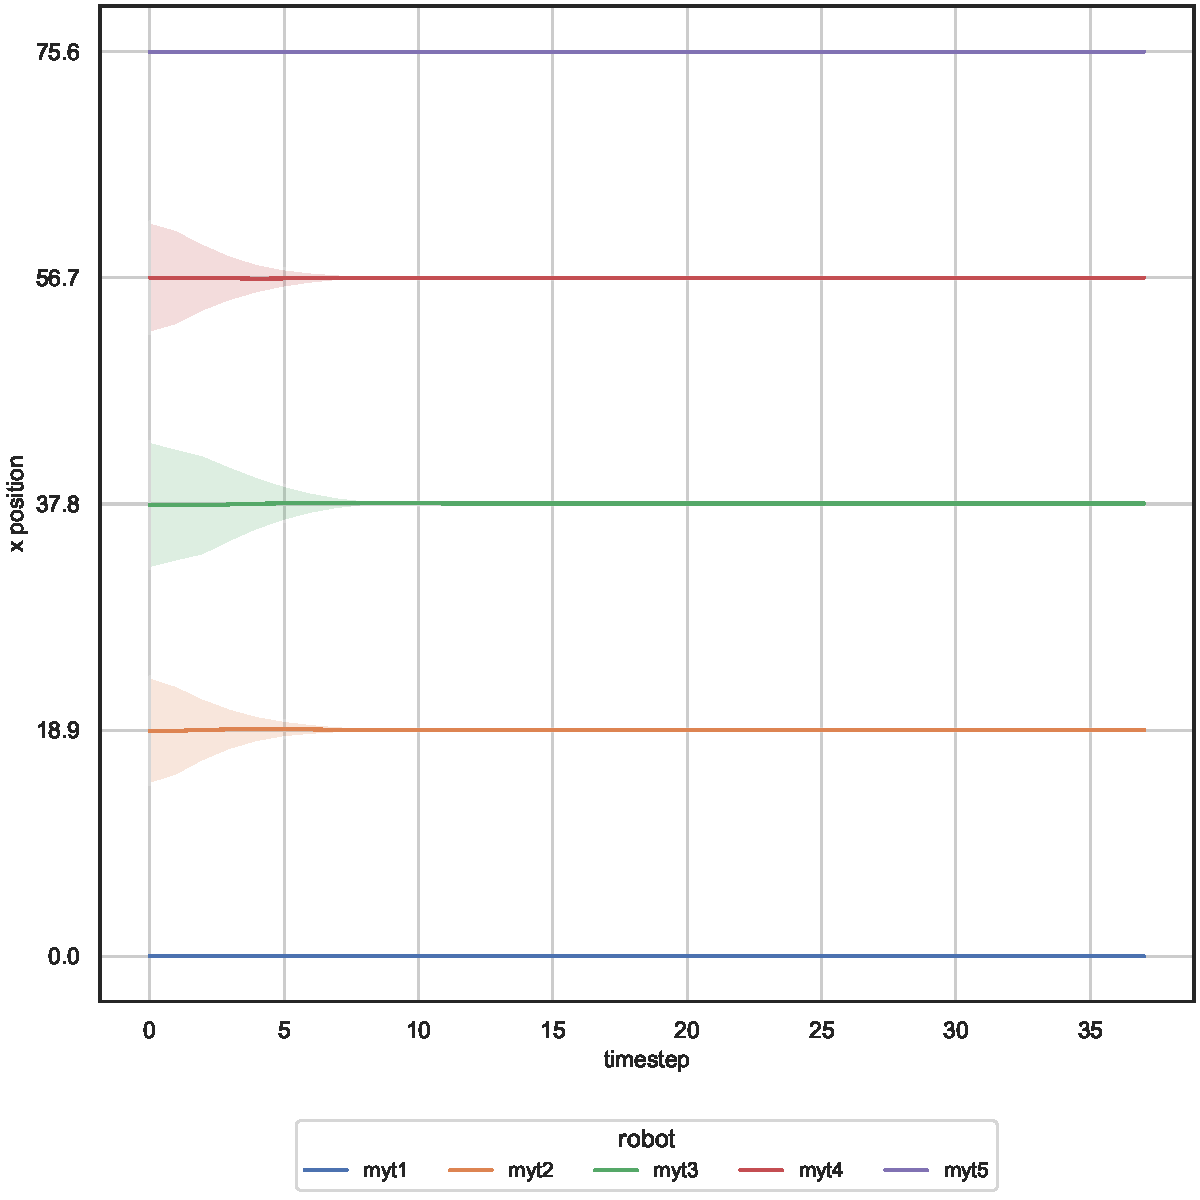
\includegraphics[width=.9\textwidth]{contents/images/net-c1/position-overtime-learned_communication}
			\caption{Communication controller trajectories.}
		\end{subfigure}
	\end{center}
	\vspace{-0.5cm}
	\caption[Evaluation of the trajectories learned by \texttt{net-c1}.]{Comparison 
	of trajectories generated using four controllers: the expert, the manual and the 
	two learned from \texttt{net-d1} and \texttt{net-c1}.}
	\label{fig:net-c1traj}
\end{figure}

To confirm this improvement, we show in Figure \ref{fig:net-c1traj} the 
trajectories obtained employing the four controllers. 
Clearly, the convergence of the robots to the target using the communication is 
much faster that with the distributed controller alone, but it is even better than 
the manual, to such an extent that it can be compared to the expert.

Moreover, analysing the evolution of the control over time in Figure 
\ref{fig:net-c1control}, we observe that this time the control learned from the 
network with communication is much more similar to that decided by the expert.
After about $10$ time steps both reach the target and set the speed at $0$, while 
the manual and the distributed need more time.

\begin{figure}[!htb]
	\begin{center}
		\begin{subfigure}[h]{0.35\textwidth}
			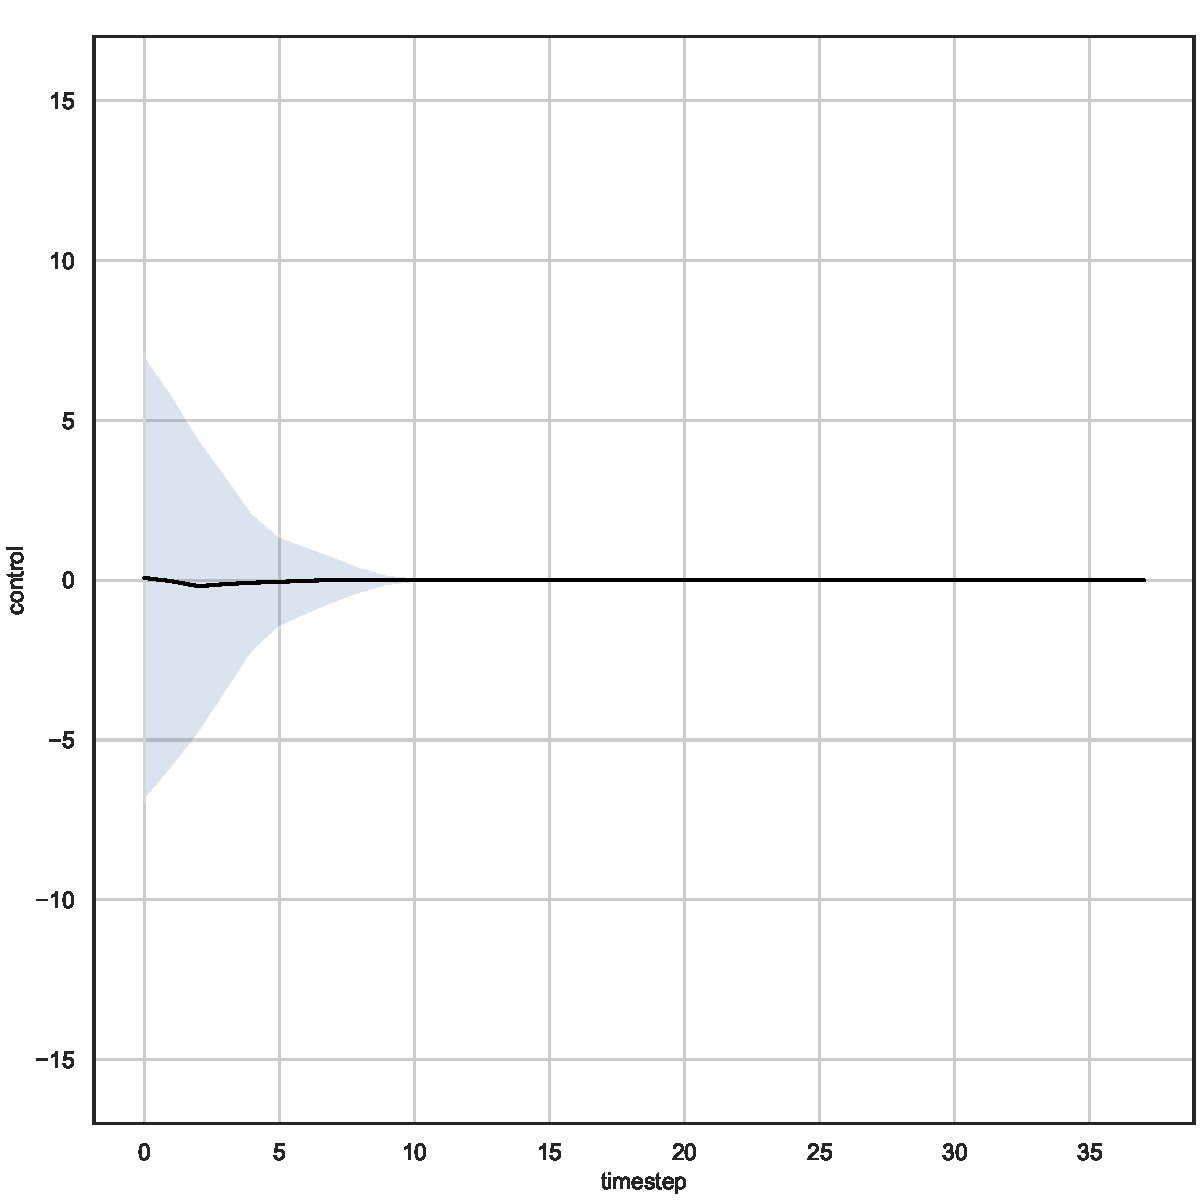
\includegraphics[width=\textwidth]{contents/images/net-d1/control-overtime-omniscient}%
			\caption{Expert control.}
		\end{subfigure}
		\hspace{1cm}
		\begin{subfigure}[h]{0.35\textwidth}
			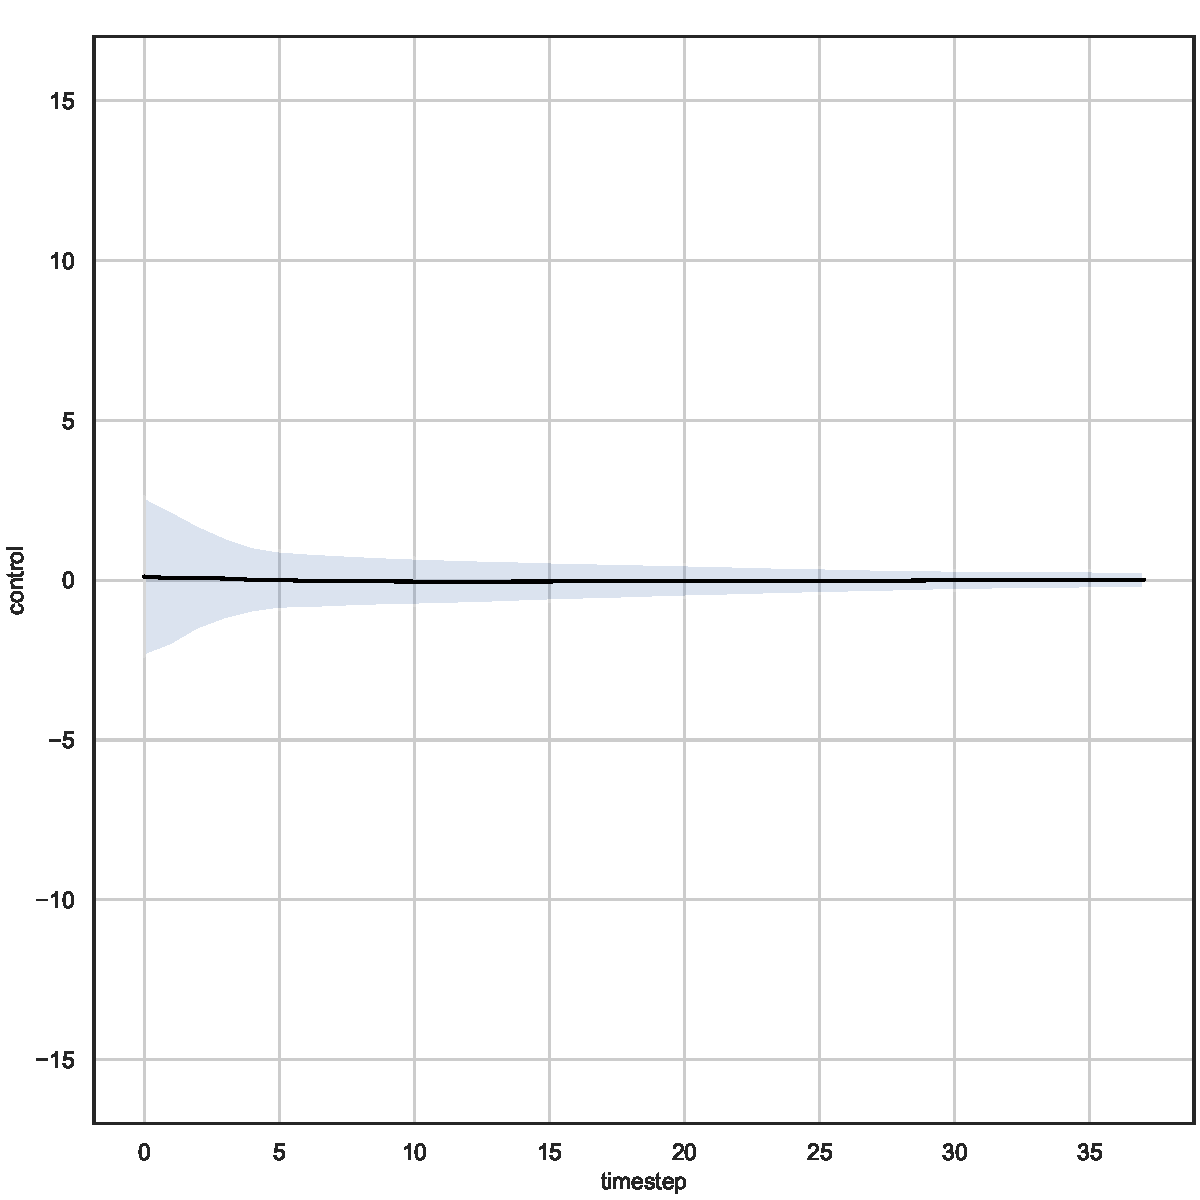
\includegraphics[width=\textwidth]{contents/images/net-d1/control-overtime-learned_distributed}
			\caption{Distributed control.}
		\end{subfigure}
	\end{center}
	\begin{center}
		\begin{subfigure}[h]{0.35\textwidth}			
			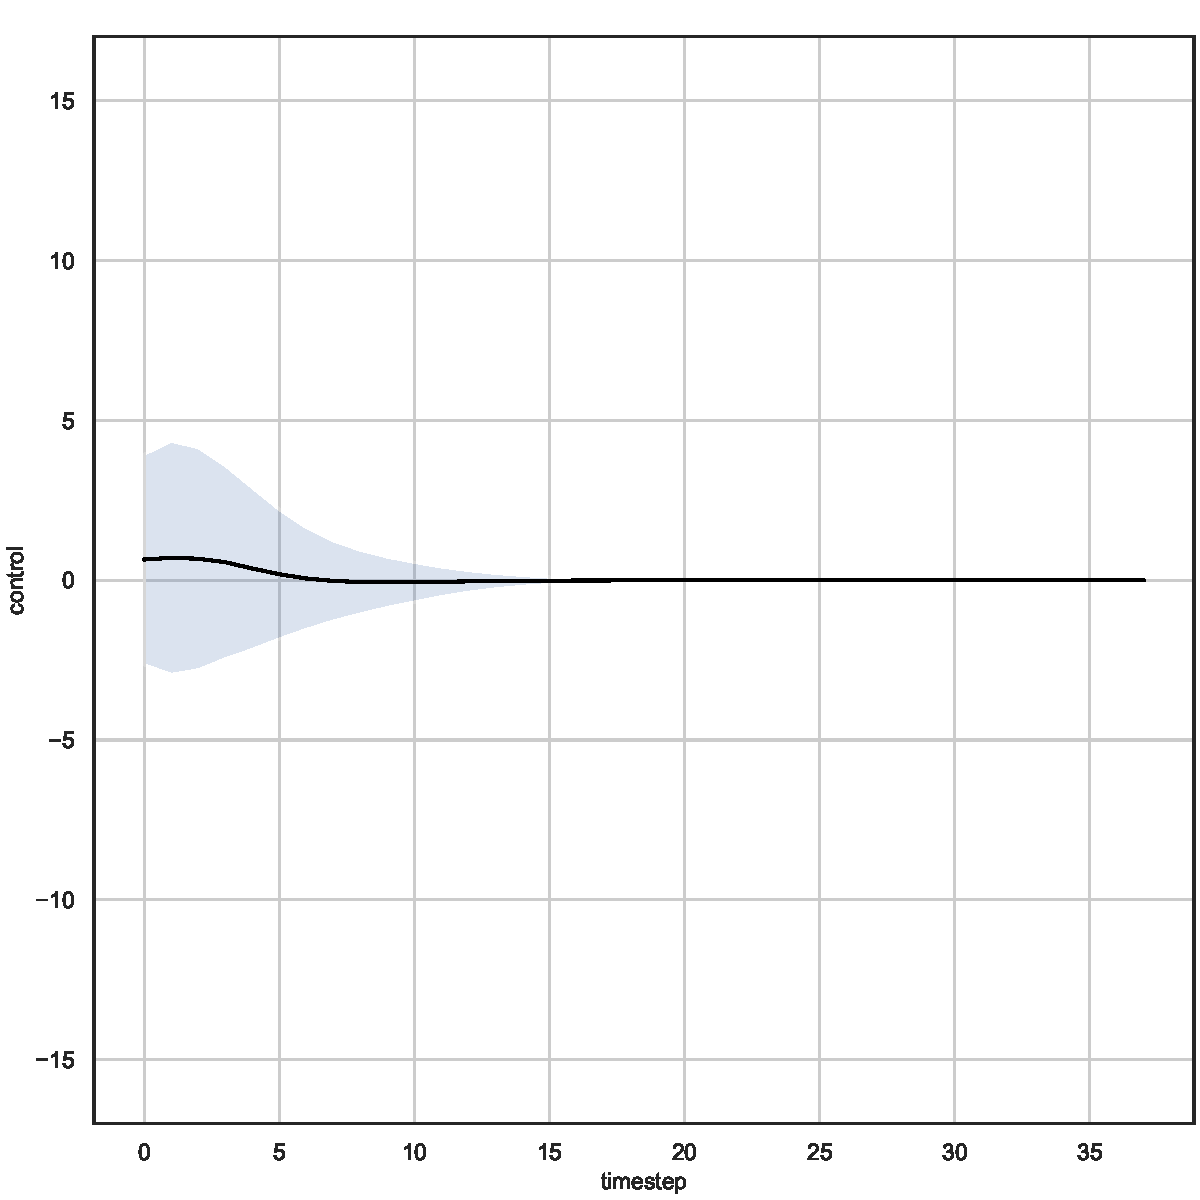
\includegraphics[width=\textwidth]{contents/images/net-d1/control-overtime-manual}%
			\caption{Manual control.}
		\end{subfigure}
		\hspace{1cm}
		\begin{subfigure}[h]{0.35\textwidth}
			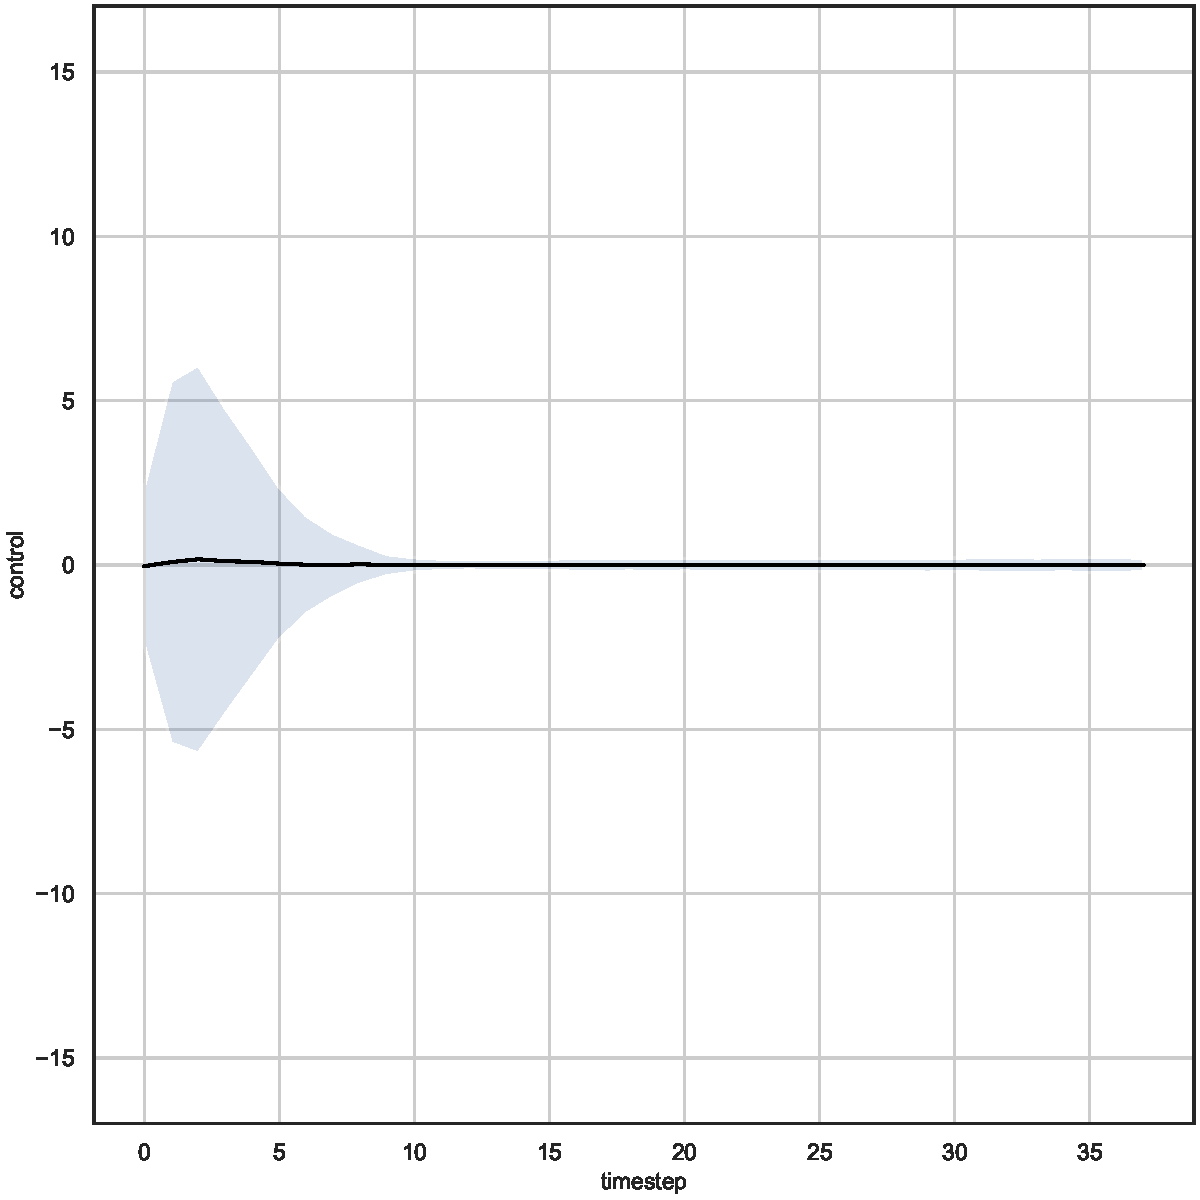
\includegraphics[width=\textwidth]{contents/images/net-c1/control-overtime-learned_communication}
			\caption{Communication control.}
		\end{subfigure}
	\end{center}
	\vspace{-0.5cm}
	\caption[Evaluation of the control decided by \texttt{net-c1}.]{Comparison of 
		output control decided using four controllers: the expert, the manual and the 
		two learned from \texttt{net-d1} and \texttt{net-c1}.}
	\label{fig:net-c1control}
\end{figure}

In Figure \ref{fig:net-c1responseposition} is displayed the behaviour of a robot 
located between two stationary agents which are already in the correct position, 
showing the response of the controllers, on the y-axis, by varying the position of 
the moving robot, on the x-axis.  
As expected, the output is a high value, positive or negative when the robot is 
near to an obstacle on the left or on the right, or close to $0$ when the distance is 
equal on both side.
When the moving robot is located halfway between the two stationary agents, the 
behaviour of the controller with communication is more similar to the one desired.
\begin{figure}[!htb]
	\centering
	\includegraphics[width=.45\textwidth]{contents/images/net-c1/response-varying_init_position-communication}%
	\caption{Response of \texttt{net-c1} by varying the initial position.}
	\label{fig:net-c1responseposition}
\end{figure}

Finally, in Figure \ref{fig:net-c1distance} are presented the absolute distances of 
each robot from the target, visualised on the y-axis, over time.
On average, the distance from goal of the communication controller is far better  
than that obtained with the distributed and the manual. After about $5$ time 
steps the robots are in the final configuration, while using the distributed 
alone, $25$ time steps are necessary to get closer to the target. Instead, the 
manual controller does not reach the goal, remaining $1$\gls{cm} away. 
\begin{figure}[!htb]
	\centering
	\includegraphics[width=.65\textwidth]{contents/images/net-c1/distances-from-goal-compressed-communication}%
	\caption[Evaluation of \texttt{net-c1} distances from goal.]{Comparison of 
		performance in terms of distances from goal obtained using four controllers: 
		the expert, the manual and the two learned from \texttt{net-d1} and 
		\texttt{net-c1}.}
	\label{fig:net-c1distance}
\end{figure}

\begin{figure}[!htb]
	\centering
	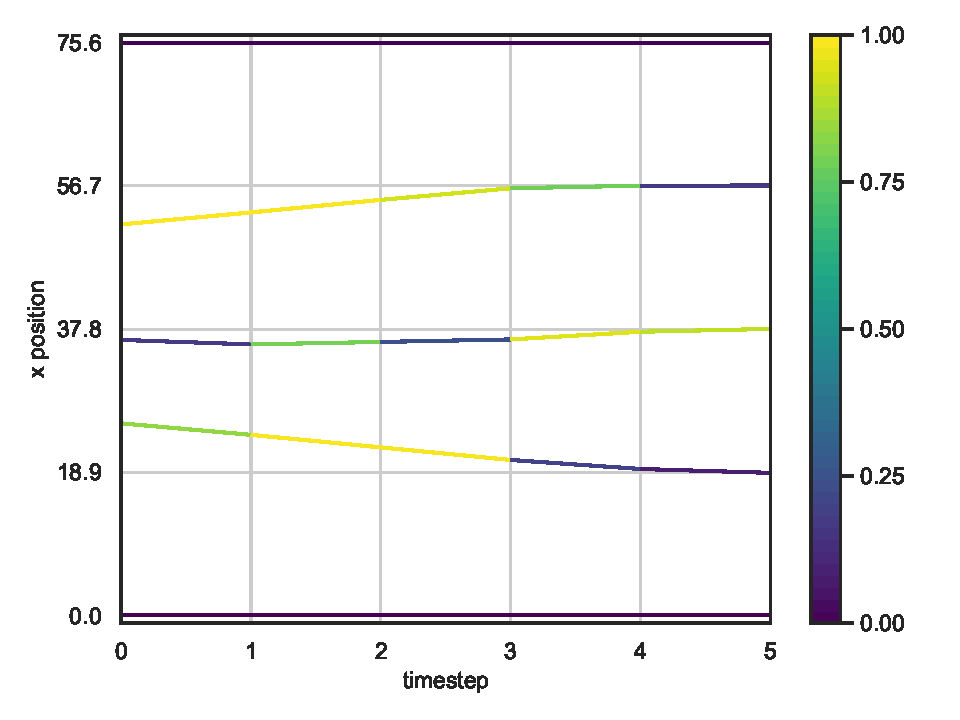
\includegraphics[width=.65\textwidth]{contents/images/net-c1/0/plot-simulation-communication-0}
	\vspace{-0.5cm}
	\caption[Evaluation of the communication learned by 
	\texttt{net-c1}.]{Visualisation of the communication values transmitted by each 
		robot over time using the controller learned from \texttt{net-c1}.}	
	\label{fig:net-c1comm}
\end{figure}
For this experiment it seems that the addition of the communication allowed the 
distributed controller to assume an efficient behaviour, for this reason it is 
interesting to investigate how this happens since the communication protocol is 
inferred and learned from the network.
Analysing the graph in Figure \ref{fig:net-c1comm}, which shows the trajectories 
of the agents over time coloured in such a way that the messages transmitted are 
shown through a colour bar whose spectrum is included in the range $[0, 1]$, i.e. 
the maximum and minimum value of communication transmitted. 
We observe that the second and fourth robots in the first time steps transmit 
values close to one, while the central one transmits a value very close to 0. 
The agents begin to move towards the desired position and, as they approach the 
target, the extreme ones transmit decreasing values while the central one 
transmits a higher value. In this case, 5 time steps are sufficient to reach the final 
configuration.
It is difficult, however, only from this image to understand the policy with which 
the network decides the communication policy.
From a further analysis in fact it would seem that the value predicted by the 
network is not linearly correlated neither to the distance from the goal nor to the 
speed assumed by the agents.

Following are presented the results of the experiments performed using 
\texttt{prox\_comm}
\begin{figure}[!htb]
	\begin{center}
		\begin{subfigure}[h]{0.49\textwidth}
			\centering
			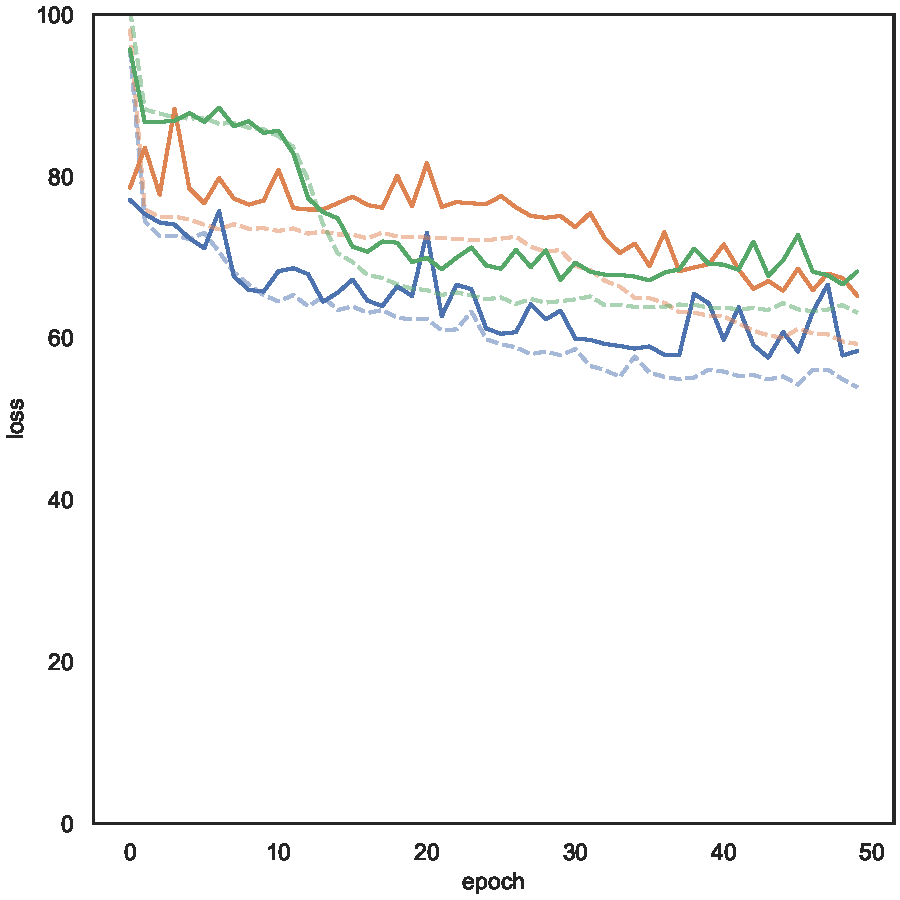
\includegraphics[width=.7\textwidth]{contents/images/task1-comm/loss-distributed-prox_comm@copy}
			\caption{Distributed approach.}
		\end{subfigure}
		\hfill
		\begin{subfigure}[h]{0.49\textwidth}
			\centering
			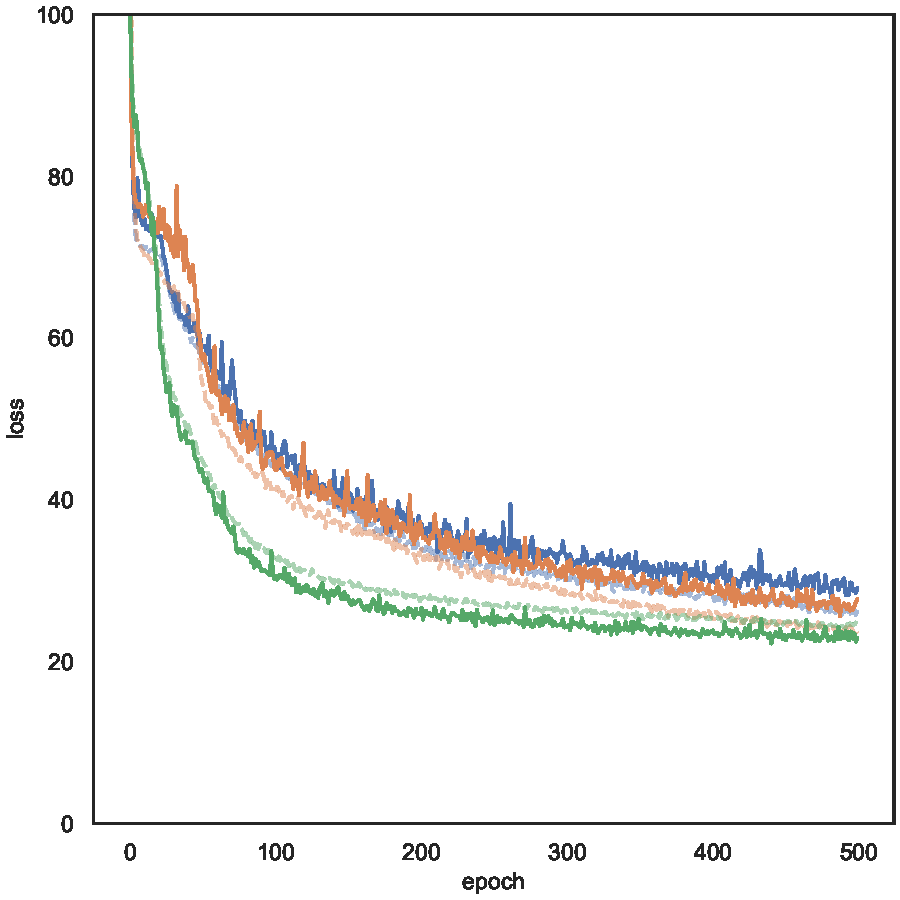
\includegraphics[width=.7\textwidth]{contents/images/task1-comm/loss-communication-prox_comm@copy}
			\caption{Distributed approach with communication.}
		\end{subfigure}	
	\end{center}
	\vspace{-0.5cm}
	\caption{Comparison of the losses of the models that use \texttt{prox\_comm} 
		readings.}
	\label{fig:commlossprox_comm}
\end{figure}

\noindent
 readings. In Figure \ref{fig:commlossprox_comm}, are 
shown the losses by varying the average gap, as before the blue, orange and 
green lines represent respectively gaps of $8$, $13$ and $24$\gls{cm}. From a 
first observation, the network seems to be able to work with all the gaps and the  
approach with communication demonstrate lower loss values than the previous 
one.

Focusing on the models that use the dataset generate using $24$\gls{cm} as 
average gap, in Figure \ref{fig:net-c6r2} we observe the \gls{r2} of the manual 
and the learned controllers, both the one with and the one without 
communication, on the validation sets.
Once again, we expect better performance using the new approach than the 
previous, given the fact that the coefficient is increased from $0.55$ up to $0.85$.
\begin{figure}[!htb]
	\begin{center}
		\begin{subfigure}[h]{0.49\textwidth}
			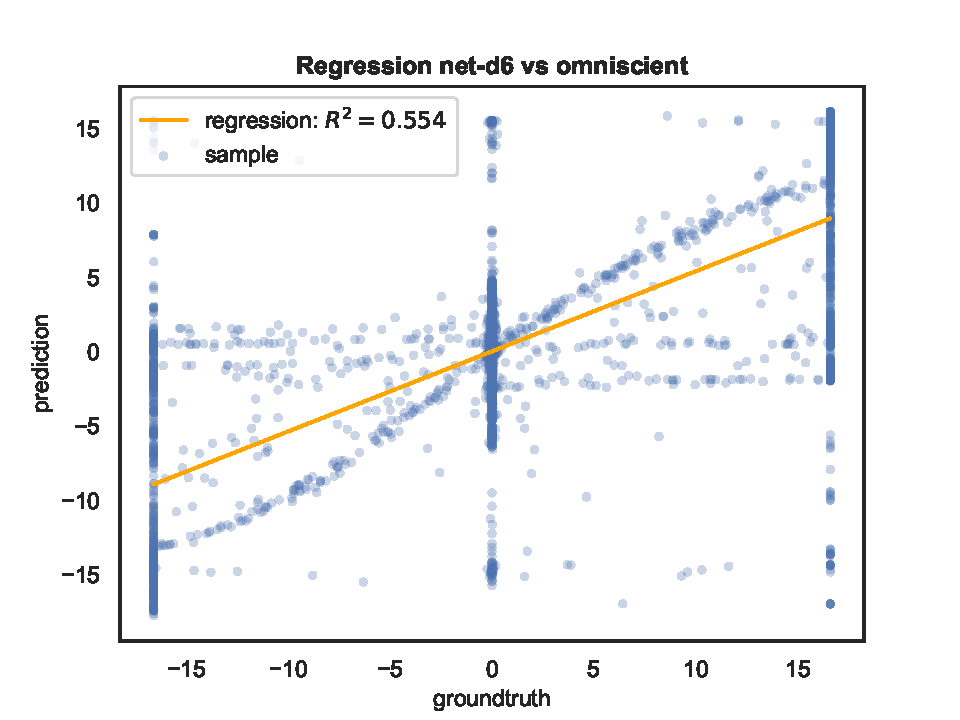
\includegraphics[width=\textwidth]{contents/images/net-d6/regression-net-d6-vs-omniscient}%
		\end{subfigure}
		\hfill\vspace{-0.5cm}
		\begin{subfigure}[h]{0.49\textwidth}
			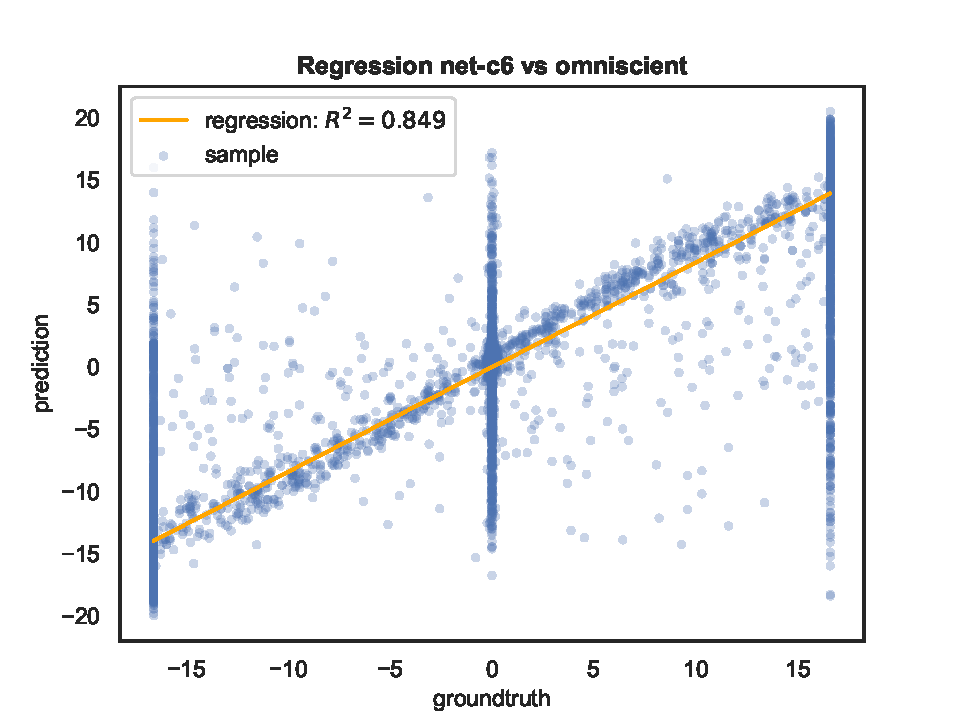
\includegraphics[width=\textwidth]{contents/images/net-c6/regression-net-c6-vs-omniscient}%
		\end{subfigure}
	\end{center}
	\caption[Evaluation of the \gls{r2} coefficients of \texttt{net-c6}.]{Comparison 
	of the \gls{r2} coefficients of the controllers learned from \texttt{net-d6} and 
	\texttt{net-c6}, with respect to the omniscient one.}
	\label{fig:net-c6r2}
\end{figure}

\begin{figure}[!htb]
	\begin{center}
		\begin{subfigure}[h]{0.49\textwidth}
			\centering
			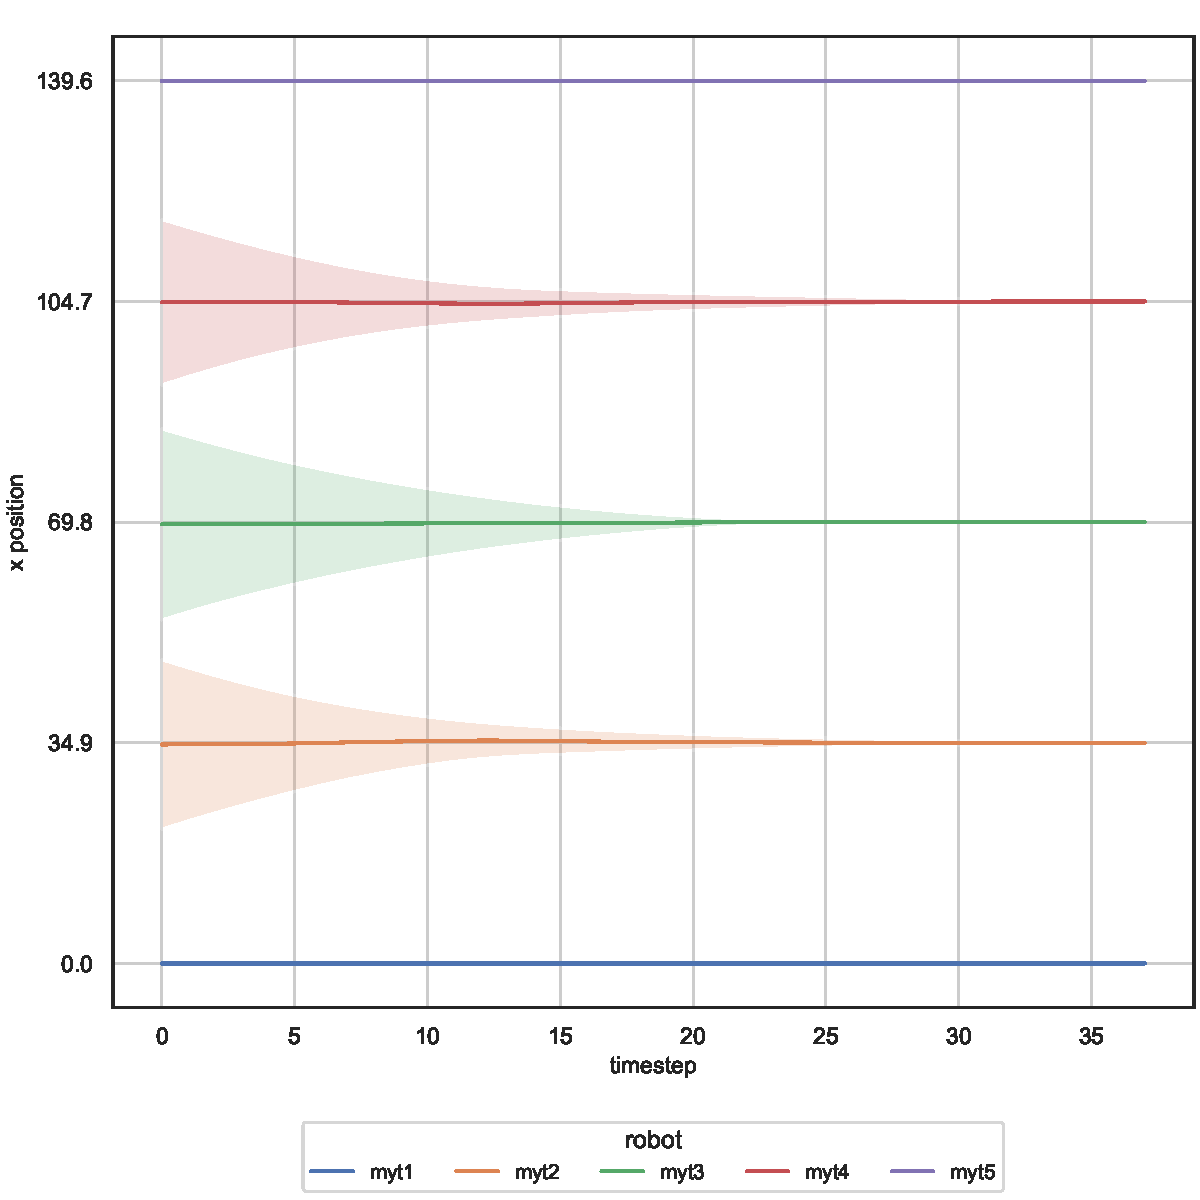
\includegraphics[width=.9\textwidth]{contents/images/net-d6/position-overtime-omniscient}%
			\caption{Expert controller trajectories.}
		\end{subfigure}
		\hfill
		\begin{subfigure}[h]{0.49\textwidth}
			\centering
			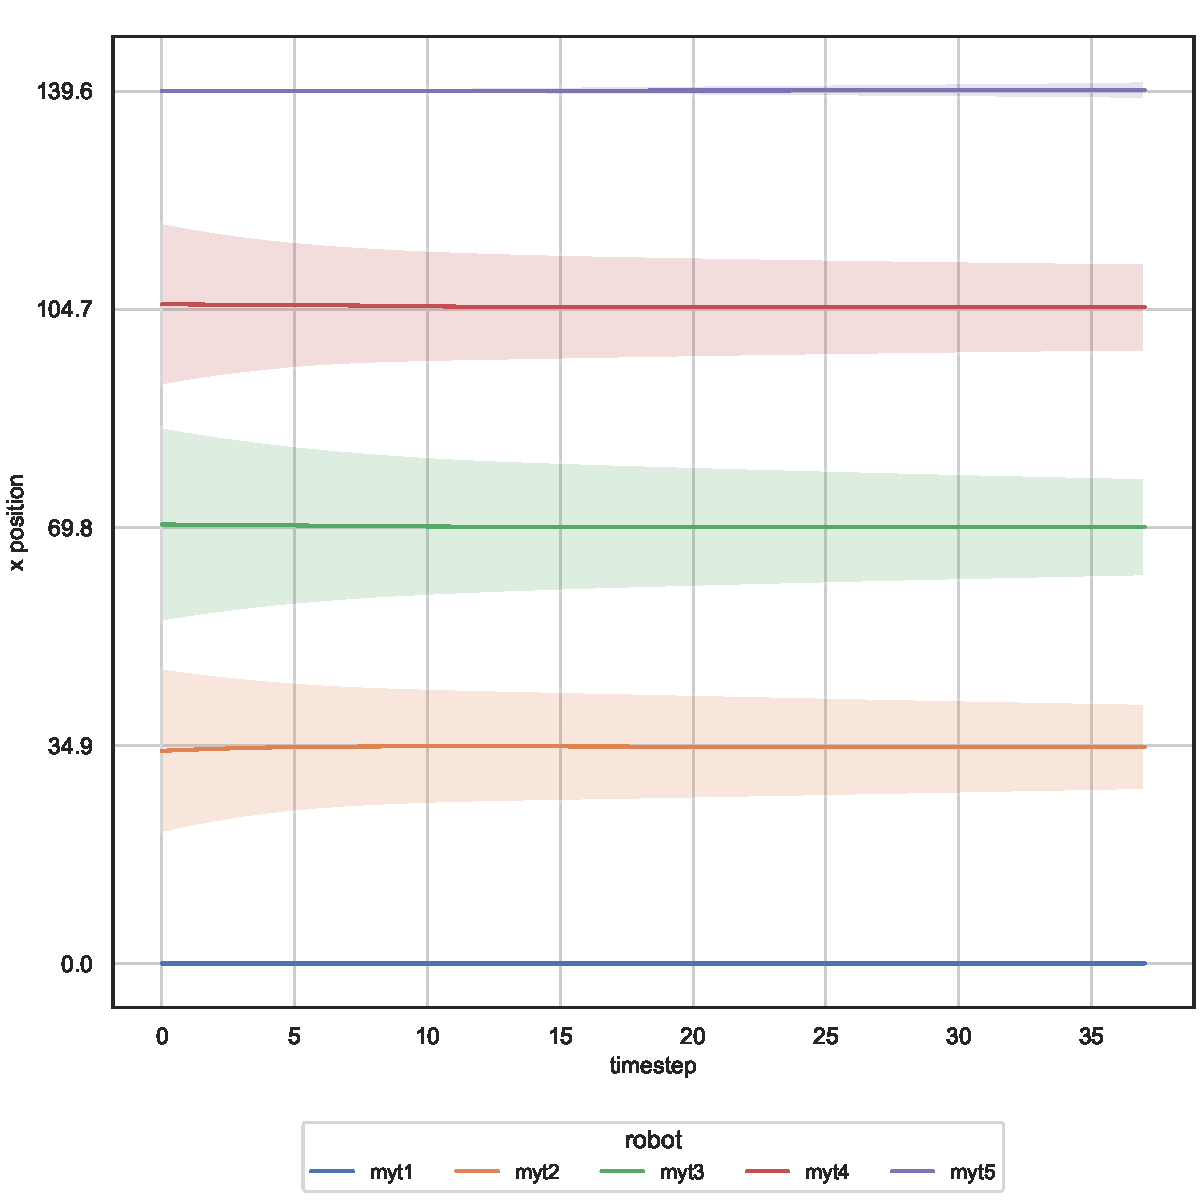
\includegraphics[width=.9\textwidth]{contents/images/net-d6/position-overtime-learned_distributed}
			\caption{Distributed controller trajectories.}
		\end{subfigure}
	\end{center}
	\vspace{-0.5cm}
	\caption[Evaluation of the trajectories learned by \texttt{net-c6}.]{Comparison 
		of trajectories generated using four controllers: the expert, the manual and 
		the two learned from \texttt{net-d6} and \texttt{net-c6}.}	
\end{figure}

\medskip
\begin{figure}[!htb]\ContinuedFloat
	\begin{center}
		\begin{subfigure}[h]{0.49\textwidth}
			\centering			
			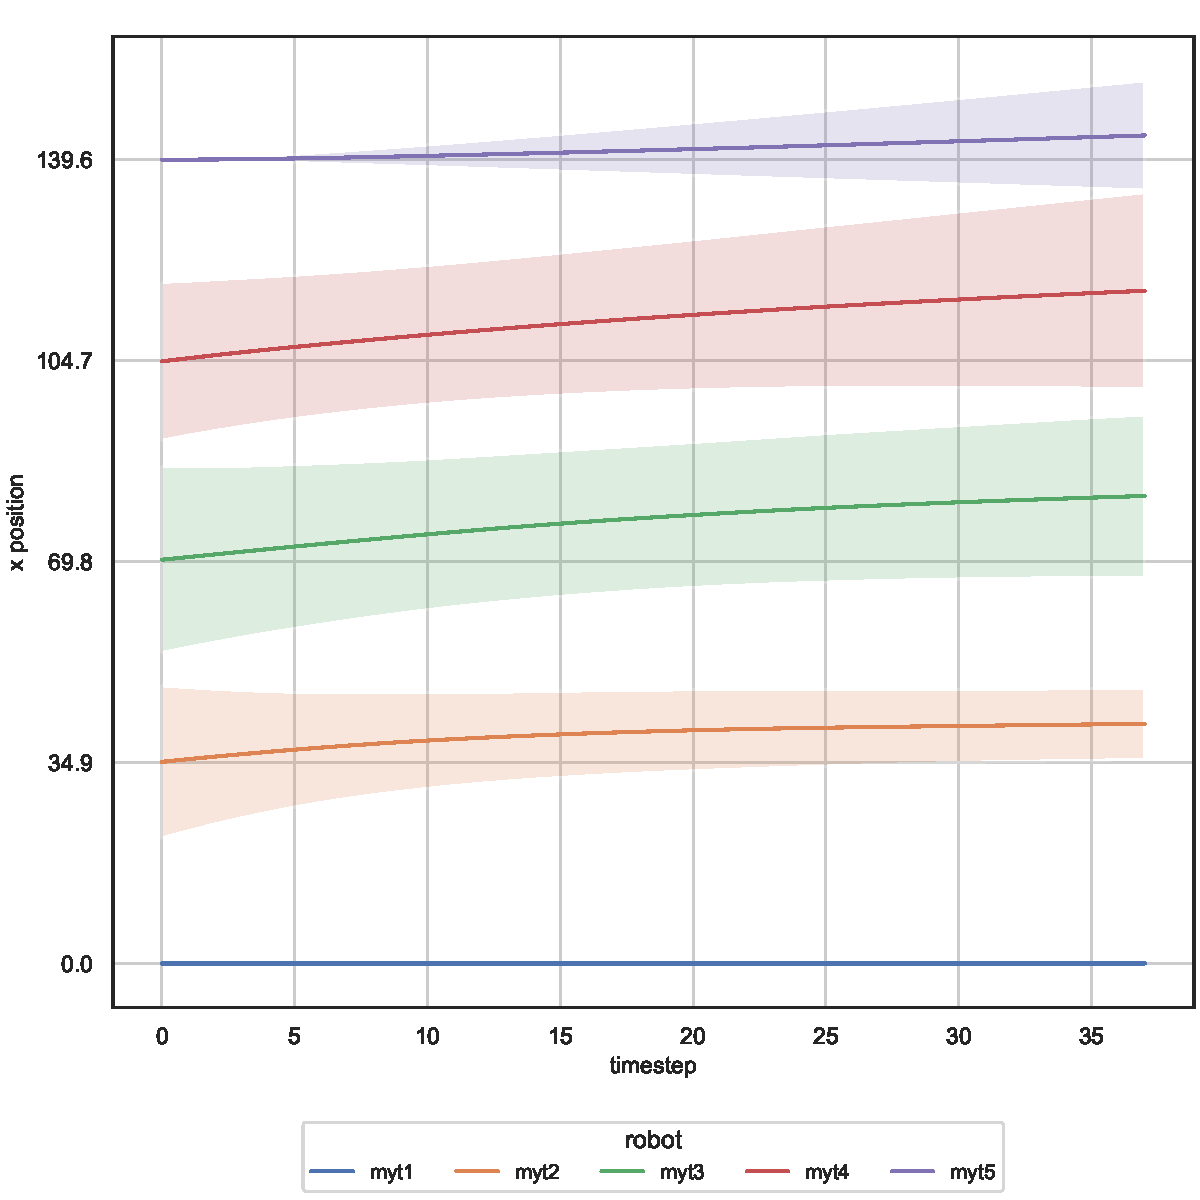
\includegraphics[width=.9\textwidth]{contents/images/net-d6/position-overtime-manual}%
			\caption{Manual controller trajectories.}
		\end{subfigure}
		\hfill
		\begin{subfigure}[h]{0.49\textwidth}
			\centering
			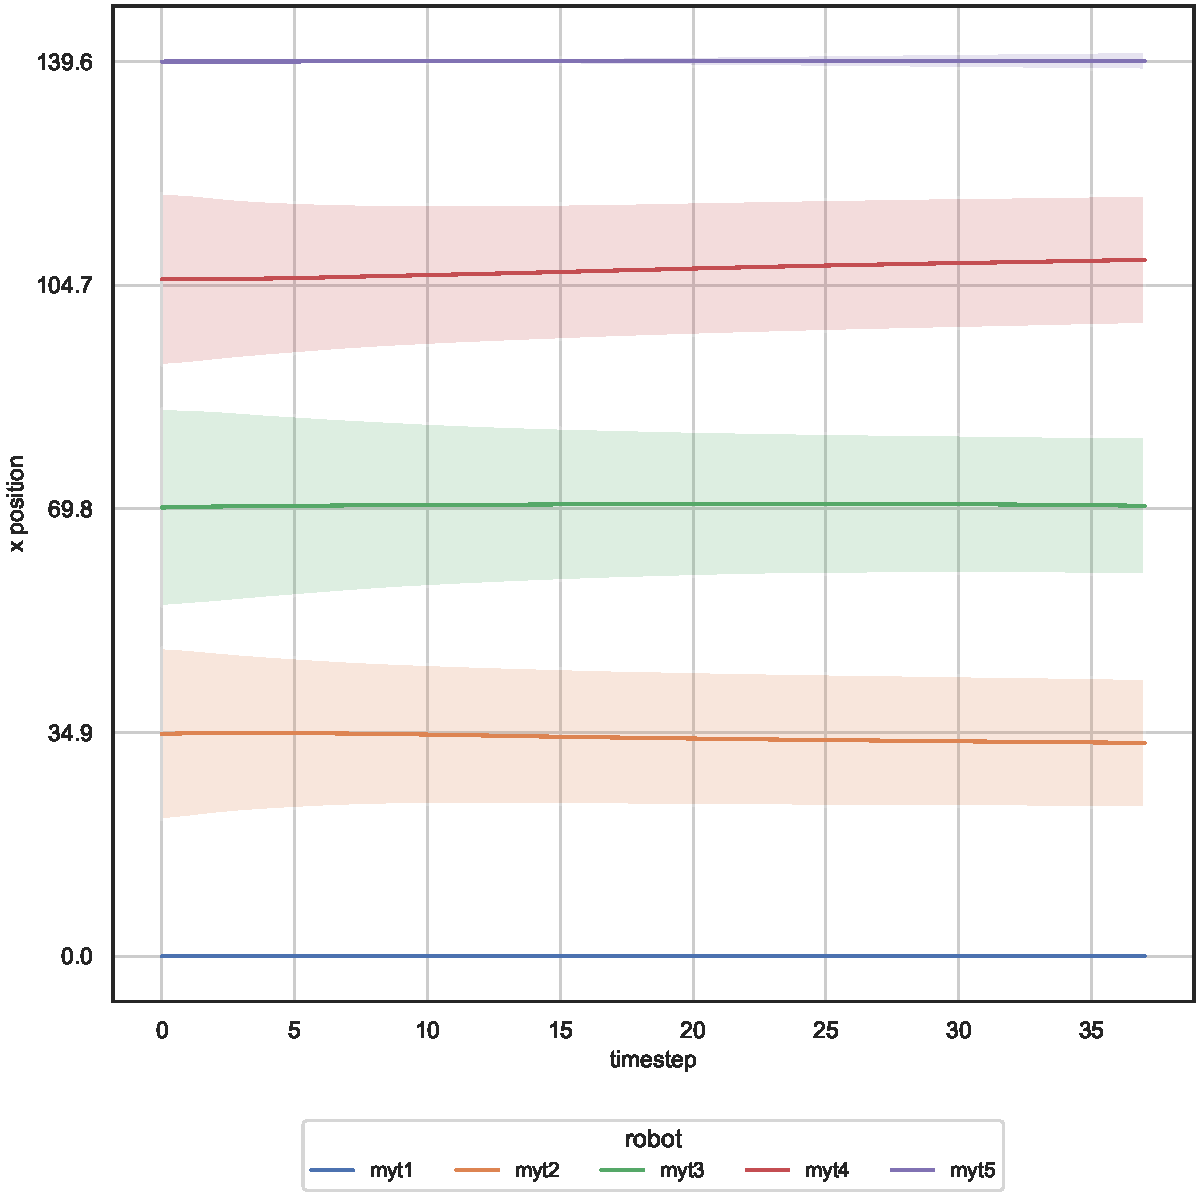
\includegraphics[width=.9\textwidth]{contents/images/net-c6/position-overtime-learned_communication}
			\caption{Communication controller trajectories.}
		\end{subfigure}
	\end{center}
	\vspace{-0.5cm}
	\caption[]{Comparison of trajectories generated using four controllers: the 
	expert, the manual and the two learned from \texttt{net-d6} and 
	\texttt{net-c6} (cont.).}
	\label{fig:net-c6traj}
\end{figure}
In Figure \ref{fig:net-c6traj} are shown the trajectories obtained employing the 
four controllers. Even for the expert, the convergence to the target is slower than 
before, as expected since the distance between the robots is greater, but it is 
much faster than with the other two controllers. As we said for figure 
\ref{fig:net-d6traj}, the manual controller has serious problems in reaching the 
goal. The two learned controllers can still try to approach the desired position 
employing more timesteps.

In addition, the analysis of the evolution of the control over time in Figure 
\ref{fig:net-c6control} suggests that the reason for this behaviour is the fact the 
both the learned controllers use a lower speed than expected.
\begin{figure}[!htb]
	\begin{center}
		\begin{subfigure}[h]{0.35\textwidth}
			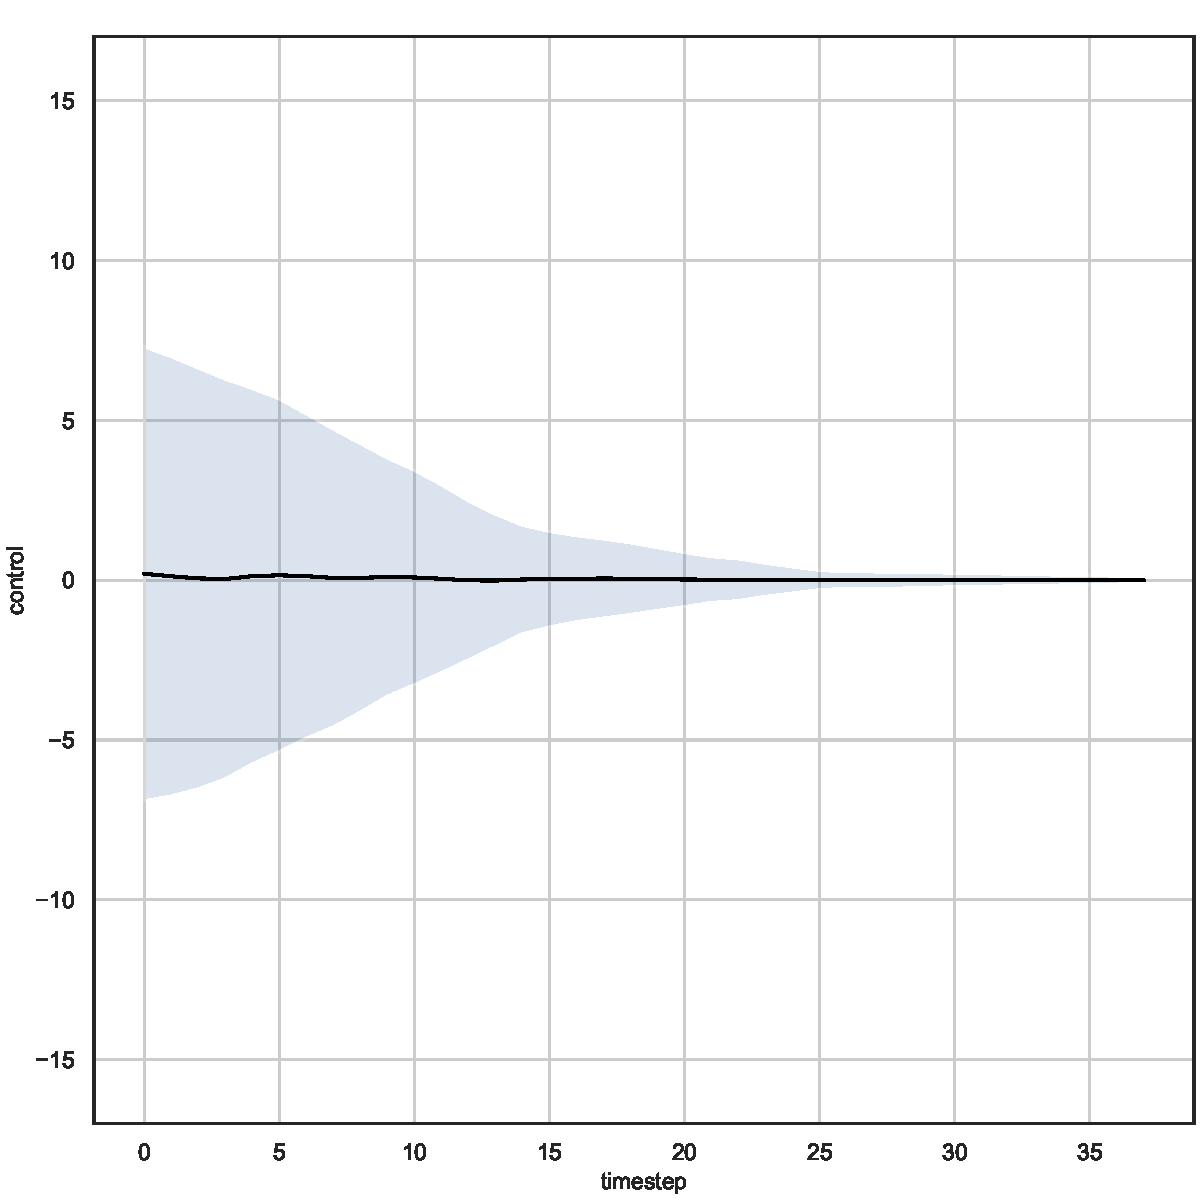
\includegraphics[width=\textwidth]{contents/images/net-d6/control-overtime-omniscient}%
			\caption{Expert control.}
		\end{subfigure}
		\hspace{1cm}
		\begin{subfigure}[h]{0.35\textwidth}
			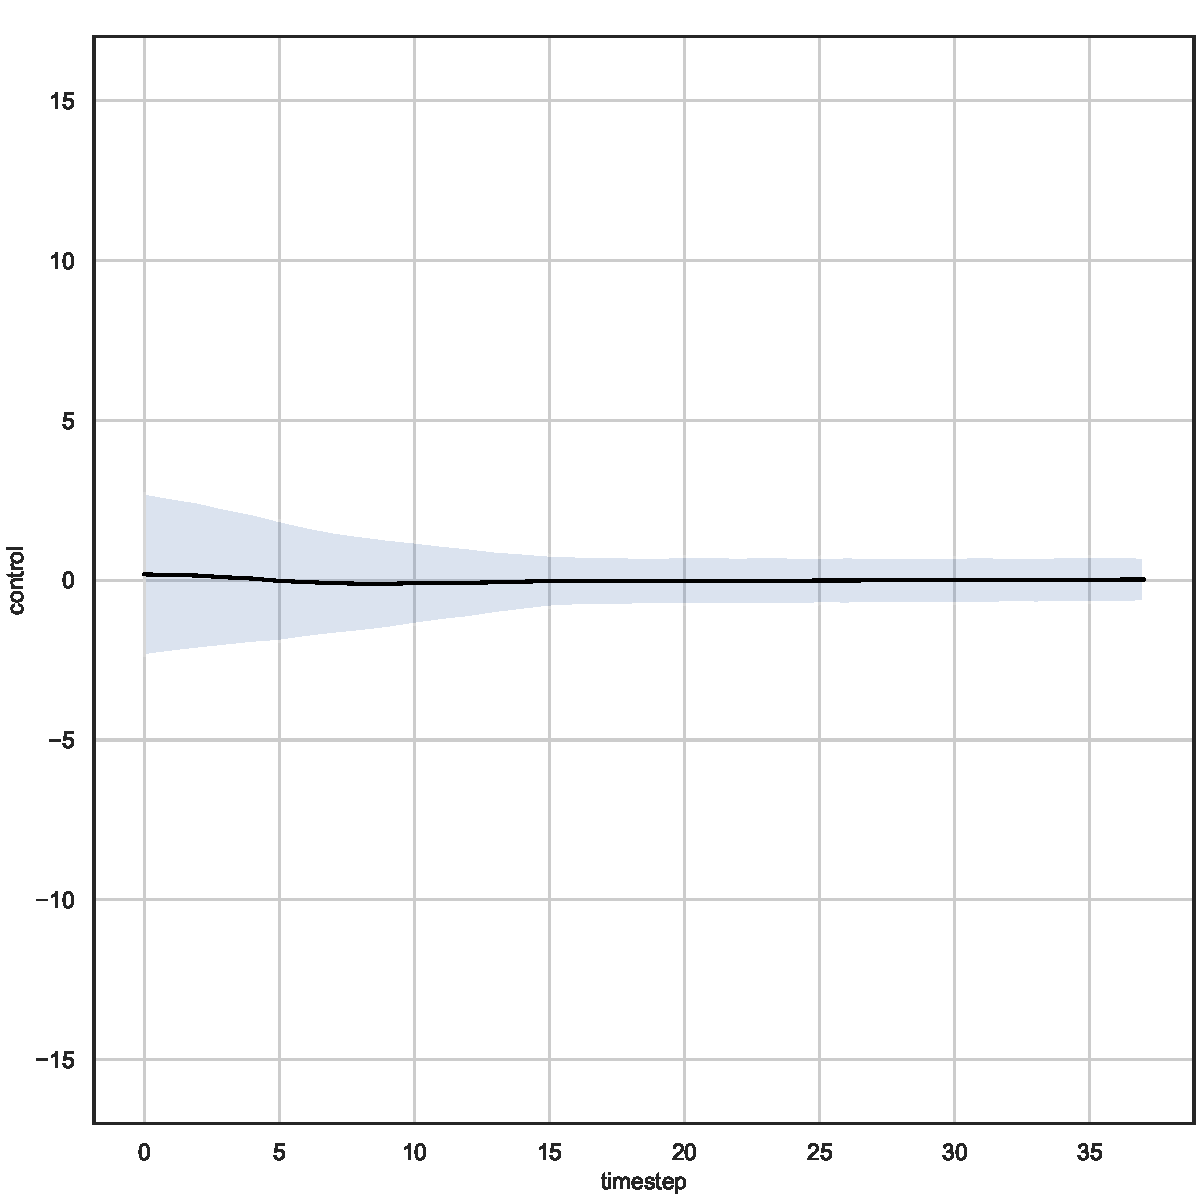
\includegraphics[width=\textwidth]{contents/images/net-d6/control-overtime-learned_distributed}
			\caption{Distributed control.}
		\end{subfigure}
	\end{center}
	\vspace{-0.5cm}
	\caption[Evaluation of the control decided by \texttt{net-c6}.]{Comparison of 
	output control decided using four controllers: the expert, the manual and the 
	two learned from \texttt{net-d6} and \texttt{net-c6}.}
\end{figure}

\medskip
\begin{figure}[!htb]\ContinuedFloat
	\begin{center}
		\begin{subfigure}[h]{0.35\textwidth}			
			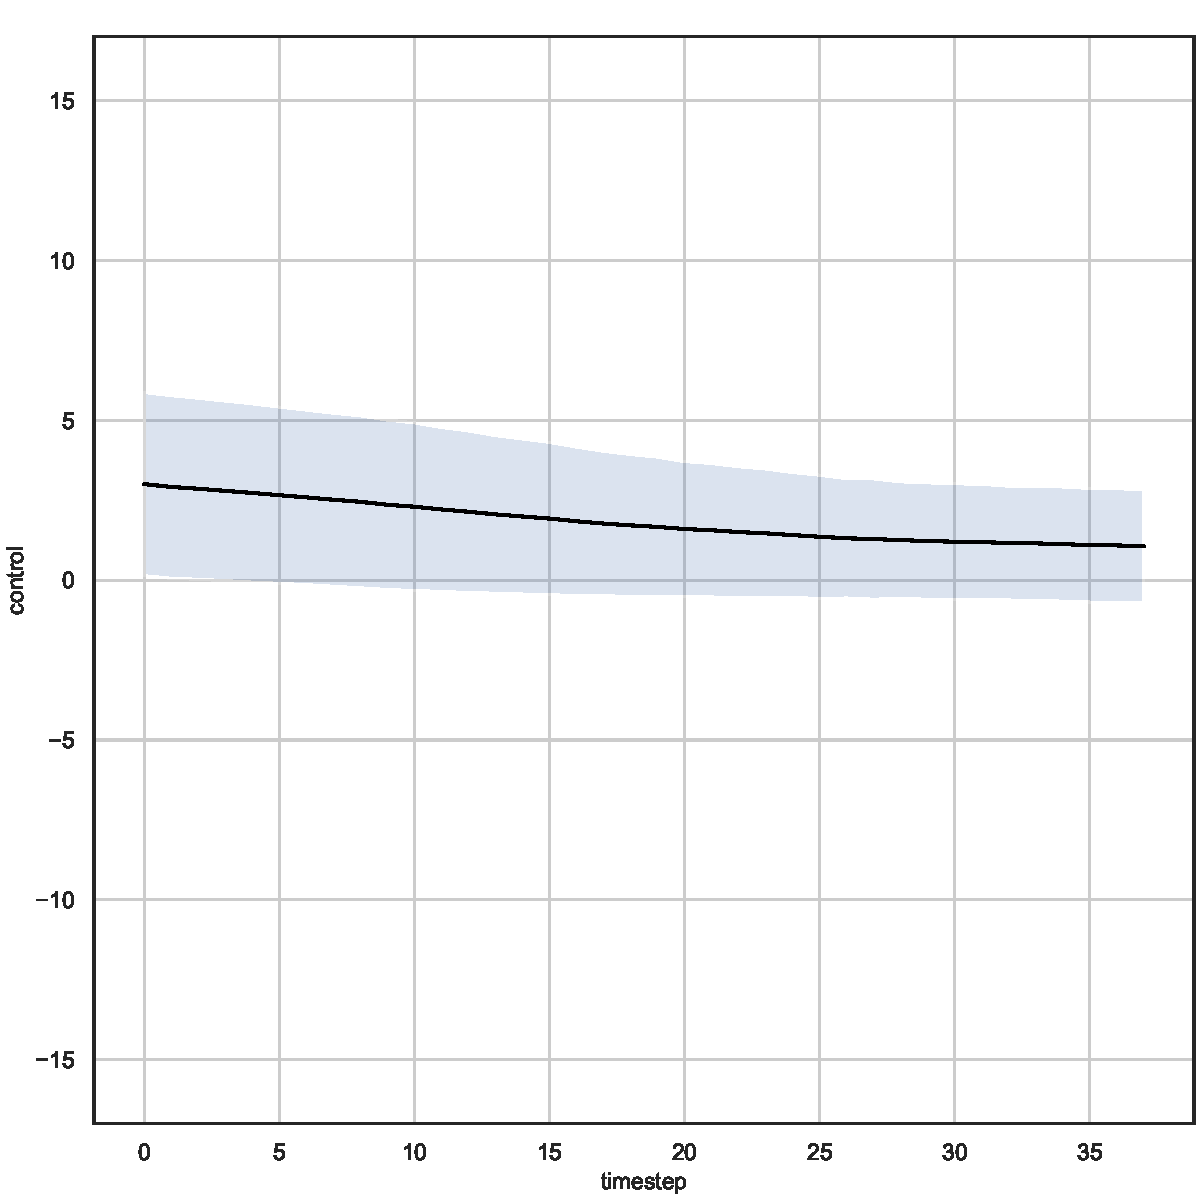
\includegraphics[width=\textwidth]{contents/images/net-d6/control-overtime-manual}%
			\caption{Manual control.}
		\end{subfigure}
		\hspace{1cm}
		\begin{subfigure}[h]{0.35\textwidth}
			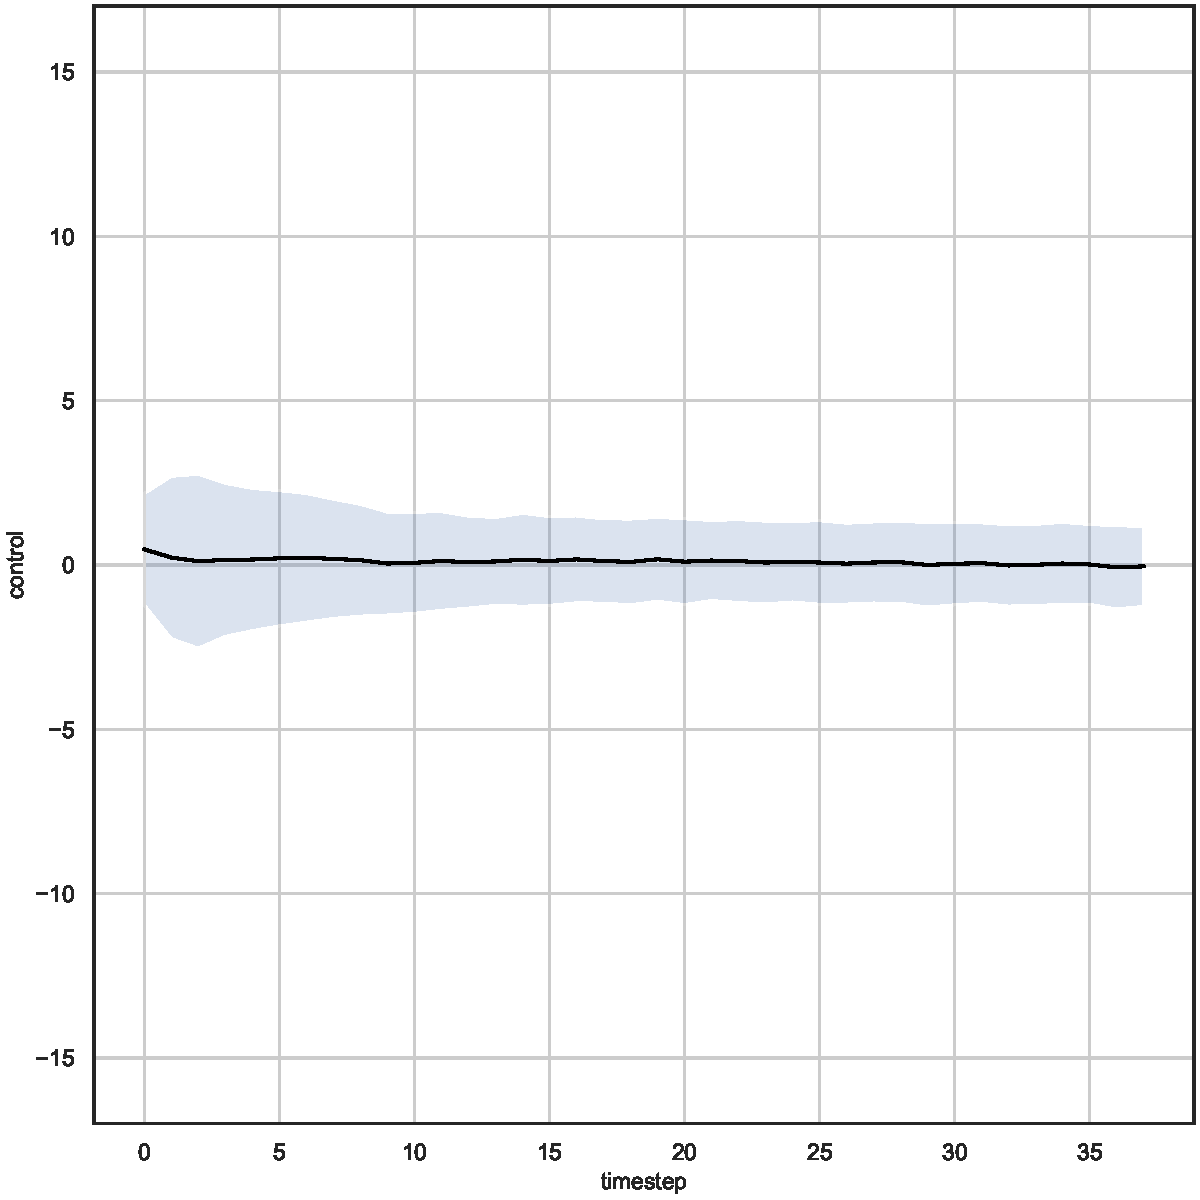
\includegraphics[width=\textwidth]{contents/images/net-c6/control-overtime-learned_communication}
			\caption{Communication control.}
		\end{subfigure}
	\end{center}
	\vspace{-0.5cm}
	\caption{Comparison of output control decided using four controllers: the 
	expert, the manual and the two learned from \texttt{net-d6} and 
	\texttt{net-c6} (cont.).}
	\label{fig:net-c6control}
\end{figure}

In Figure \ref{fig:net-c6responseposition} is displayed the behaviour of a robot 
located between two stationary agents, showing the response of the controllers, 
on the y-axis, by varying the position of the moving robot, visualised on the 
x-axis.  
\begin{figure}[!htb]
	\centering
	\includegraphics[width=.45\textwidth]{contents/images/net-c6/response-varying_init_position-communication}%
	\caption{Response of \texttt{net-c6} by varying the initial position.}
	\label{fig:net-c6responseposition}
\end{figure}
As expected, the output is a high positive value when the robot is close to an 
obstacle on the left, negative when there is an obstacle in front and not behind, 
and $0$ when the distance from right and left is equal.
The behaviour of the controller that uses the communication is the most accurate 
when the moving robot is halfway between the two stationary.

Finally, in Figure \ref{fig:net-c6distance} is presented a metric that measures the 
absolute distance of each robot from the target over time.
Unlike the non-optimal performances obtained with the manual and distributed 
controllers, in which in both cases the robots in the final configuration are 
located on average at about $5$\gls{cm} from the target, the distance from goal 
of the communication controller is far better. In just $11$ time steps, $4$ more 
than the expert, the agents reach the goal position.
\begin{figure}[H]
	\centering
	\includegraphics[width=.65\textwidth]{contents/images/net-c6/distances-from-goal-compressed-communication}%
	\caption[Evaluation of \texttt{net-c6} distances from goal.]{Comparison of 
		performance in terms of distances from goal obtained using four controllers: 
		the expert, the manual and the two learned from \texttt{net-d6} and 
		\texttt{net-c6}.}
	\label{fig:net-c6distance}
\end{figure}

As before, is very difficult to analyse the communication transmitted over time 
through the visualisation in Figure \ref{fig:net-c6comm}. In this case, the agents 
seem to communicate initially a high value  that is decrease by approaching the 
final configuration.
\begin{figure}[!htb]
	\centering
	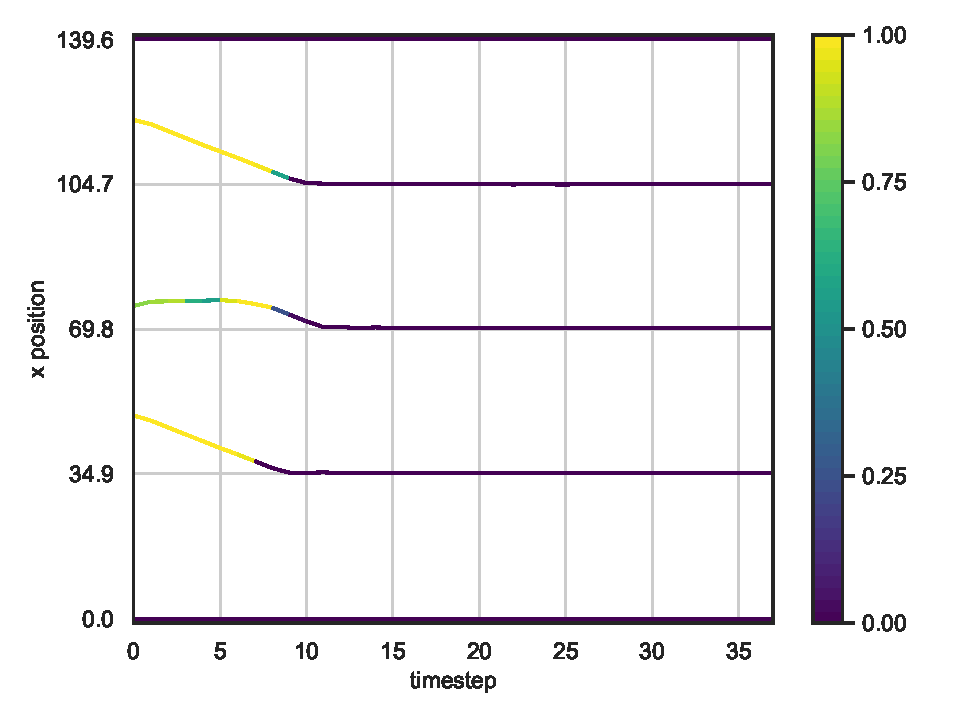
\includegraphics[width=.65\textwidth]{contents/images/net-c6/4/plot-simulation-communication-4}
	\vspace{-0.5cm}
	\caption[Evaluation of the communication learned by 
	\texttt{net-c6}.]{Visualisation of the communication values transmitted by each 
		robot over time using the controller learned from \texttt{net-c6}.}	
	\label{fig:net-c6comm}
\end{figure}

We conclude the first group of experiments presenting the results obtained using 
both types of input together from which we expect a more stable and robust 
behaviour.

In Figure \ref{fig:commlossall_sensors} are summarised the performance, 
in terms of loss, of the models trained using \texttt{all\_sensors} input and 
different gaps: the blue, orange and green lines represent respectively average 
gaps of $8$, $13$ and $24$\gls{cm}.
It is immediately evident that using the new approach the trend of the curves are 
very similar to each other, and in general the loss is considerably decreased down 
to $20$.
\begin{figure}[!htb]
	\begin{center}
			\begin{subfigure}[h]{0.49\textwidth}
			\centering
			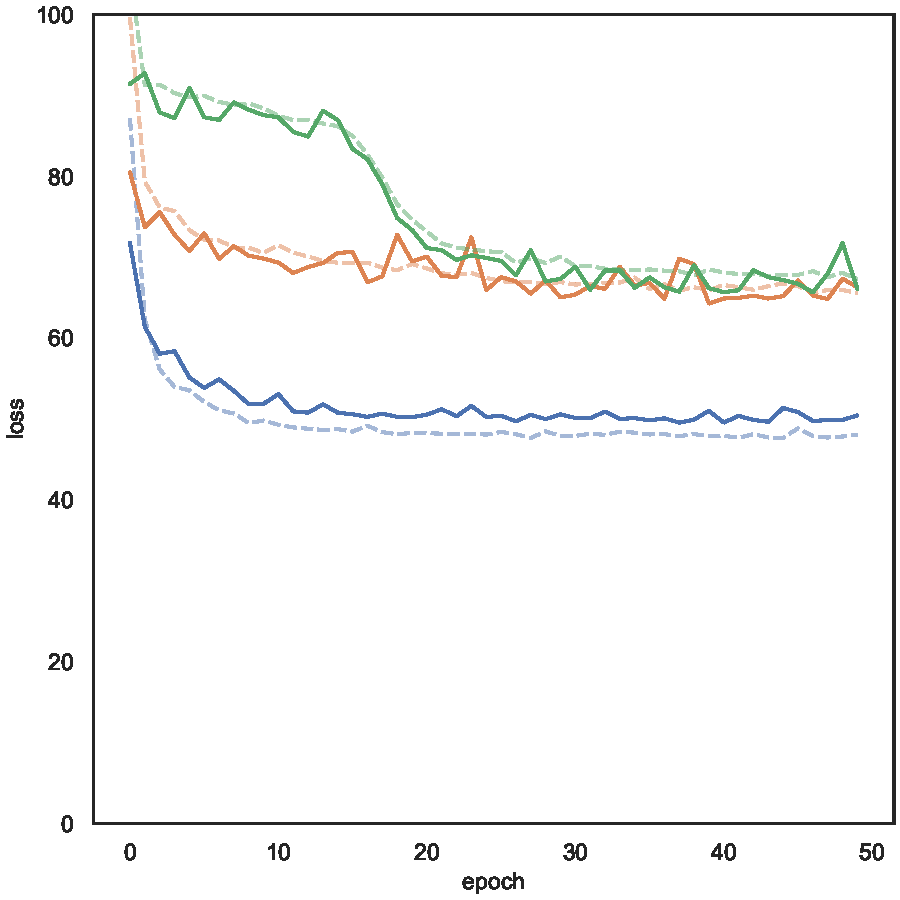
\includegraphics[width=.7\textwidth]{contents/images/task1-comm/loss-distributed-all_sensors@copy}
			\caption{Distributed approach.}
		\end{subfigure}
		\hfill
		\begin{subfigure}[h]{0.49\textwidth}
			\centering
			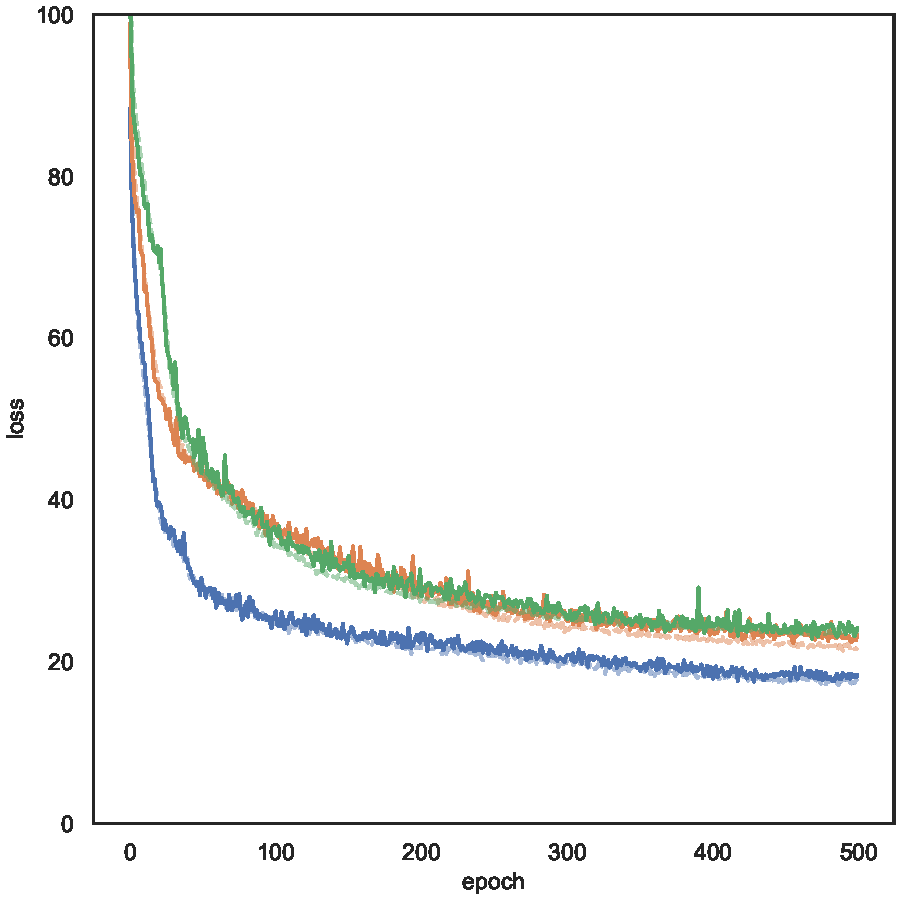
\includegraphics[width=.7\textwidth]{contents/images/task1-comm/loss-communication-all_sensors@copy}
			\caption{Distributed approach with communication.}
		\end{subfigure}	
	\end{center}
	\vspace{-0.5cm}
	\caption{Comparison of the losses of the models that use \texttt{all\_sensors} 
		readings.}
	\label{fig:commlossall_sensors}
\end{figure}

Considering as before the more complex case, for instance the one with the 
greatest average gap, in Figure \ref{fig:net-c9r2} are visualised the \gls{r2} of the 
manual and the learned controllers, with and without communication.
The superiority of the new approach is once again confirmed by the increase in 
the coefficient \gls{r2} from $0.56$ to $0.84$. 
\begin{figure}[!htb]
	\begin{center}
		\begin{subfigure}[h]{0.49\textwidth}
			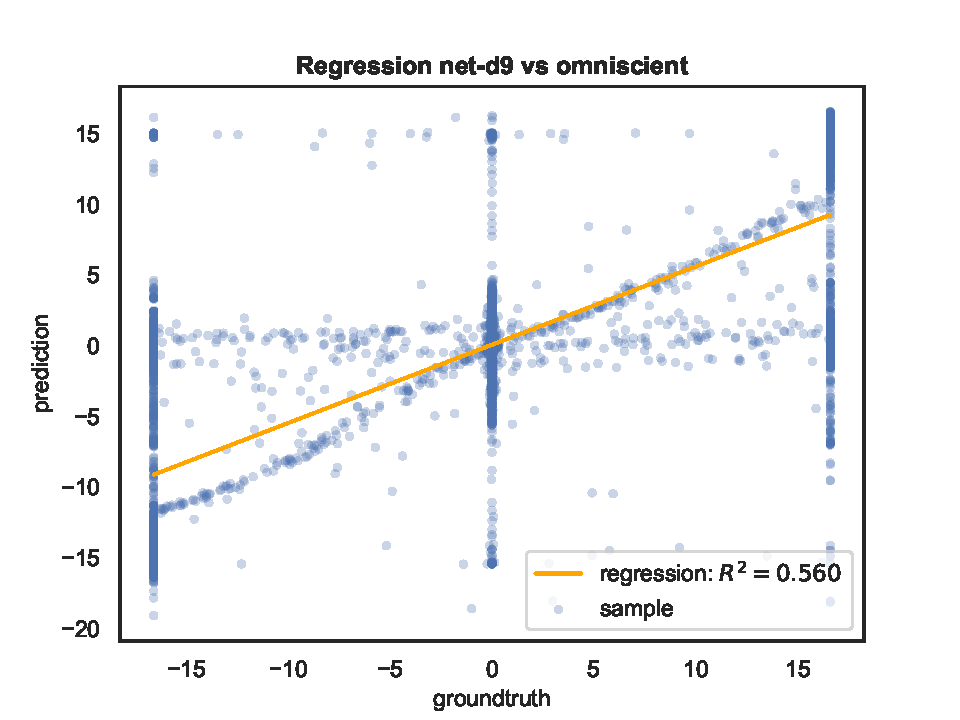
\includegraphics[width=\textwidth]{contents/images/net-d9/regression-net-d9-vs-omniscient}%
		\end{subfigure}
		\hfill\vspace{-0.5cm}
		\begin{subfigure}[h]{0.49\textwidth}
			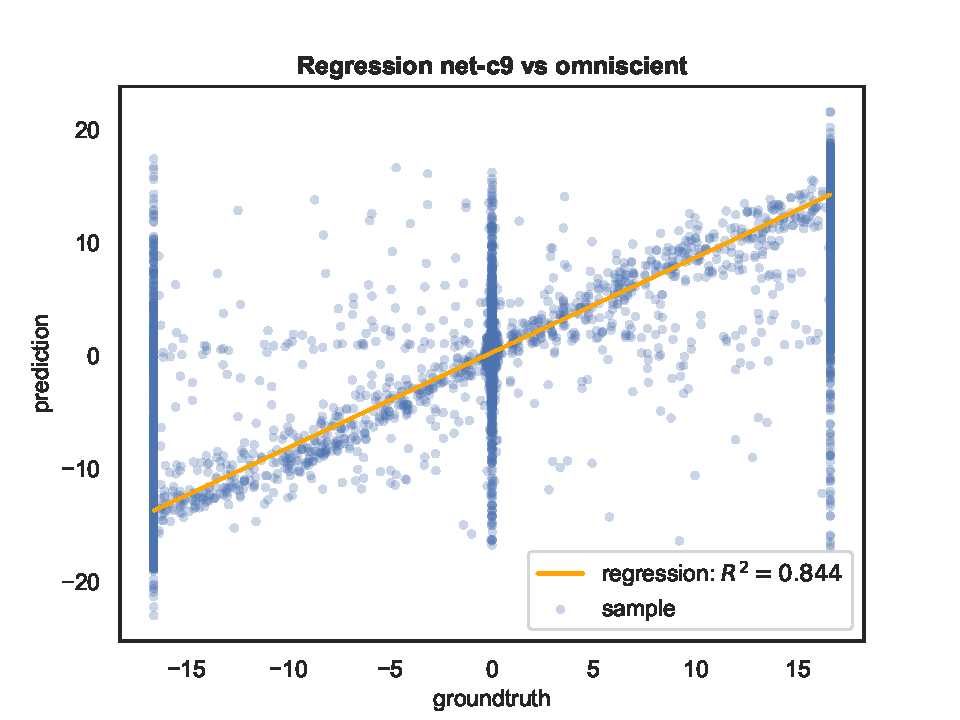
\includegraphics[width=\textwidth]{contents/images/net-c9/regression-net-c9-vs-omniscient}%
		\end{subfigure}
	\end{center}
	\caption[Evaluation of the \gls{r2} coefficients of \texttt{net-c9}.]{Comparison 
		of the \gls{r2} coefficients of the controllers learned from 
		\texttt{net-d9} and \texttt{net-c9}, with respect to the omniscient one.}
	\label{fig:net-c9r2}
\end{figure}

\begin{figure}[!htb]
	\begin{center}
		\begin{subfigure}[h]{0.49\textwidth}
			\centering
			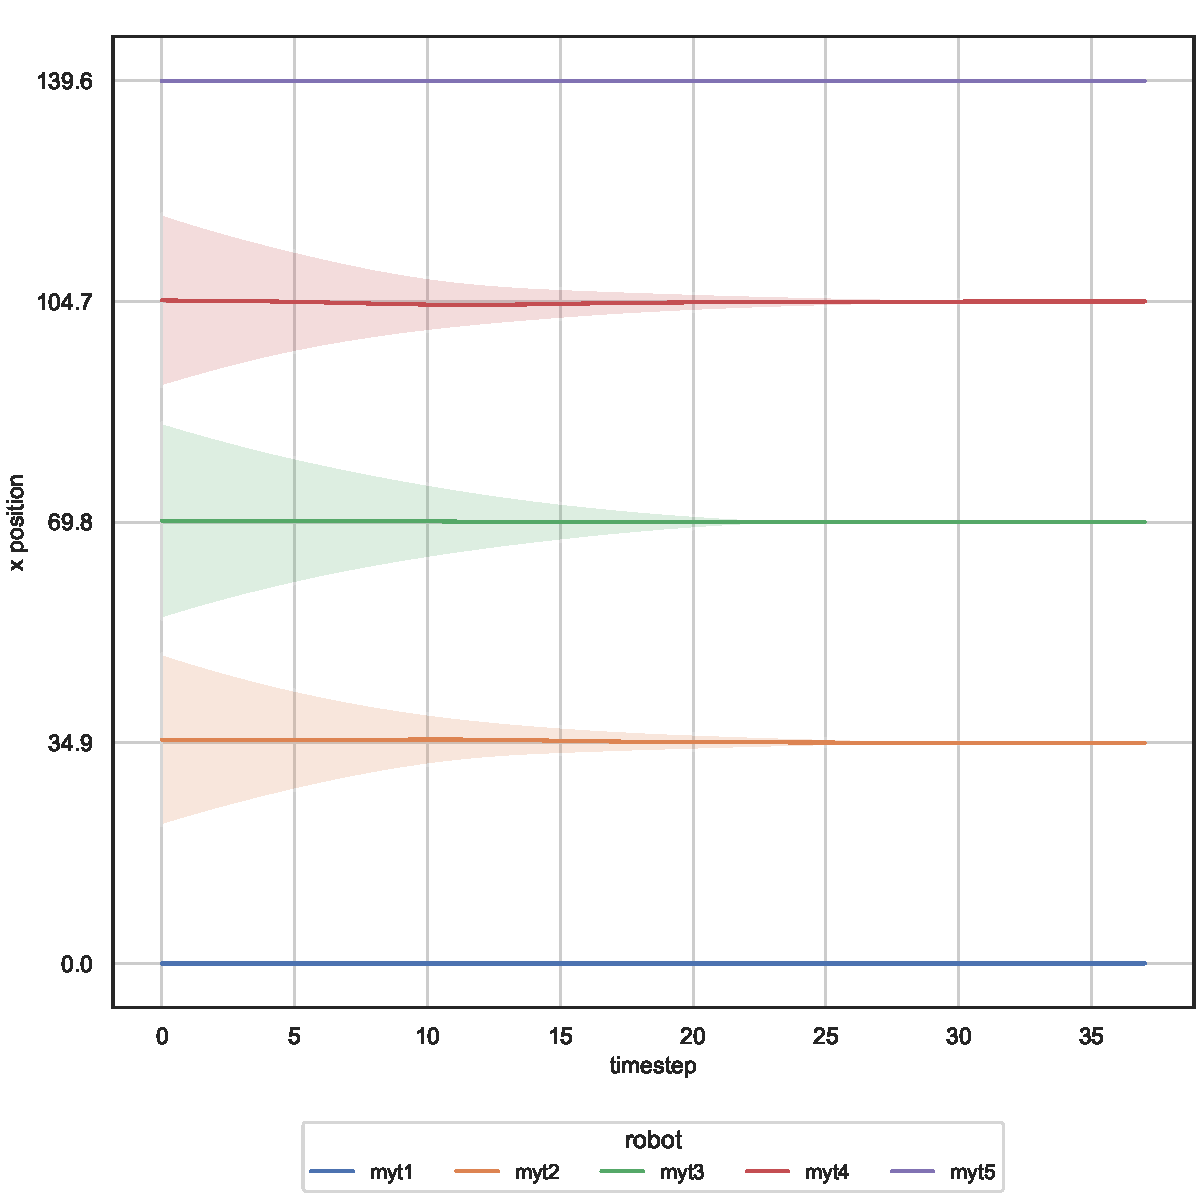
\includegraphics[width=.9\textwidth]{contents/images/net-d9/position-overtime-omniscient}%
			\caption{Expert controller trajectories.}
		\end{subfigure}
		\hfill
		\begin{subfigure}[h]{0.49\textwidth}
			\centering
			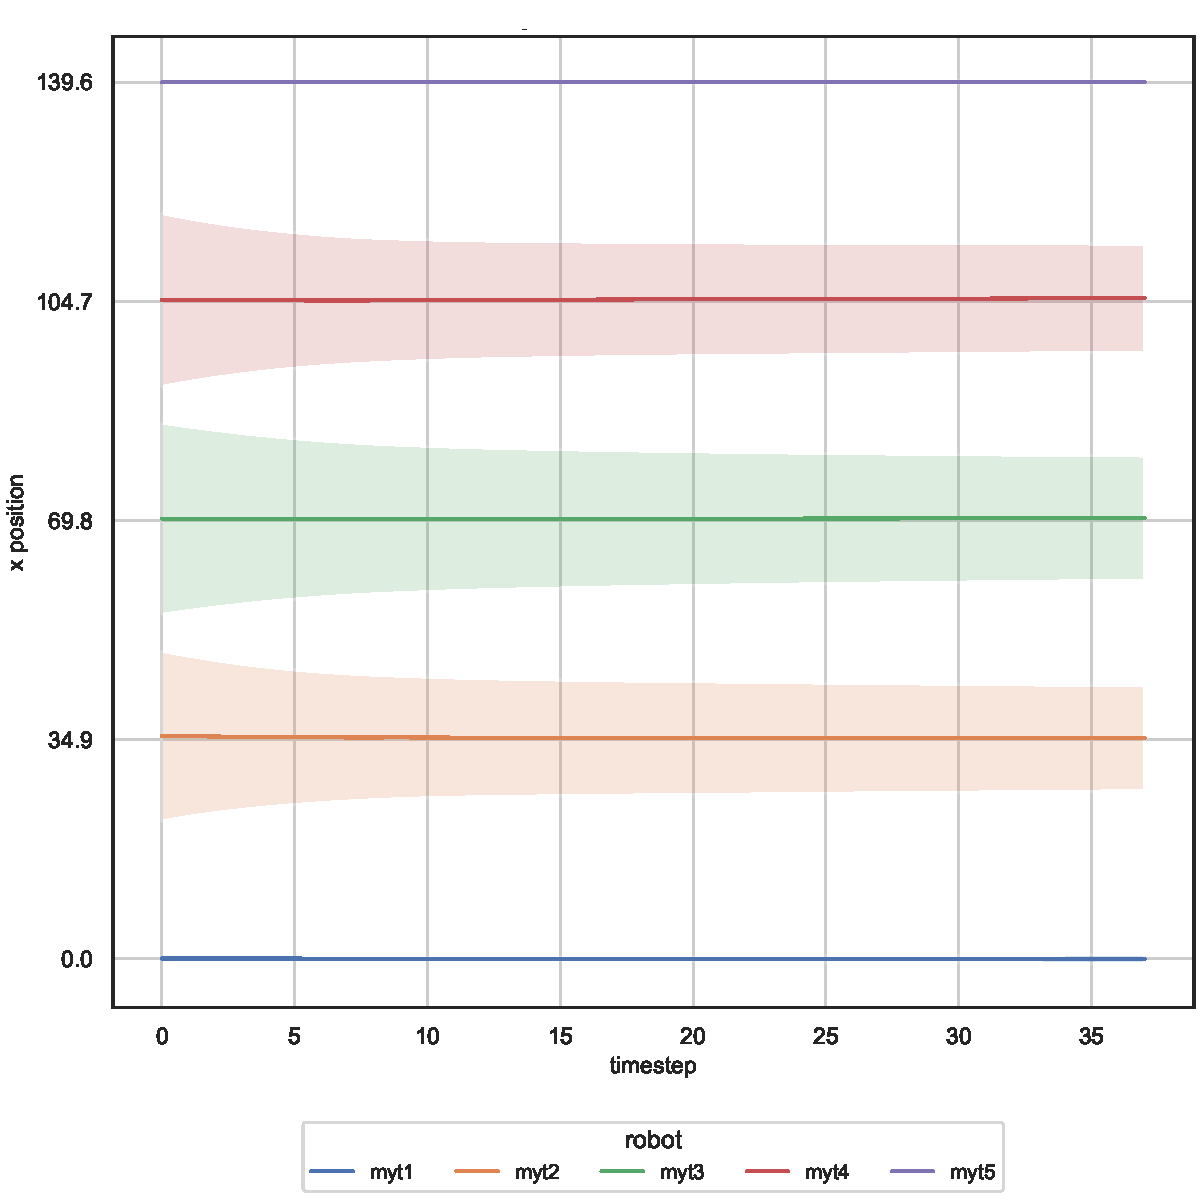
\includegraphics[width=.9\textwidth]{contents/images/net-d9/position-overtime-learned_distributed}
			\caption{Distributed controller trajectories.}
		\end{subfigure}
	\end{center}
	\begin{center}
		\begin{subfigure}[h]{0.49\textwidth}
			\centering			
			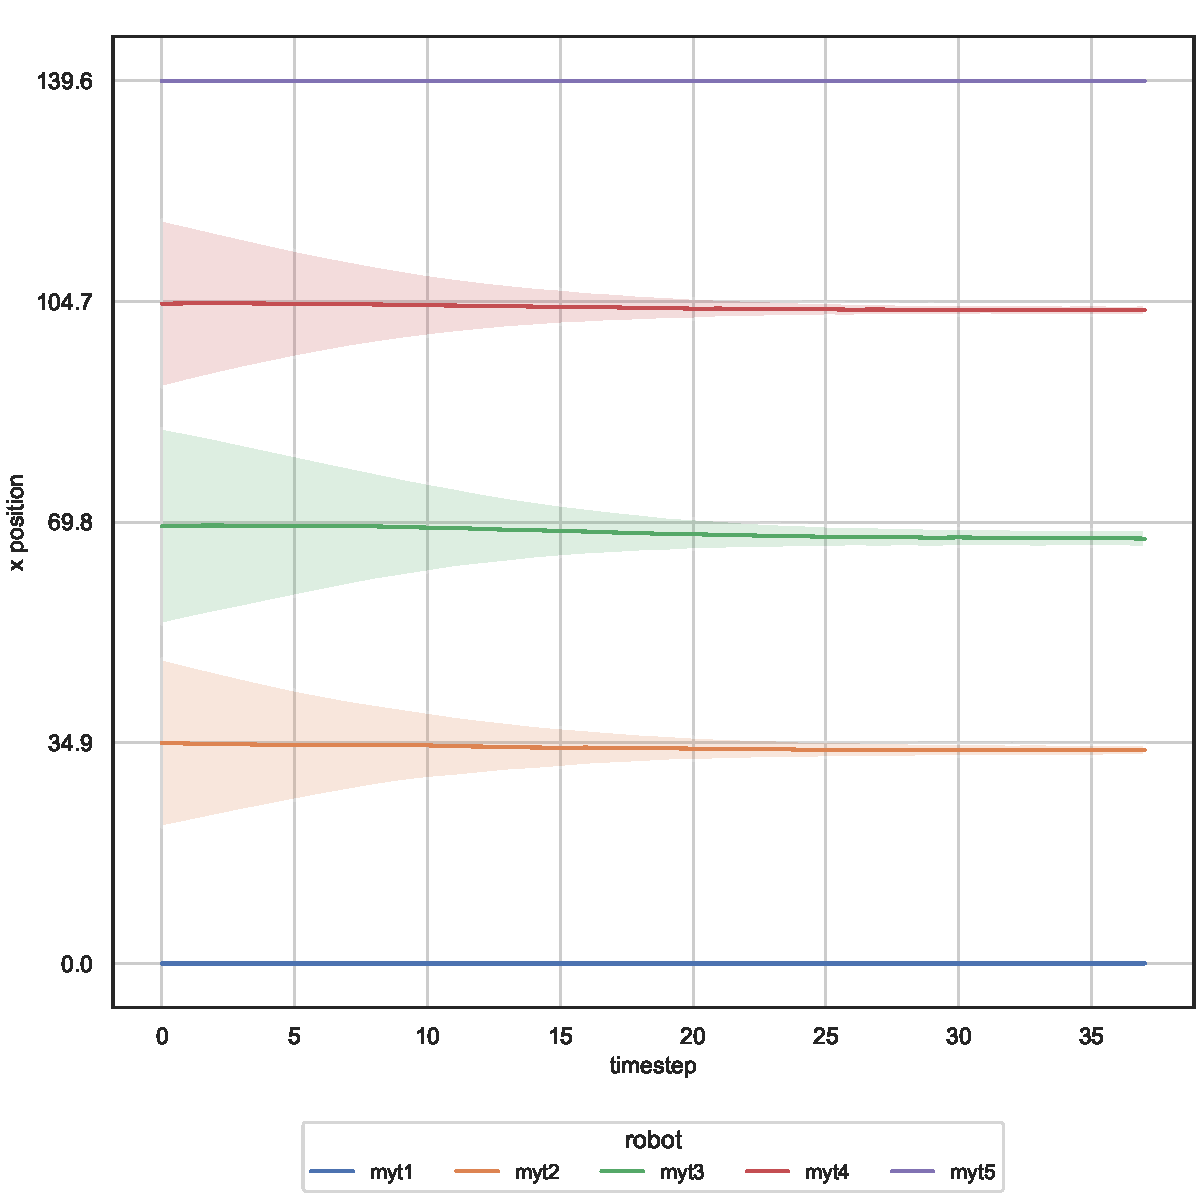
\includegraphics[width=.9\textwidth]{contents/images/net-d9/position-overtime-manual}%
			\caption{Manual controller trajectories.}
		\end{subfigure}
		\hfill
		\begin{subfigure}[h]{0.49\textwidth}
			\centering
			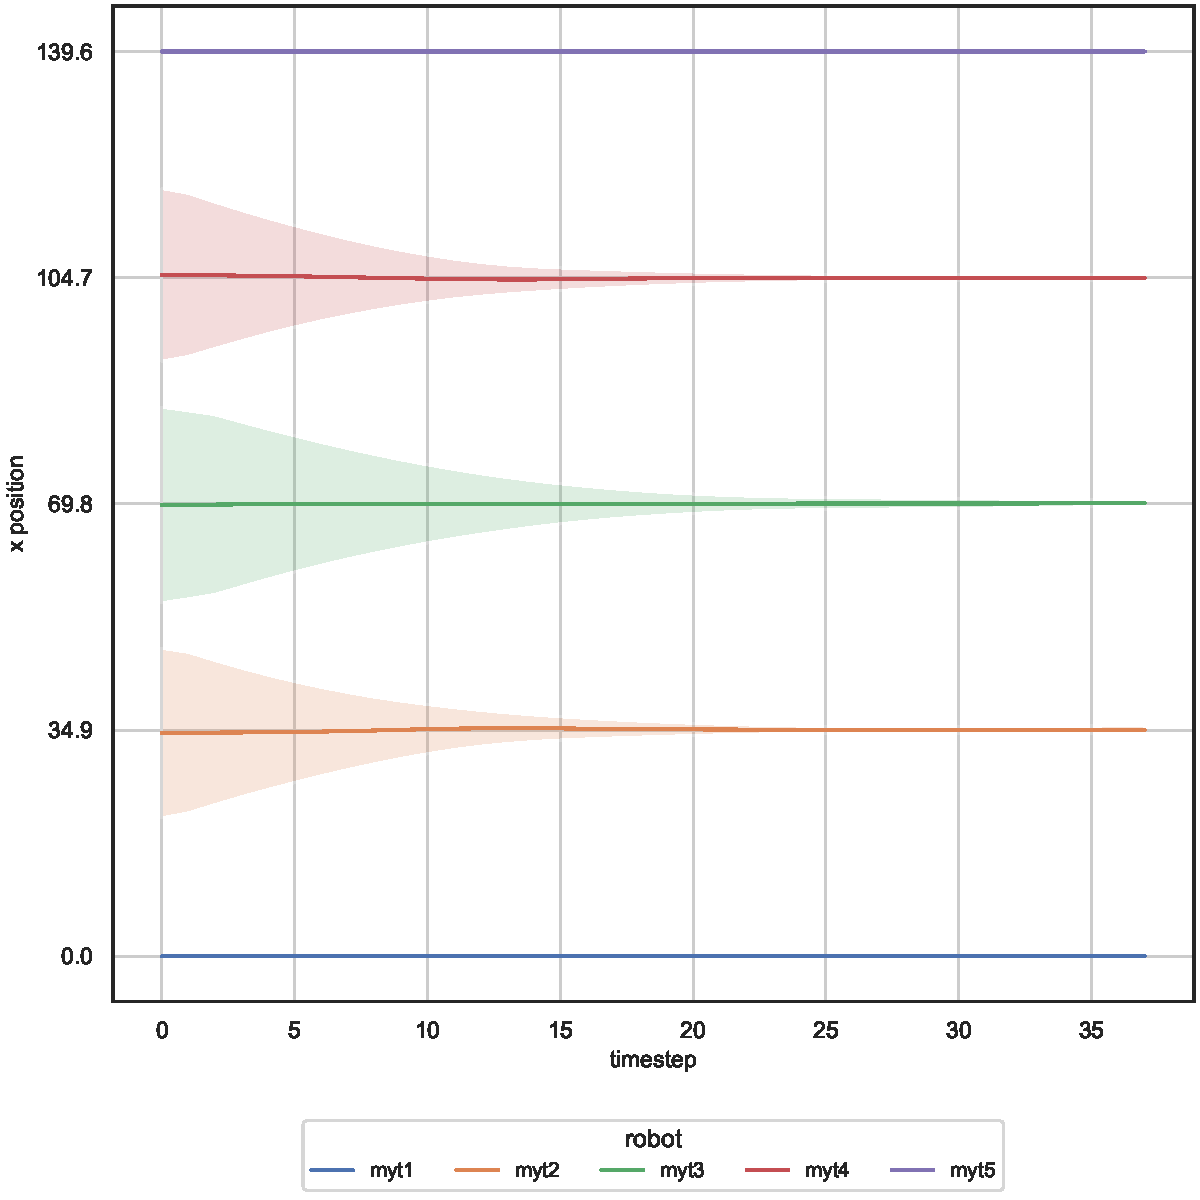
\includegraphics[width=.9\textwidth]{contents/images/net-c9/position-overtime-learned_communication}
			\caption{Communication controller trajectories.}
		\end{subfigure}
	\end{center}
	\vspace{-0.5cm}
	\caption[Evaluation of the trajectories learned by \texttt{net-c9}.]{Comparison 
	of trajectories generated using four controllers: the expert, the manual and the 
	two learned from \texttt{net-d9} and \texttt{net-c9}.}
	\label{fig:net-c9traj}
\end{figure}
This improvement is further supported by the trajectories shown in Figure 
\ref{fig:net-c9traj}. 
The convergence to the target is still slow due to the high distance between the 
robots, but this time the controller with communication is much faster than the 
distributed controller but also than the manual. The bands of the deviation show 
that this approach can reach the same results of the expert.

Moreover, analysing the evolution of the control over time in Figure 
\ref{fig:net-c9control}, we observe that this time the control learned from the 
network with communication is very similar to that decided by the omniscient 
controller.
\begin{figure}[!htb]
	\begin{center}
		\begin{subfigure}[h]{0.35\textwidth}
			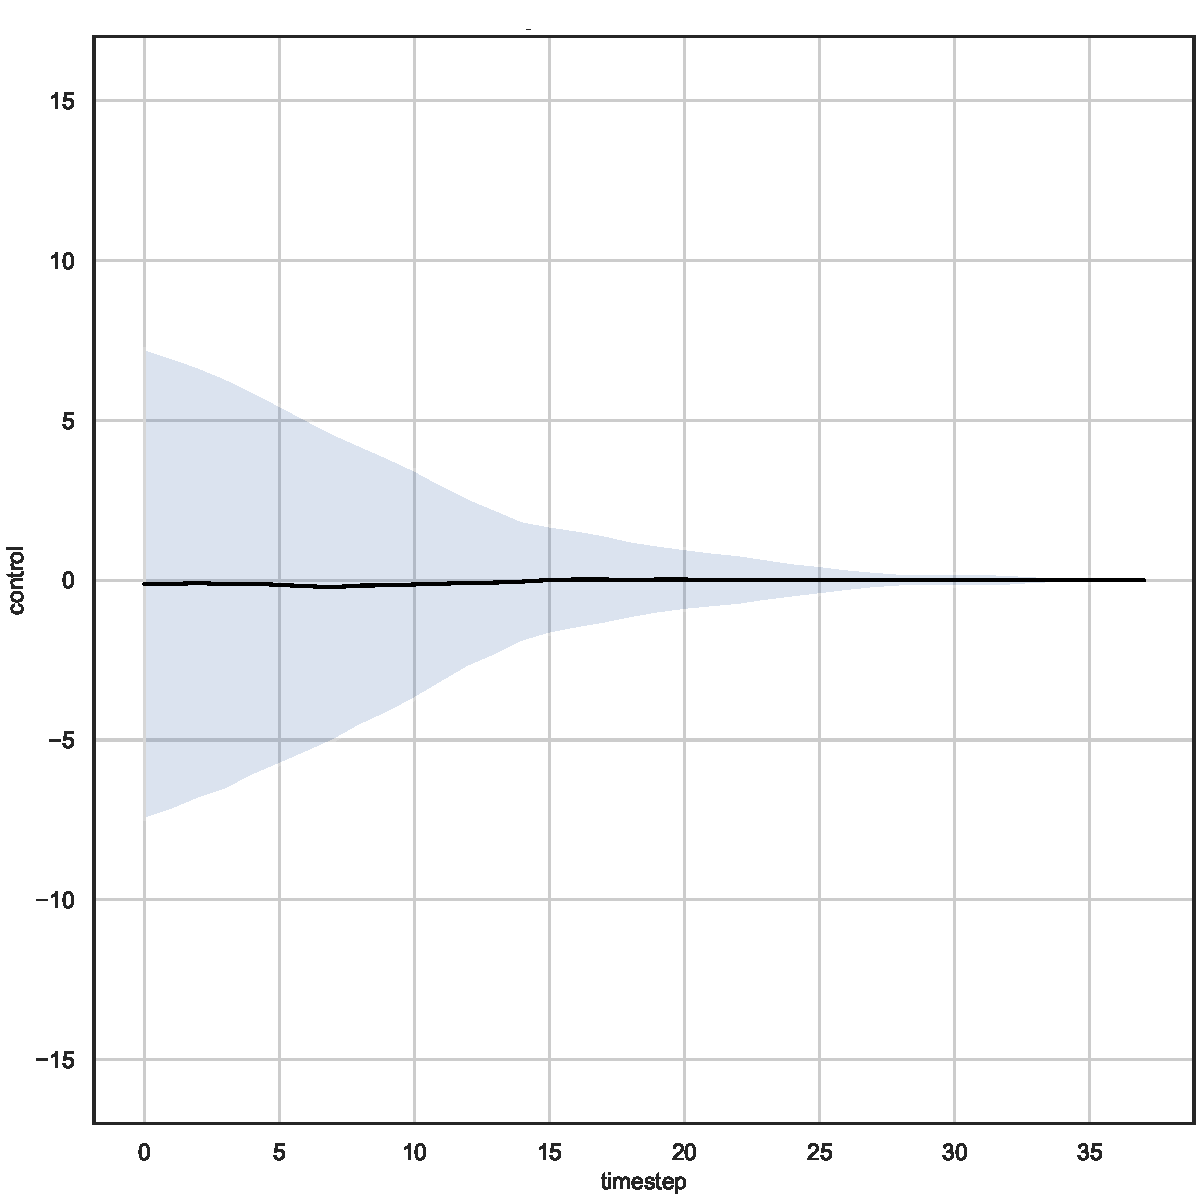
\includegraphics[width=\textwidth]{contents/images/net-d9/control-overtime-omniscient}%
			\caption{Expert control.}
		\end{subfigure}
		\hspace{1cm}
		\begin{subfigure}[h]{0.35\textwidth}
			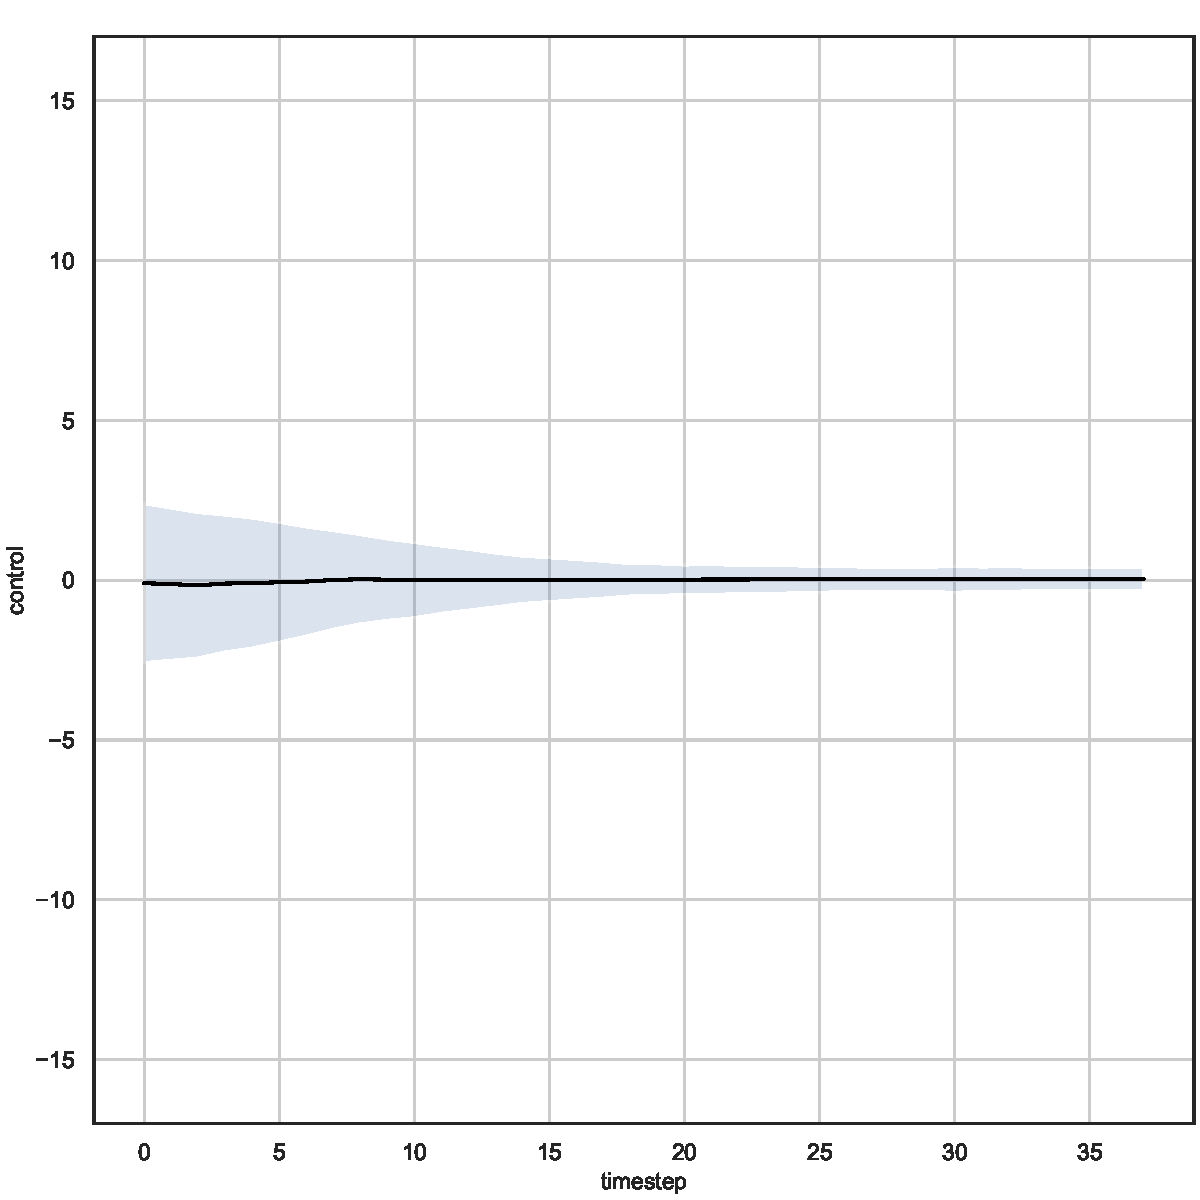
\includegraphics[width=\textwidth]{contents/images/net-d9/control-overtime-learned_distributed}
			\caption{Distributed control.}
		\end{subfigure}
	\end{center}
	\begin{center}
		\begin{subfigure}[h]{0.35\textwidth}			
			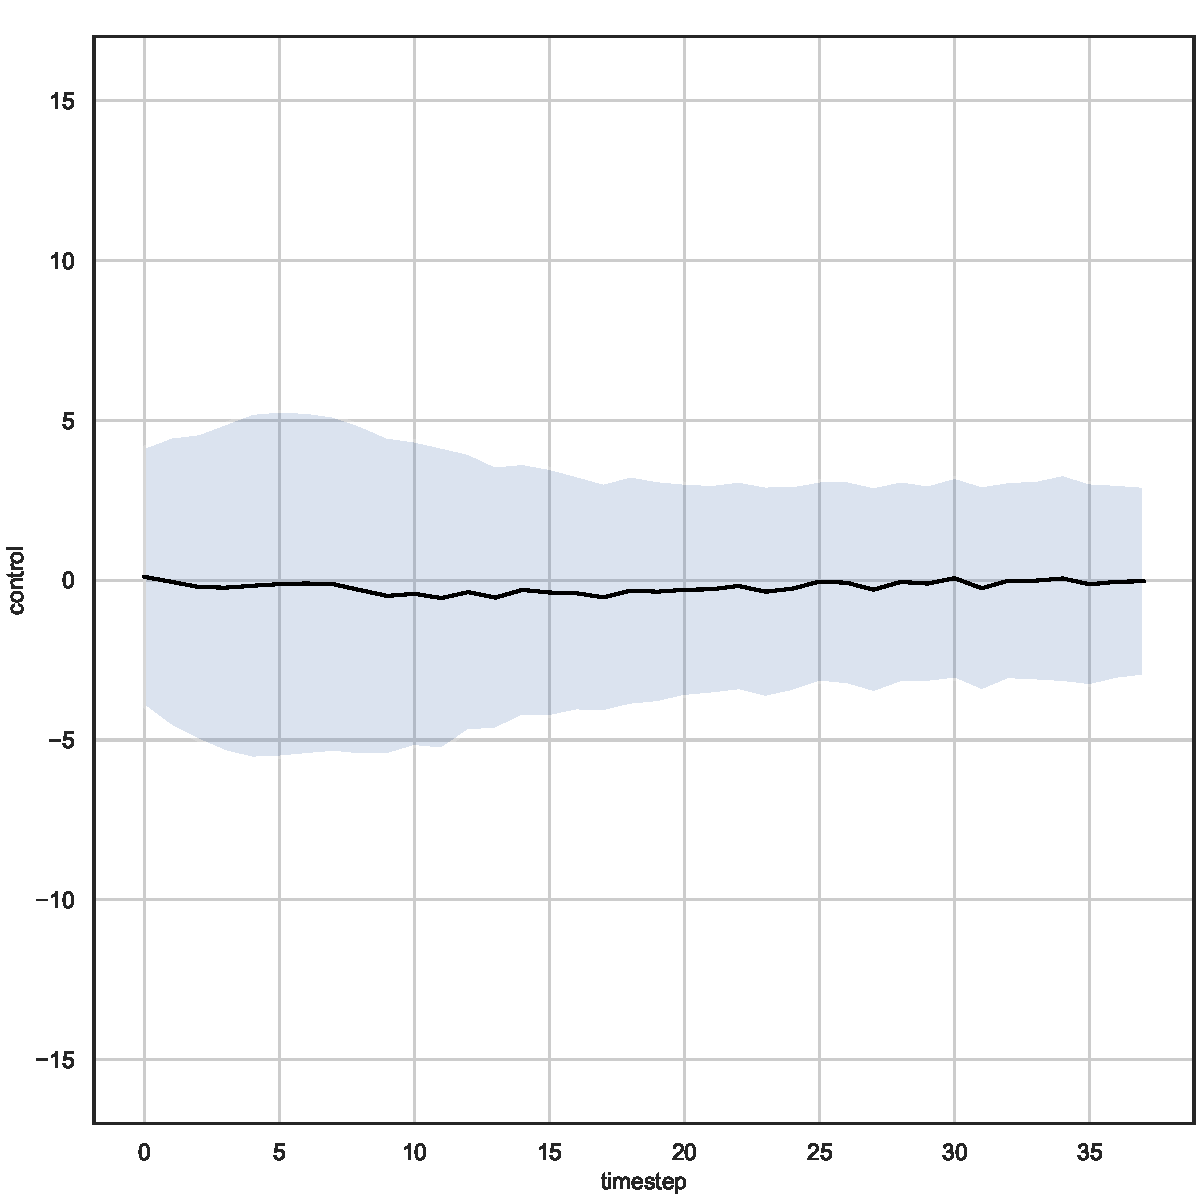
\includegraphics[width=\textwidth]{contents/images/net-d9/control-overtime-manual}%
			\caption{Manual control.}
		\end{subfigure}
		\hspace{1cm}
		\begin{subfigure}[h]{0.35\textwidth}
			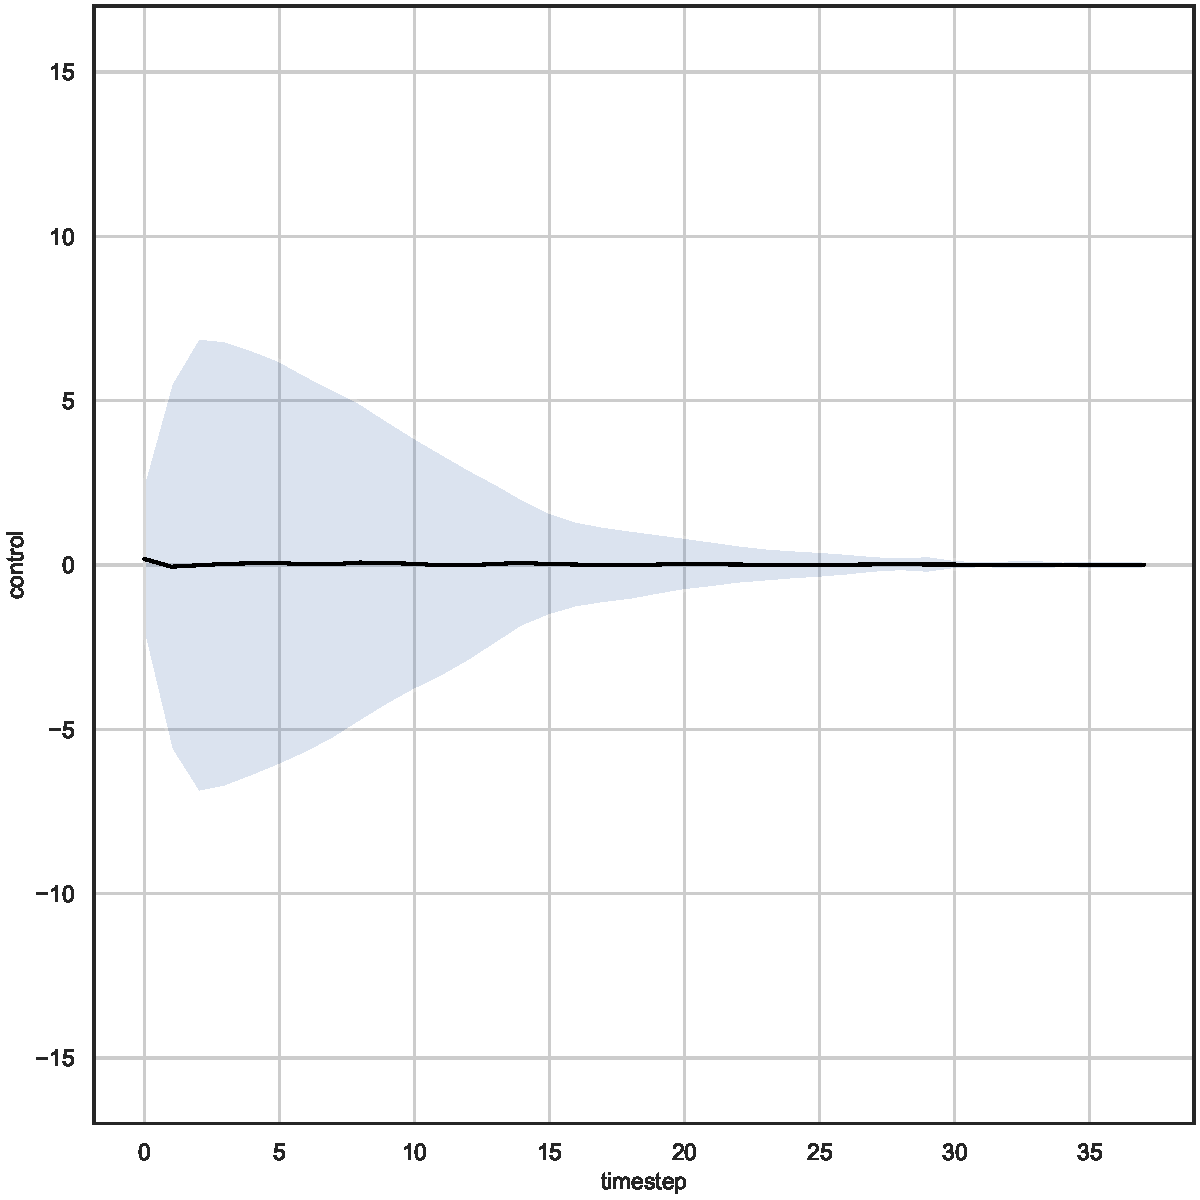
\includegraphics[width=\textwidth]{contents/images/net-c9/control-overtime-learned_communication}
			\caption{Communication control.}
		\end{subfigure}
	\end{center}
	\vspace{-0.5cm}
	\caption[Evaluation of the control decided by \texttt{net-c9}.]{Comparison of 
	output control decided using four controllers: the expert, the manual and the 
	two learned from \texttt{net-d9} and \texttt{net-c9}.}
	\label{fig:net-c9control}
\end{figure}

In Figure \ref{fig:net-c9responseposition} is displayed the behaviour of a robot 
located between two stationary agents which are already in the correct position, 
showing the response of the controllers, on the y-axis, by varying the position of 
the moving robot, visualised on the x-axis. As expected, the output is a high 
value, positive or negative respectively when the robot is close to an obstacle on 
the left or on the right, or it is close to $0$ when the distance from right and left 
is equal.
\begin{figure}[!htb]
	\centering
	\includegraphics[width=.45\textwidth]{contents/images/net-c9/response-varying_init_position-communication}%
	\caption{Response of \texttt{net-c9} by varying the initial position.}
	\label{fig:net-c9responseposition}
\end{figure}

Finally, in terms of absolute distance of each robot from the target, in Figure 
\ref{fig:net-c9distance} we show that exploiting the communication, the robots 
are able to end up in the correct position by using a couple more time steps than 
expert does. 
\begin{figure}[!htb]
	\centering
	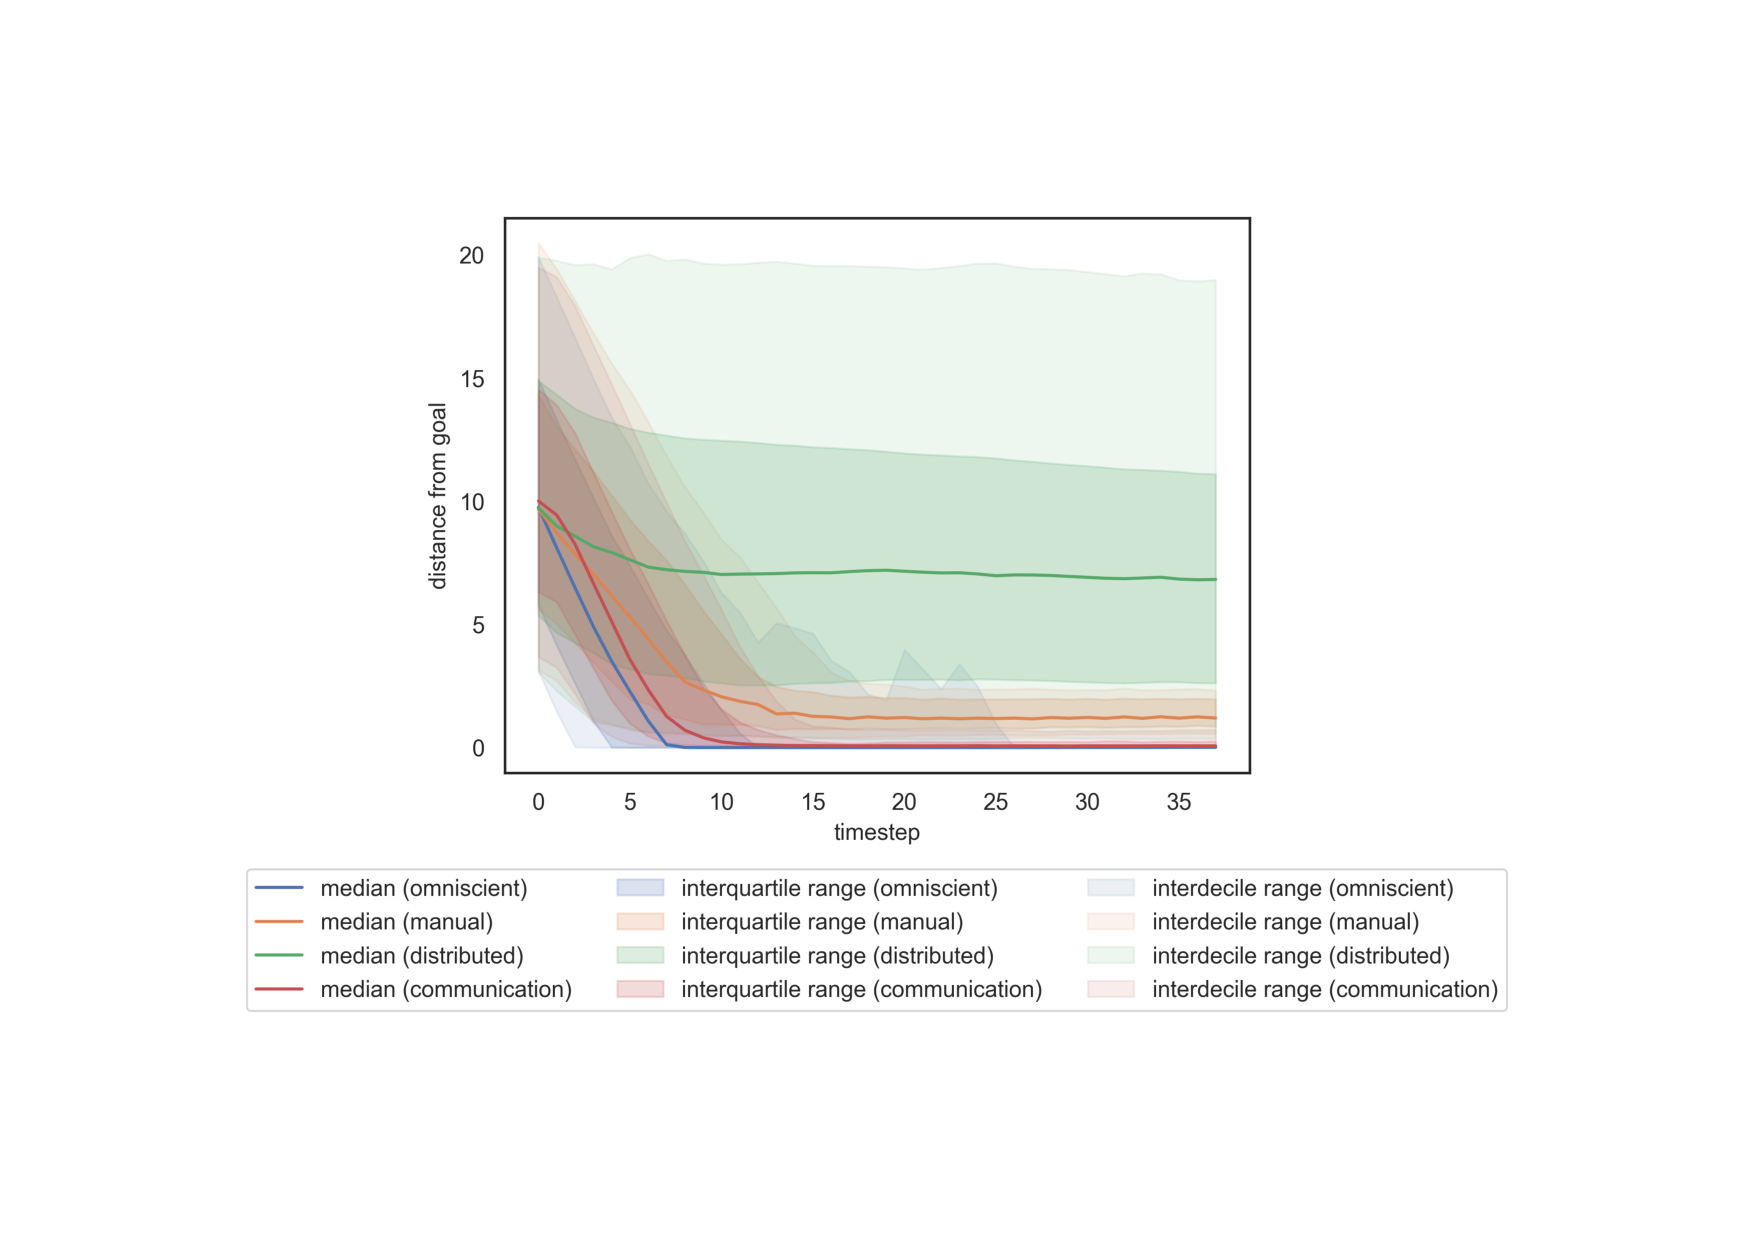
\includegraphics[width=.65\textwidth]{contents/images/net-c9/distances-from-goal-compressed-communication}%
	\caption[Evaluation of \texttt{net-c9} distances from goal.]{Comparison of 
		performance in terms of distances from goal obtained using four controllers: 
		the expert, the manual and the two learned from \texttt{net-d9} and 
		\texttt{net-c9}.}
	\label{fig:net-c9distance}
\end{figure}

In this case, the analysis of the communication transmitted over time, in Figure 
\ref{fig:net-c9comm}, denies the assumptions made previously. The robots do not 
decrease or increase the value transmitted by approaching the target, 
demonstrating, as anticipated the that this value is uncorrelated to the distance 
from goal, reaffirming the difficulty of understanding the protocol learned from 
the network.
\begin{figure}[!htb]
	\centering
	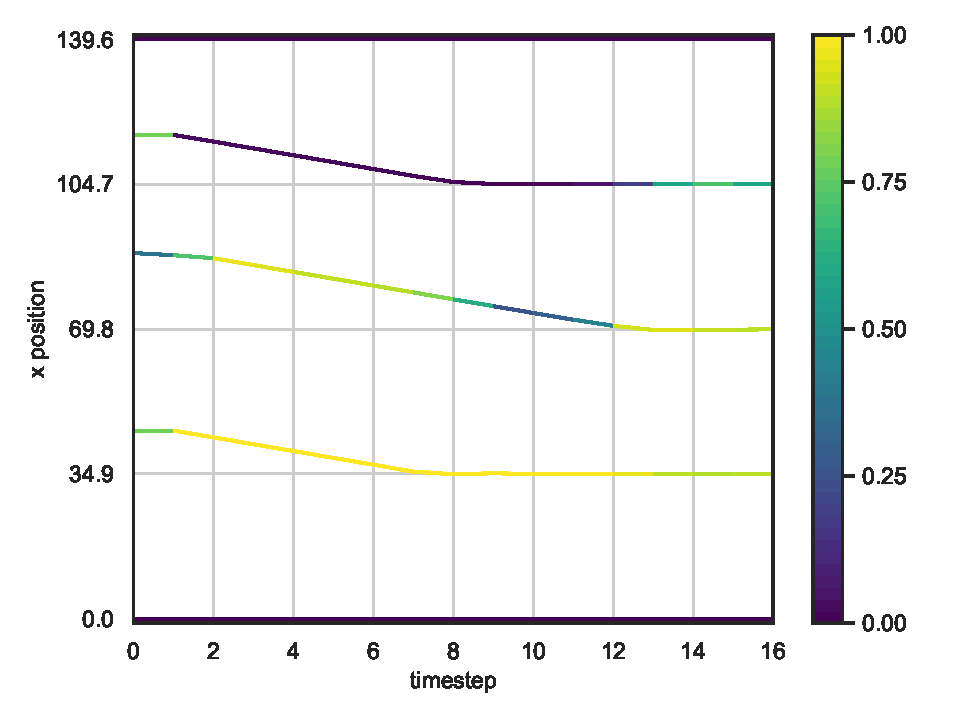
\includegraphics[width=.65\textwidth]{contents/images/net-c9/1/plot-simulation-communication-1}
	\vspace{-0.5cm}
	\caption[Evaluation of the communication learned by 
	\texttt{net-c9}.]{Visualisation of the communication values transmitted by each 
		robot over time using the controller learned from \texttt{net-c9}.}	
	\label{fig:net-c9comm}
\end{figure}

To sum up, we show once again in the figures below the losses of the trained 
models as the different inputs vary for each gap. In all the figures the blue line 
represents the loss using \texttt{prox\_values} as input, in orange 
\texttt{prox\_comm} and finally in green \texttt{all\_sensors}.
In case of an \texttt{avg\_gap} of $8$\gls{cm}, with or without communication, 
the model trained using \texttt{prox\_values} has a lower loss, followed, with a 
very close value, by the network that employ \texttt{all\_sensors}.
Next is the model that works with \texttt{prox\_comm}, that is not able to work 
well with small gaps. Even using the communication the performance become 
even worse than before. 
Similarly, by increasing the gap to $13$\gls{cm}, \texttt{prox\_values} alone is not 
able to achieve satisfactory results in both approaches, while used together with 
\texttt{prox\_comm}, \texttt{all\_sensors} reaches good performances, which can 
even be improved by using communication.
Finally, by increasing the gap even more, up to $24$\gls{cm}, 
\texttt{prox\_values} becomes completely unusable, while \texttt{prox\_comm} 
and \texttt{all\_sensors} have excellent responses, in particular with the new 
approach.
\begin{figure}[!htb]
	\begin{center}
		\begin{subfigure}[h]{0.32\textwidth}
		\includegraphics[width=\textwidth]{contents/images/task1-comm/loss-distributed-gap_8@copy}
		\caption{\texttt{avg\_gap} of $8$\gls{cm}.}
		\end{subfigure}
		\hfill
		\begin{subfigure}[h]{0.32\textwidth}
			\includegraphics[width=\textwidth]{contents/images/task1-comm/loss-distributed-gap_13@copy}%
			\caption{\texttt{avg\_gap} of $13$\gls{cm}.}
		\end{subfigure}
		\hfill
		\begin{subfigure}[h]{0.32\textwidth}
			\includegraphics[width=\textwidth]{contents/images/task1-comm/loss-distributed-gap_24@copy}
			\caption{\texttt{avg\_gap} of $24$\gls{cm}.}
		\end{subfigure}
	\end{center}
	\vspace{-0.5cm}
	\caption[Losses summary of the first set of experiments (no 
	communication).]{Comparison of the losses of the model trained without 
		communication, by varying the input of the networks for the three gaps.}
	\label{fig:distlossgaps}
\end{figure}

\begin{figure}[!htb]
	\begin{center}
		\begin{subfigure}[h]{0.32\textwidth}
			\includegraphics[width=\textwidth]{contents/images/task1-comm/loss-communication-gap_8@copy}%
			\caption{\texttt{avg\_gap} of $8$\gls{cm}.}
		\end{subfigure}
		\hfill
		\begin{subfigure}[h]{0.32\textwidth}
			\includegraphics[width=\textwidth]{contents/images/task1-comm/loss-communication-gap_13@copy}%
			\caption{\texttt{avg\_gap} of $13$\gls{cm}.}
		\end{subfigure}
		\hfill
		\begin{subfigure}[h]{0.32\textwidth}
			\includegraphics[width=\textwidth]{contents/images/task1-comm/loss-communication-gap_24@copy}
			\caption{\texttt{avg\_gap} of $24$\gls{cm}.}
		\end{subfigure}
	\end{center}
	\vspace{-0.5cm}
	\caption[Losses summary of the first set of experiments 
	(communication).]{Comparison of the losses of the model trained with 
		communication, by varying the input of the networks for the three gaps.}
	\label{fig:commloss81324}
\end{figure}

The last group of experiments we carried out using a distributed approach with 
communication, summarised in Table \ref{tab:modelcomm}, examines the 
behaviour of the control learned using \texttt{all\_sensors} inputs. 
\begin{figure}[!htb]
	\centering
	\begin{tabular}{ccccc}
		\toprule
		\textbf{Model} \quad & \textbf{\texttt{network\_input}} & 
		\textbf{\texttt{input\_size}} & \textbf{\texttt{avg\_gap}} & \textbf{\texttt{N}}\\
		\midrule
		\texttt{net-c10} 	& \texttt{all\_sensors}		&  $14$  &  $8$		 	 &	 $5$ \\
		\texttt{net-c11} 	& \texttt{all\_sensors}		&  $14$  &  $20$		&	$5$ \\
		\texttt{net-c12} 	& \texttt{all\_sensors}		&  $14$  &  variable   &    $5$\\
		\texttt{net-c13} 	& \texttt{all\_sensors}	  	&  $14$  &  $8$			 &	  $8$ \\
		\texttt{net-c14} 	& \texttt{all\_sensors}	  	&  $14$  &  $20$   		&	 $8$ \\
		\texttt{net-c15} 	& \texttt{all\_sensors}	  	&  $14$  &  variable	&	 $8$ \\
		\texttt{net-c16} 	& \texttt{all\_sensors}	  	&  $14$  &  $ 8$		  &	 variable\\
		\texttt{net-c17} 	& \texttt{all\_sensors}	  	&  $14$  &  $20$		 &	variable\\
		\texttt{net-c18} 	& \texttt{all\_sensors}	  	&  $14$  &  variable	 &	
		variable\\
		\bottomrule
	\end{tabular}
	\captionof{table}[Experiments with variable agents and gaps 
	(communication).]{List of the experiments carried out using a variable number 
		of agents and of gap.}
	\label{tab:modelcomm}
\end{figure}

The objective of this set of experiments is verify the robustness of the models, 
proving that it is possible to train networks that use a variable number of agents.
We analyse the same experiments of the previous approach.
We focus our examination by inspecting the behaviour of the network trained on 
simulations with different number of robots $N$ and variable average gap, i.e 
\texttt{net-c12}, \texttt{net-c15} and \texttt{net-c18}. Then we compare 
the 
performances obtained for these models to the corresponding distributed 
networks, i.e \texttt{net-d12}, \texttt{net-d15} and \texttt{net-d18}.

First of all we start by showing in Figure \ref{fig:commexlossallt} an overview of 
the train and validation losses obtained for these models.
\begin{figure}[!htb]
	\centering
	\includegraphics[width=.8\textwidth]{contents/images/task1-comm-extension/loss-communication-all@}%
	\caption[Comparison of losses of the second set of experiments.]{Comparison 
		of the losses of the models carried out using a variable number of agents and 
		of average gap.}
	\label{fig:commexlossallt}
\end{figure}

Proceeding step by step we summarise in Figure \ref{fig:commlossn5} the losses 
of the experiments carried out using a $5$ agents, the same of the first group of 
experiments presented above, in order to highlight the difference of performance 
using a gap that is first small, then large and finally variable, respectively 
represented by the blue, the orange and the green lines.
These results are also compared to those obtained without employing the 
communication.
Clearly, in case of small gaps the network performs better. We can also note that 
in general by enable the communication the losses decrease, meaning an 
improvement over the previous approach.
\begin{figure}[!htb]
	\begin{center}
		\begin{subfigure}[h]{0.49\textwidth}
			\centering
			\includegraphics[width=.7\textwidth]{contents/images/task1-comm-extension/loss-distributed-N5@copy}
			\caption{Distributed approach.}
		\end{subfigure}
		\hfill
		\begin{subfigure}[h]{0.49\textwidth}
			\centering
			\includegraphics[width=.7\textwidth]{contents/images/task1-comm-extension/loss-communication-N5@copy}
			\caption{Distributed approach with communication.}
		\end{subfigure}	
	\end{center}
	\vspace{-0.5cm}
	\caption{Comparison of the losses of the models that use $5$ agents as the gap 
		varies.}
	\label{fig:commlossn5}
\end{figure}

Considering as foretold the model trained using an average gap, in Figure 
\ref{fig:net-c12r2} are shown the \gls{r2} coefficients of the manual and the 
learned controllers, in both cases, i.e. with and without communication, on the 
validation sets.
From these figures we expect that the behaviour of the robots using the 
learned controller with communication instead of the manual or the 
distributed alone is better, even if far from the expert. The new model produces 
an increase in the coefficient \gls{r2} from $0.41$ to $0.49$.
\begin{figure}[!htb]
	\begin{center}
		\begin{subfigure}[h]{0.49\textwidth}
			\includegraphics[width=\textwidth]{contents/images/net-d12/regression-net-d12-vs-omniscient}%
		\end{subfigure}
		\hfill\vspace{-0.5cm}
		\begin{subfigure}[h]{0.49\textwidth}
			\includegraphics[width=\textwidth]{contents/images/net-c12/regression-net-c12-vs-omniscient}%
		\end{subfigure}
	\end{center}
	\caption[Evaluation of the \gls{r2} coefficients of \texttt{net-c12}.]{Comparison 
		of the \gls{r2} coefficients of the controllers learned from 
		\texttt{net-d12} and \texttt{net-c12}, with respect to the omniscient one.}
	\label{fig:net-c12r2}
\end{figure}

\begin{figure}[!htb]
	\begin{center}
		\begin{subfigure}[h]{0.49\textwidth}
			\centering
			\includegraphics[width=.9\textwidth]{contents/images/net-d12/position-overtime-omniscient}%
			\caption{Expert controller trajectories.}
		\end{subfigure}
		\hfill
		\begin{subfigure}[h]{0.49\textwidth}
			\centering
			\includegraphics[width=.9\textwidth]{contents/images/net-d12/position-overtime-learned_distributed}
			\caption{Distributed controller trajectories.}
		\end{subfigure}
	\end{center}
	\begin{center}
		\begin{subfigure}[h]{0.49\textwidth}
			\centering			
			\includegraphics[width=.9\textwidth]{contents/images/net-d12/position-overtime-manual}%
			\caption{Manual controller trajectories.}
		\end{subfigure}
		\hfill
		\begin{subfigure}[h]{0.49\textwidth}
			\centering
			\includegraphics[width=.9\textwidth]{contents/images/net-c12/position-overtime-learned_communication}
			\caption{Communication controller trajectories.}
		\end{subfigure}
	\end{center}
	\vspace{-0.5cm}
	\caption[Evaluation of the trajectories learned by \texttt{net-c12}.]{Comparison 
	of trajectories generated using four controllers: the expert, the manual and 
	the two learned from \texttt{net-d12} and \texttt{net-c12}.}
	\label{fig:net-c12traj}
\end{figure}
Analysing in Figure \ref{fig:net-c12traj} the trajectories obtained employing the 
four controllers it is difficult to demonstrate the improvement over the previous 
approach as having a variable gap we observe a deviation of the position of the 
robots with respect to the average that in this case it does not indicate a limitation 
of the model but just that the target positions are different among the simulation 
runs. 

An analysis of the evolution of the control over time in Figure 
\ref{fig:net-c12control} evidence that the control decided by the communication 
network is similar to that set by the expert.
\begin{figure}[!htb]
	\begin{center}
		\begin{subfigure}[h]{0.35\textwidth}
			\includegraphics[width=\textwidth]{contents/images/net-d12/control-overtime-omniscient}%
			\caption{Expert control.}
		\end{subfigure}
		\hspace{1cm}
		\begin{subfigure}[h]{0.35\textwidth}
			\includegraphics[width=\textwidth]{contents/images/net-d12/control-overtime-learned_distributed}
			\caption{Distributed control.}
		\end{subfigure}
	\end{center}
	\begin{center}
		\begin{subfigure}[h]{0.35\textwidth}			
			\includegraphics[width=\textwidth]{contents/images/net-d12/control-overtime-manual}%
			\caption{Manual control.}
		\end{subfigure}
		\hspace{1cm}
		\begin{subfigure}[h]{0.35\textwidth}
			\includegraphics[width=\textwidth]{contents/images/net-c12/control-overtime-learned_communication}
			\caption{Communication control.}
		\end{subfigure}
	\end{center}
	\vspace{-0.5cm}
	\caption[Evaluation of the control decided by \texttt{net-c12}.]{Comparison of 
	output control decided using four controllers: the expert, the manual and the 
	two learned from \texttt{net-d12} and \texttt{net-c12}.}
	\label{fig:net-c12control}
\end{figure}

In Figure \ref{fig:net-c12responseposition} is displayed the behaviour of a robot 
located between two stationary agents which are already in the correct position, 
showing the response of the controllers, on the y-axis, by varying the position of 
the moving robot, on the x-axis.  
As expected, the output is a high positive value when the robot is close to an 
obstacle on the left, negative when there is an obstacle in front and not behind, 
and $0$ when the distance from right and left is equal.
The behaviour of the controller that uses the communication is the most accurate 
when the moving robot is halfway between the two stationary.
\begin{figure}[!htb]
	\centering
	\includegraphics[width=.45\textwidth]{contents/images/net-c12/response-varying_init_position-communication}%
	\caption{Response of \texttt{net-c12} by varying the initial position.}
	\label{fig:net-c12responseposition}
\end{figure}

Finally, in Figure \ref{fig:net-c12distance} are presented the absolute distances of 
each robot from the target, visualised on the y-axis, over time.
On average, the distance from goal of the communication controller is a bit better 
than that obtained with the distributed while similar to the manual, even if slower. 
In the final configuration in all three cases the agents are $1$\gls{cm} away from 
the target. 
\begin{figure}[H]
	\centering
	\includegraphics[width=.65\textwidth]{contents/images/net-c12/distances-from-goal-compressed-communication}%
	\caption[Evaluation of \texttt{net-c12} distances from goal.]{Comparison of 
		performance in terms of distances from goal obtained using four controllers: 
		the expert, the manual and the two learned from \texttt{net-d12} and 
		\texttt{net-c12}.}
	\label{fig:net-c12distance}
\end{figure}

Following are presented the results of the experiments performed using 
$8$ agents. In Figure \ref{fig:commlossN8}, are shown the losses by varying the 
average gap, as before the blue, orange and green lines represent respectively 
gaps of $8$\gls{cm}, $20$\gls{cm} and variable. From a first observation we see 
that the network perform better in case of small gaps and moreover the approach 
with communication demonstrate lower loss values than the previous one.
\begin{figure}[!htb]
	\begin{center}
		\begin{subfigure}[h]{0.49\textwidth}
			\centering
			\includegraphics[width=.7\textwidth]{contents/images/task1-comm-extension/loss-distributed-N8@copy}
			\caption{Distributed approach.}
		\end{subfigure}
		\hfill
		\begin{subfigure}[h]{0.49\textwidth}
			\centering
			\includegraphics[width=.7\textwidth]{contents/images/task1-comm-extension/loss-communication-N8@copy}
			\caption{Distributed approach with communication.}
		\end{subfigure}	
	\end{center}
	\vspace{-0.5cm}
	\caption{Comparison of the losses of the models that use $8$ agents as the gap 
		varies.}
	\label{fig:commlossN8}
\end{figure}

Focusing on the models that use the dataset generate using a variable average 
gap, in Figure \ref{fig:net-c15r2} we observe the \gls{r2} of the manual and the 
learned controllers, both the one with and the one without communication, on 
the validation sets.
Given the fact that the coefficient is increased from $0.23$ up to $0.32$ we 
expect superior performance.  
\begin{figure}[!htb]
	\begin{center}
		\begin{subfigure}[h]{0.49\textwidth}
			\includegraphics[width=\textwidth]{contents/images/net-d15/regression-net-d15-vs-omniscient}%
		\end{subfigure}
		\hfill\vspace{-0.5cm}
		\begin{subfigure}[h]{0.49\textwidth}
			\includegraphics[width=\textwidth]{contents/images/net-c15/regression-net-c15-vs-omniscient}%
		\end{subfigure}
	\end{center}
	\caption[Evaluation of the \gls{r2} coefficients of \texttt{net-c15}.]{Comparison 
		of the \gls{r2} coefficients of the controllers learned from 
		\texttt{net-d15} and \texttt{net-c15}, with respect to the omniscient one.}
	\label{fig:net-c15r2}
\end{figure}

In Figure \ref{fig:net-c15traj} are shown the trajectories obtained employing the 
four controllers.  On average, all the robots seems to approach the desired 
position, some with less and some with more time steps, but as before it is difficult 
to demonstrate improvement over the previous approach due to the deviation in 
the graph caused by the different target positions.

Even the analysis of the evolution of the control over time in Figure 
\ref{fig:net-c15control} is not able to provide further considerations.
\begin{figure}[!htb]
	\begin{center}
		\begin{subfigure}[h]{0.49\textwidth}
			\centering
			\includegraphics[width=.9\textwidth]{contents/images/net-d15/position-overtime-omniscient}%
			\caption{Expert controller trajectories.}
		\end{subfigure}
		\hfill
		\begin{subfigure}[h]{0.49\textwidth}
			\centering
			\includegraphics[width=.9\textwidth]{contents/images/net-d15/position-overtime-learned_distributed}
			\caption{Distributed controller trajectories.}
		\end{subfigure}
	\end{center}
	\vspace{-0.5cm}
	\caption[Evaluation of the trajectories learned by \texttt{net-c15}.]{Comparison 
		of trajectories generated using four controllers: the expert, the manual and 
		the two learned from \texttt{net-d15} and \texttt{net-c15}.}	
\end{figure}

\medskip
\begin{figure}[!htb]\ContinuedFloat
	\begin{center}
		\begin{subfigure}[h]{0.49\textwidth}
			\centering			
			\includegraphics[width=.9\textwidth]{contents/images/net-d15/position-overtime-manual}%
			\caption{Manual controller trajectories.}
		\end{subfigure}
		\hfill
		\begin{subfigure}[h]{0.49\textwidth}
			\centering
			\includegraphics[width=.9\textwidth]{contents/images/net-c15/position-overtime-learned_communication}
			\caption{Communication controller trajectories.}
		\end{subfigure}
	\end{center}
	\vspace{-0.5cm}
	\caption[]{Comparison of trajectories generated using four controllers: the 
		expert, the manual and the two learned from \texttt{net-d15} and 
		\texttt{net-c15} (cont.).}
	\label{fig:net-c15traj}
\end{figure}
\begin{figure}[H]
	\begin{center}
		\begin{subfigure}[h]{0.35\textwidth}
			\includegraphics[width=\textwidth]{contents/images/net-d15/control-overtime-omniscient}%
			\caption{Expert control.}
		\end{subfigure}
		\hspace{1cm}
		\begin{subfigure}[h]{0.35\textwidth}
			\includegraphics[width=\textwidth]{contents/images/net-d15/control-overtime-learned_distributed}
			\caption{Distributed control.}
		\end{subfigure}
	\end{center}
	\begin{center}
		\begin{subfigure}[h]{0.35\textwidth}			
			\includegraphics[width=\textwidth]{contents/images/net-d15/control-overtime-manual}%
			\caption{Manual control.}
		\end{subfigure}
		\hspace{1cm}
		\begin{subfigure}[h]{0.35\textwidth}
			\includegraphics[width=\textwidth]{contents/images/net-c15/control-overtime-learned_communication}
			\caption{Communication control.}
		\end{subfigure}
	\end{center}
	\vspace{-0.5cm}
	\caption[Evaluation of the control decided by \texttt{net-c15}.]{Comparison of 
	output control decided using four controllers: the expert, the manual and the 
	two learned from \texttt{net-d15} and \texttt{net-c15}.}
	\label{fig:net-c15control}
\end{figure}

In Figure \ref{fig:net-c15responseposition} is displayed the behaviour of a robot 
located between two stationary agents, showing the response of the controllers, 
on the y-axis, by varying the position of the moving robot, visualised on the 
x-axis.  
\begin{figure}[!htb]
	\centering
	\includegraphics[width=.45\textwidth]{contents/images/net-c15/response-varying_init_position-communication}%
	\caption{Response of \texttt{net-c15} by varying the initial position.}
	\label{fig:net-c15responseposition}
\end{figure}
This time the trend of the curve obtained from the communication controller is 
different than the desired one.

Finally, in Figure \ref{fig:net-c15distance} is presented a metric that measures the 
absolute distance of each robot from the target over time.
Unlike the non-optimal performance obtained with the distributed controller, in 
which the robots in the final configuration are located on average at about 
$5$\gls{cm} from the target, the distance from goal of the communication 
controller is far better but similar to that obtained with the manual. Even if the 
new approach need more time to converge, at the end the robots are $2$ away 
from the goal.
\begin{figure}[H]
	\centering
	\includegraphics[width=.65\textwidth]{contents/images/net-c15/distances-from-goal-compressed-communication}%
	\caption[Evaluation of \texttt{net-c15} distances from goal.]{Comparison of 
		performance in terms of distances from goal obtained using four controllers: 
		the expert, the manual and the two learned from \texttt{net-d15} and 
		\texttt{net-c15}.}
	\label{fig:net-c15distance}
\end{figure}

We conclude the experiment on task 1 presenting the results obtained using 
variable number of agents, in particular, in Figure \ref{fig:commlossNvar} are 
summarised the performance in terms of loss, as before we used blue, orange and 
green lines to represent respectively average gaps of $8$\gls{cm}, $13$\gls{cm} 
and variable.
Using the new approach we observe from the trend of the curves that in general 
the losses are decreased and for the network it is easier to perform the task by 
using a smaller gap.
\begin{figure}[!htb]
	\begin{center}
		\begin{subfigure}[h]{0.49\textwidth}
			\centering
			\includegraphics[width=.7\textwidth]{contents/images/task1-comm-extension/loss-distributed-Nvar@copy}
			\caption{Distributed approach.}
		\end{subfigure}
		\hfill
		\begin{subfigure}[h]{0.49\textwidth}
			\centering
			\includegraphics[width=.7\textwidth]{contents/images/task1-comm-extension/loss-communication-Nvar@copy}
			\caption{Distributed approach with communication.}
		\end{subfigure}	
	\end{center}
	\vspace{-0.5cm}
	\caption{Comparison of the losses of the models that use variable agents and 	
		gaps.}
	\label{fig:commlossNvar}
\end{figure}

Considering as before the more complex case, for instance the one with variable 
average gap, in Figure \ref{fig:net-c18r2} are visualised the \gls{r2} of 
the manual and the learned controllers, with and without communication.
A small improvement in the new approach is confirmed by the increase in the 
coefficient \gls{r2} from $0.23$ to $0.30$. 
\begin{figure}[!htb]
	\begin{center}
		\begin{subfigure}[h]{0.49\textwidth}
			\includegraphics[width=\textwidth]{contents/images/net-d18/regression-net-d18-vs-omniscient}%
		\end{subfigure}
		\hfill\vspace{-0.5cm}
		\begin{subfigure}[h]{0.49\textwidth}
			\includegraphics[width=\textwidth]{contents/images/net-c18/regression-net-c18-vs-omniscient}%
		\end{subfigure}
	\end{center}
	\caption[Evaluation of the \gls{r2} coefficients of 
	\texttt{net-c18}.]{Comparison 
		of the \gls{r2} coefficients of the manual and the controllers learned from 
		\texttt{net-d18} and \texttt{net-c18}, with respect to the omniscient 
		one.}
	\label{fig:net-c18r2}
\end{figure}

In this experiment is difficult to demonstrate improvement over the previous 
approach through the trajectories plots, as well as by the evolution of the control, 
due to the variable average gap. 

For this reason we move on analysing in Figure 
\ref{fig:net-c18responseposition} 
the behaviour of a robot located between two stationary agents which are already 
in the correct position, showing the response of the controllers by varying the 
position of the moving robot. 
\begin{figure}[!htb]
	\centering
	\includegraphics[width=.45\textwidth]{contents/images/net-c18/response-varying_init_position-communication}%
	\caption{Response of \texttt{net-c18} by varying the initial position.}
	\label{fig:net-c18responseposition}
\end{figure}

\noindent
As expected, the output is a high value, positive or 
negative respectively when the robot is close to an obstacle on the left or on 
the 
right, or it is close to $0$ when the distance from right and left is equal.

Finally, in terms of absolute distance of each robot from the target, in Figure 
\ref{fig:net-c18distance} we show that exploiting the communication, the 
robots 
in the final configuration are closer to the target than those moved using the 
distributed or even the manual controller.
\begin{figure}[!htb]
	\centering
	\includegraphics[width=.65\textwidth]{contents/images/net-c18/distances-from-goal-compressed-communication}%
	\caption[Evaluation of \texttt{net-c18} distances from goal.]{Comparison 
	of 
		performance in terms of distances from goal obtained using four controllers: 
		the expert, the manual and the two learned from \texttt{net-d18} and 
		\texttt{net-c18}.}
	\label{fig:net-c18distance}
\end{figure}

To sum up, we finally show in the figures below the losses of the trained 
models as the number of agents vary for each gap. In all the figures are 
represented the losses of the models that use $5$, $8$ and variable agents, 
respectively in blue, orange and green.
In case of an \texttt{avg\_gap} of $8$\gls{cm}, with or without communication, 
the model trained using a minor number of agents, as expected, has a lower loss.
Instead, very similar are the losses obtained in case of $8$ or variable agents, in 
which the model with less robots is still the better.
In general, using the communication has improved the performance.

\begin{figure}[!htb]
	\begin{center}
		\begin{subfigure}[h]{0.32\textwidth}
			\includegraphics[width=\textwidth]{contents/images/task1-comm-extension/loss-distributed-gap_8@copy}
			\caption{\texttt{avg\_gap} of $8$\gls{cm}.}
		\end{subfigure}
		\hfill
		\begin{subfigure}[h]{0.32\textwidth}
			\includegraphics[width=\textwidth]{contents/images/task1-comm-extension/loss-distributed-gap_20@copy}%
			\caption{\texttt{avg\_gap} of $13$\gls{cm}.}
		\end{subfigure}
		\hfill
		\begin{subfigure}[h]{0.32\textwidth}
			\includegraphics[width=\textwidth]{contents/images/task1-comm-extension/loss-distributed-gap_var@copy}
			\caption{\texttt{avg\_gap} of $24$\gls{cm}.}
		\end{subfigure}
	\end{center}
	\vspace{-0.5cm}
	\caption[Losses summary of the second set of experiments (no 
	communication).]{Comparison of the losses of the model trained without 
		communication, by varying the number of agents for the three gaps.}
	\label{fig:distlossgapsexte}
\end{figure}
\begin{figure}[!htb]
	\begin{center}
		\begin{subfigure}[h]{0.32\textwidth}
			\includegraphics[width=\textwidth]{contents/images/task1-comm-extension/loss-communication-gap_8@copy}%
			\caption{\texttt{avg\_gap} of $8$\gls{cm}.}
		\end{subfigure}
		\hfill
		\begin{subfigure}[h]{0.32\textwidth}
			\includegraphics[width=\textwidth]{contents/images/task1-comm-extension/loss-communication-gap_20@copy}%
			\caption{\texttt{avg\_gap} of $13$\gls{cm}.}
		\end{subfigure}
		\hfill
		\begin{subfigure}[h]{0.32\textwidth}
			\includegraphics[width=\textwidth]{contents/images/task1-comm-extension/loss-communication-gap_var@copy}
			\caption{\texttt{avg\_gap} of $24$\gls{cm}.}
		\end{subfigure}
	\end{center}
	\vspace{-0.5cm}
	\caption[Losses summary of the second set of experiments 
	(communication).]{Comparison of the losses of the model trained with 
		communication, by varying the number of agents for the three gaps.}
	\label{fig:commlossexte81324}
\end{figure}


\subsubsection{Summary}
\label{subsubsec:commsummary}
In this section we have shown that using a distributed controller learned by 
imitating an expert and exploiting a communication protocol among the 
agents, it is possible to obtain results more or less comparable to those reached 
employing an expert controller, while a bit worse when using variable number of 
agents and gaps.
